\PassOptionsToPackage{american}{babel}
\documentclass[letterpaper,12pt,twoside,onecolumn,openright,final]{memoir}
\usepackage[american]{babel}
\usepackage[backend=biber,style=authortitle-ibid,sortcites=true,sorting=nyt]{biblatex}
\usepackage{booktabs}
\addbibresource{./MainstreamingPipeline.bib}
\usepackage{etex}
\usepackage{rotating}
\usepackage{float}
\usepackage{afterpage}
\usepackage{caption}
\usepackage{blindtext}
\usepackage{tabularx}
\usepackage{graphicx}
\graphicspath{ {images/}}
\renewcommand\cftappendixname{\appendixname~}
\usepackage{pdfpages}
\usepackage{csquotes}
\usepackage{setspace}
\usepackage{url}
\setcounter{tocdepth}{0}
\usepackage{xcolor}
\usepackage{bookman} 
\usepackage{endnotes}
\usepackage{longtable}
\usepackage{array}
\newlength\mylength
\usepackage{pdflscape}
\usepackage{geometry}
\DeclareCaptionFont{tiny}{\tiny}
\let\footnote=\endnote
%
\raggedbottom
\midsloppy
\nobibintoc
%
\AtBeginDocument{
	\addtolength{\cftchapternumwidth}{2.5em}
	\addtolength{\cftpartnumwidth}{2.5em}
}
\newenvironment{dedication}
{
	\cleardoublepage
	\thispagestyle{empty}
	\vspace*{\stretch{1}}
	\hfill\begin{minipage}[t]{1.0\textwidth}
		\raggedright
	}%
	{
	\end{minipage}
	\vspace*{\stretch{3}}
	\clearpage
}
%
\newenvironment{AboutAuthor}
{
	\cleardoublepage
	\thispagestyle{empty}
	\vspace*{\stretch{1}}
	\hfill\begin{minipage}[t]{1.0\textwidth}
		\raggedright
	}%
	{
	\end{minipage}
	\vspace*{\stretch{3}}
	\clearpage
}
%
%%%%%%%%%%%%%%%%%%%%%%%%%%%%%%%%%%%%%%%%%%%%
%
% End Preamble
%
%%%%%%%%%%%%%%%%%%%%%%%%%%%%%%%%%%%%%%%%%%%%
% 
%%%%%%%%%%%%%%%%%%%%%%%%%%%%%%%%%%%%%%%%%%%%
%
% Begin Front Matter
%
%%%%%%%%%%%%%%%%%%%%%%%%%%%%%%%%%%%%%%%%%%%%
%
\frontmatter
\makepagestyle{mystyle} 
\setlength{\headwidth}{\textwidth+\marginparsep+\marginparwidth\relax}
\makerunningwidth{mystyle}{\headwidth}
\makeevenhead{mystyle}{\itshape\leftmark}{}{} 
\makeoddhead{mystyle}{}{}{\itshape\leftmark} 
\makeevenfoot{mystyle}{\thepage}{}{} 
\makeoddfoot{mystyle}{}{}{\thepage} 
\makeatletter
\makepsmarks{mystyle}{%
	\createmark{chapter}{left}{shownumber}{\@chapapp\ }{.\ }}
\makeatother
%
\makepagestyle{plain}
\makerunningwidth{plain}{\headwidth}
\makeevenfoot{plain}{\thepage}{}{}
\makeoddfoot{plain}{}{}{\thepage}
%
\hbox{
	\hspace*{0.2\textwidth}
	\rule{2.5pt}{\textheight-5pt*1\relax}
	\hspace*{0.05\textwidth}
	\parbox[b]{0.75\textwidth}{
		\vbox{
			{\noindent\huge\bfseries Why Haven't They}\\
			{\noindent\huge\bfseries Done That Yet?}\\[1\baselineskip]
			{\Large\itshape Methods to Successfully Include Autistic Students in the General Education Classroom}\\[3\baselineskip]}
		{\Large Michael Ryan Hunsaker, Ph.D.}\par
		\vspace{0.5\textheight}
		{\noindent \begin{copyright}~~~The Author\end{copyright}}
		\\
		\\
	}
}
%
\begin{document}
%
\cleardoublepage
%
\begin{dedication}
	For Kyle
\end{dedication}
%
\begin{KeepFromToc}
	\tableofcontents*
\end{KeepFromToc}
%
\clearpage
\listoffigures
\listoftables
\cleardoublepage
%
\chapter[Prologue]{Prologue}
From 1999-2013 I was an academic scientist studying behavioral neuroscience in mice, rats, to some degree monkeys, sea lions, and people. I was always curious about the brain and how it dysfunctions in cases of developmental delay or other organic brain disease. I developed animal models of human disease both by experimentally manipulating the animal as well as by designing behavioral tasks for animals that were direct analogs of those used in humans. More to the point, I tried to make animal models and the behavioral paradigms used to test animal models good enough that these animals could be used in place of disabled children to screen medications for off-label or experimental use. My focus was Down syndrome, traumatic brain injury, fragile X-associated disorders, and to some degree, autism. As I was finishing my time in research at the MIND Institute at the University of California, Davis Medical Center, I was working on projects involving quantifying autism brain anatomy across time and how that related to the amount of Applied Behavioral Analysis (ABA) services the child received.

My research life was cut short when my autistic\footnote{I do not use person first language as there is an emerging consensus among the autism community that autistic people prefer the term, "autistic person" over "person with autism". The way I address this controversy is to mention I mean the same thing either way, so I will err on the side of referring to people in the autism community in the way they have requested, but I apologize in advance for any offense taken} twin brother suddenly fell ill and died in 2012. I engaged in a time of self reflection and decided I was done with academic science and needed to redirect my life course. I needed to refocus my life in a way that would honor Kyle's memory. 

In 2013 I quit academics by not pursuing an additional postdoctoral position and I decided to instead apply for positions within the local school districts in Utah. I started as a paraeducator and then moved on to teach in an elementary life skills/small group autism classroom. I loved this class and developed a unique way to teach these students how to control their own behavior. We jokingly called it an autistic behavior unit because I volunteered to take students that had co-morbid behavioral disorders complicating their autism. This was a challenge since these students had been taught that compliance to teacher requests was mandatory. I later taught part-time special education/Resource and worked the other half of the day with self-contained classroom teachers to transition as many students as possible out of their units and into the appropriate less restrictive environments. My focus was on autistic students that no longer were in need of a unit placement but lacked the opportunity to work their way out. This last position was then moved to the district office, where I am currently applying my model district-wide.

This book began as a collection of ideas about behavioral management and my autistic twin brother, Kyle. All of my decisions as a teacher in the classroom and also as a behavioral interventionist and inclusion specialist are viewed through the prism of Kyle. This unique perception has allowed me to have a very optimistic and positive view on each student's potential and allowed me a fair amount of creativity regarding how I can leverage their strengths to help them overcome any struggles and challenges. I also focus on explicitly teaching the students how to handle their own problems rather than depending upon adults to fix everything-anything to empower the disabled student. Also, trying to view school through Kyle's eyes has given me insight to the autistic concept of justice and fairness, which often requires teachers to take step back and see how they are perceived prior to acting or metering discipline on a student.

In this book I will outline and describe an evidence based method I have developed based on decades of research into inclusion methodologies. This method takes academics as well as behavioral performance into account to ascertain the appropriate least restrictive environment for each student. I will demonstrate the efficacy of this process through describing different groups of students that were the direct beneficiaries of these ideas by successfully accessing a general education placement.

I will also describe academic and behavioral methods we can apply in the special education classroom to prepare students for the general education classroom, as well as what general education teachers can do to best include disabled students in their classrooms. 

\begin{center} 
	\textbf{***}
\end{center}

This book describes my efforts to design and implement a simple, easily replicated system to help other students with disabilities achieve the same successes Kyle did. I developed and piloted these ideas in Kindergarten though 6\textsuperscript{th} grade self contained classrooms within the Granite School District in the cities and suburbs surrounding Salt Lake City, Utah. These classrooms ranged from Functional Life Skills and Functional Academics classrooms to Applied Academics/Adapted or Supported Core classrooms to Social-Emotional Learning classrooms (Behavior Units). A scant majority of these students qualified for reduced or free school lunch based on familial economic factors.

My primary focus has always been on improving educational outcomes for autistic students, but my ideas can be easily generalized to students with any developmental, cognitive, or mental disability.
%
%%%%%%%%%%%%%%%%%%%%%%%%%%%%%%%%%%%%%%%%%%%%
%
% End Front Matter
%
%%%%%%%%%%%%%%%%%%%%%%%%%%%%%%%%%%%%%%%%%%%%
%
%%%%%%%%%%%%%%%%%%%%%%%%%%%%%%%%%%%%%%%%%%%%
%
% Begin Body
%
%%%%%%%%%%%%%%%%%%%%%%%%%%%%%%%%%%%%%%%%%%%%
%
\mainmatter
%
\part{Motivation}
%
\chapter[My Background]{Who am I}
One of my early memories was having a research team from UCLA and the University of Utah come to my house to administer autism questionnaires to my parents, Kyle and myself, give all the members of my family some cognitive assessments, and take blood samples for genetic testing. The early results of these studies are collected in a fairly comprehensive set of papers \textit{\textbf{\footcite{ritvo1989ucla,ritvo1983effects,ritvo1989ucla,mason1993ucla,bilder2013excess,mcmahon1989ucla}}}. Kyle died at 31 years old from unexplained kidney and multiple organ failure while one of these papers was in press\footcite{bilder2013excess}. The manuscript was about the long term survival of autistic people that had been identified as having nonautistic twin siblings. It showed there was a fairly reliable early mortality among autistics-a finding that had been mentioned for years as an anecdote but never scientifically studied. Kyle's data point is in the wrong column (he was included as still alive), by less than a month. This paper suggested that individuals with autism die early, of at best poorly understood reasons, but there was a significant cluster of deaths related to unexplainable organ failure or otherwise unknown natural causes.

Obviously, having early experiences with a bunch of researchers playing brain games with me, letting me watch and ask annoying questions as the phlebotomist collected blood samples, and being able to read the actual scientific papers in which I was a research subject was nothing short of spectacular. By the ripe old age of 10, I had made it through the two banker's boxes of research papers my mother kept in the basement about autism. To be sure I did not understand it fully, but I was hooked. It was also about this time I decided wanted to become a neurobiologist: primarily because that was the term that the team leader of this research (Dr. Edward Ritvo) used to describe himself in one of his editorials in which he proposed studying the "neurobiology" of autism rather than treating autism as a purely psychiatric or mental disorder (the "infantile schizophrenia" hypothesis that was still prominent at the time)\footnote{\textcolor{red}{\textbf{\textit{INSERT REFERENCES HERE}}}}.

At the same time as I was learning about autism from reading these papers, I was spending a lot of time immersed within the autism community in Utah. My brother was attending what was then called the Children's Behavioral Therapy Unit (CBTU; Now the Carmen B. Pingree Autism Center for Learning\footnote{\url{https://carmenbpingree.com/}} in Salt Lake City and my mother was working there as a teacher's assistant. I had the opportunity to go in at times for "peer" and "sibling" training so I could learn how to help my family manage Kyle's behavioral outbursts as well as so researchers in house at CBTU could learn about how autism in the family affected non-autistic siblings. My mother also took charge of numerous summer programs to help the local autism community. This generally meant that I got to play with autistic kids and teens in the summer. In doing all of this, I spent a lot of time with kids with autism and their families. As a result, I have an odd sort of kinship with the autism population.

As stated above, I never saw these kids as broken, but rather as just different. Some of them, admittedly, did have crippling behavioral problems and epilepsy, but these seemed to be trivial to their potential, which was rarely achieved. What I did come to notice at these times was the culture of doctors trying their hardest to help these kids be "normal" or "look like normal kids" by giving them experimental drug treatments. Kyle was even briefly on Pondimin\footcite{ritvo1983effects} (Fenfluramine-now removed from market in the United States after Phen-Fen side effects proved too extreme to remain on the market), but my parents decided to discontinue treatment when he became thin as a rail and had a personality change: \textit{My parents made the decision that having Kyle be the Kyle we loved was more important than him showing normal or typical social behavior}. This lesson stuck. I wanted \textit{\textbf{\textit{MY Kyle}}}, not a perfectly behaved little robot for a brother. Over the years I have interacted with autistic children on lithium, typical and atypical antipsychotics, barbiturates, steroids, neuroleptics, depression, anxiolytics, physostigmine and scopolamine derivatives, and stimulant among many other unproven off-label drug regimens. Every time I see this I want to grab the families and shake some sense into them and then go smack the doctors. 

I choose not to act on this impulse because I truly understand the sense of helplessness and impotence these families experience, they do not see anyone helping, so they grasp at straws (in this case experimental therapy) as the only logical move.

\section[My Background]{Why I Chose Academic Science as a Career}

So, primarily because of my life experiences with Kyle, I chose to specialize in the experimental analysis of behavior in animal models. More to the point, I develop experiments and collections/batteries of behavioral paradigms that are specifically intended to be used as preclinical drug screens\footnote{Textcolor{red}{\textbf{\textit{INSERT CITATIONS HERE}}}}. This is explicitly so the mouse model can become sufficiently useful that it never again becomes necessary for doctors to be required to use antipsychotics, barbiturates, or diet drugs as potential off label experimental cures or treatments for autism\footcite{ritvo1983effects}, or any other disorder for that matter. I want to help give the families and doctors legitimate options.

It is my sincere hope that some of these behavioral outcome measures are useful, not to help drug companies make the new miracle drug, but to remove the ineffective ones from reaching clinical trials. If a drug does not show a cognitive benefit that outweighs any side effects using a battery of tests specifically designed to be clinically relevant in an animal model, then the rationale for moving forward with the compound is removed. Then we can all move on and design a better option.

I avoided autism as a model in which to do this work for a few reasons 1) I am too close. I cannot be dispassionate or impartial to the results, so I may skew them unintentionally or get invested in a particular outcome. And 2) there is a new best or more complete mouse model for autism every 30 seconds it feels like\footnote{many researchers are now calling this phenomenon an "autism model zoo" as these models have extended to zebrafish, mice, rats, voles, dogs, and nonhuman primates}. I don't like chasing moving targets so I have avoided that one. However, these reasons do not keep me from studying everything autism. I have spent a lot of time studying Fragile X and Fragile X-Associated Disorders as well as Down Syndrome, and I have worked at the MIND institute in Sacramento explicitly studying autism neuroanatomy in children across time. What I have been noticing is that increasingly, the Fragile X field and the autism field are using each other's outcome measures, so perhaps my early experiments in Fragile X may prove useful for autism work moving forward.

I also have chosen an additional focus in neuropathology. This was partially by accident, but I have always wanted to know what was different about Kyle's brain and mine, and this seemed a good enough reason as any to move into this field. One of my first forays into neuropathology was actually a research rotation wherein I did a pilot experiment to assess any differences in microglia in the hippocampus of post mortem autism cases compared to non-autistic comparison cases\footcite{morgan2014stereological}. I later moved more toward the Fragile X direction, but always keeping my periphery open to autism-related cases.

\section[My Background]{Moving Forward}
After Kyle's death I became angry. I became angry at researchers trying to cash in and over-hype whatever incremental \textit{"breakthrough"} they claim have made. I grew tired of advocate groups trying to shovel useless bullshit and pseudoscience down the throats of families that have so little hope that they will follow any advice from any perceived authority figure. And I became angry at the medical profession for forgetting that autism is something they have to consider in designing treatment options, both for brain or non-brain related disorders. \textit{And I am sick and tired of society treating people like my brother as if they are broken. \textbf{They aren't}, we are often just plain too stupid to understand autistics, so we are unable to extend them the olive branch they so desperately need}.

And I remain furious with science in general for missing the point entirely. Scientists are not in science to cure anything. I say this because we cannot actually cure autism without knowing about it first. Scientists have to uncover some of the essential truths at the heart of autism before anyone can even presume to treat it. They have yet to study both verbal and nonverbal autistics, low and high functioning autistics; in other words to study the entire population, not just a few select individuals that are easy to study and/or will sit still or stay on task for a half hour during an fMRI experiment.

Honestly, it has been some time since I have actually seen a true basic science paper studying autism (and I am still voraciously reading autism and fragile X-related science). Basic characterizations of autistics that families have been sharing with researchers for decades are spun as revolutionary ideas begging for immediate therapeutic application paired with a patented treatment protocol. Experimental results are patented before publication and spun off into companies on nothing more than a whim and a prayer-followed by a dubiously ethical direct appeal to parents of autistic kids for startup funds. Controversial theories entirely unsupported by fact are announced as gospel truths purely on the gravitas of authority; and are subsequently used to cause harm to autistics under the guise of compassion\footnote{Miracle Mineral Solution (bleach) delivered rectally, heavy metal chelation, and chemical castration with Lupron are disturbingly common therapies available and serve as explicit examples of harm being done in the name of a cure \textbf{\textit{INSERT REFS HERE}}}.

When I was in science all I did was sit by and watch it happen. Right now thinking of this frankly pisses me off. If all I have the power to do is to emphasize the good autism-related science and try to kill and discredit overblown, poorly interpreted studies via twitter and other social media outlets, then that is what I am going to do. I am done with sitting on the sidelines like an enraged fan screaming at the top of my lungs at a team that has long since stopped listening...
%
%%%%%%%%%%%%%%%%%%%%%%%%%%%%%%%%%%%%%%%%%%%%%%%%%%%%%%%
%
% End of Chapter
%
%%%%%%%%%%%%%%%%%%%%%%%%%%%%%%%%%%%%%%%%%%%%%%%%%%%%%%%
%
\clearpage
%
\chapter[Tragic Moment of Clarity]{Kyle's Death Was a Tragic Moment of Clarity}
Over the last few years, I have been thinking a lot about what precisely I was doing during my career as a scientist. In fact, I specifically wrote about this question in reference to my late brother and how his influence has shaped my life choices.

To plagiarize the last chapter for a moment, I ended that chapter with a question that I can finally answer...

\begin{quotation}
Honestly, it has been some time since I have actually seen a true basic science paper studying autism. Basic characterizations are spun as revolutionary ideas begging for therapeutic application. Experimental results are patented before publication and spun off into companies on nothing more than a whim and a prayer. Controversial theories entirely unsupported by fact are announced as gospel truths on the gravitas of authority; and are subsequently used to cause harm to autistics under the guise of compassion.

And then all I do is I sit by and watch it happen. Right now thinking of this is frankly pissing me off. If all I have the power to do is to emphasize the good autism-related science on this blog and try to kill and discredit overblown, poorly interpreted studies via twitter and other social media outlets, then that is what I am going to do. I am done with sitting on the sidelines like an enraged fan screaming at the top of my lungs at a team that has long since stopped listening...

Now is the time for me to get involved. It is time for me to make the difference I have always felt compelled to make. My first step is to figure out how I am going to do it.
\end{quotation}

\section[Tragic Moment of Clarity]{I Can Finally Answer My Own Question}
Back in 2012, I had realized I had been spending a large portion of my life justifying to myself and to others the research that I had been doing. My justification had always been that the research I was doing led indirectly to improvement in life and quality of care for individuals with Fragile X-Associated Disorders, 22q11.2 Deletion Syndrome (22q11.2DS), Down Syndrome, and autism spectrum disorders. I am coming clean here, this justification was always, and still is, a complete lie.

The type of research I was doing was specifically designed to create behavioral measures that would be useful for pharmacologists to test compounds. I had originally intended my work as a great way to take candidate drugs off the table at the preclinical stage, a sort of behavioral fast-fail drug discovery. However, I learned relatively early during my graduate school experience that no one was really interested in my approach or my ideas. All anyone ever really wanted to know was whether my tests would provide them with significant drug effects so they could justify a clinical trial in patient populations. This always left me uneasy, if not a bit queasy.

In hindsight, what I took away from my graduate and postdoctoral experience was that translational neuroscience was not something that I wanted anything to do with. Instead of being the mythical and noble from bench to bedside and back, translational had come to mean from cell culture to drug patent, consequences to the patients be damned. As a colleague of mine once said, "Translational just means, 'can the school translate your research into money?' If not, no one gives a damn". 

This shift from working to help disabled folks to profiting off potential cures really bothered me. My stomach turns because of my early life experiences watching well-meaning (and  some perhaps not so well-meaning) physicians and neurologists proposing to give my brother the newest fad drug off-label, and then simply ask my mother whether it worked, rather than actually taking the time to specifically evaluate Kyle's behavior on standard assessment tools. In retrospect, I can pinpoint the precise moment I wanted out of academic science to the moment I had that realization early on in my graduate school career around 2008.

\section[Tragic Moment of Clarity]{So How Am I Going to Make a Difference}
At that point I made a decision. Long term, I planned to work with children, adolescents, and young adults with autism and other neurodevelopmental disorders in a classroom setting. My skills in behavioral analysis that I had honed during my scientific career would be an invaluable tool when it came to evaluating the problem behaviors in these children; and my creative experimental design skills would help guide my solutions to helping these individuals overcome their challenges. 

In 2013, as a first step, I applied for and accepted a paraprofessional position working with a 6\textsuperscript{th} grade student and 1\textsuperscript{st}-2\textsuperscript{nd} grade students with autism. A thought entered my mind as I was leaving the interview from this position: I had finally come to peace with not being an academic. I now looked forward the chance to directly help autistic kids, and I would be able to strive toward making their lives better. Also as I was driving home, this sobering thought entered my mind: in the course of my 15 year long scientific career, I never actually made a difference (direct or indirect) in the lives of any of the people that I have studied. Sure, I said that I did in public, but that was only to placate myself and protect my ego from the truth of my own futility.

I still feel that it is rather funny a cosmic joke that I got into science because I wanted to help my brother, but since I had been in science, my mother did more to directly help and change the lives of children with developmental disorders than I had. She achieved this as a para-educator in the relatively small town I grew up in.

It was finally my turn. Time to get started, and time to finally make that difference.
%
%%%%%%%%%%%%%%%%%%%%%%%%%%%%%%%%%%%%%%%%%%%%%%%%%%%%%%%%
%
% End of Chapter
%
%%%%%%%%%%%%%%%%%%%%%%%%%%%%%%%%%%%%%%%%%%%%%%%%%%%%%%%
%
\clearpage
%
\chapter[Kyle's Legacy]{Kyle Taught Me When to Stop Helping Disabled Students}
What I have come to notice in my time in special education is that we as special educators love to be helpful. In fact, we sometimes get a little too enthusiastic in our helpfulness. In education as well as broader society, we collectively hold students back and deny them certain rights by virtue of our "helping". We choose to help people by doing things for them. We opt to help them by telling or dictating what they should be thinking or saying. We squash their creativity, we belittle them, we condescend. In the course of our helping, we are actively holding them back. We are preventing them from growing as people.

For the sake of this book, the help I refer to is the provision of special education services, particularly in self-contained classrooms. We often look at our placement tests and curriculum based assessments and we fear that our students will fail in the general education classroom unless they score 100\% correct on everything we give them, and even then they have to do it quickly and with automaticity. Nothing less than absolute perfection is acceptable. These students not only have to behave in class just as well as their peers, but they have to demonstrate perfect behavior \textit{\textbf{All.  The.  Time}}, even when stressed out and things are difficult. Anxiety has to go away. They must show perfect attending and teacher pleasing skills, even when the teacher is not speaking and other students are being disruptive. Depression has to dissipate. Being a normal kid is not good enough. Perfection or Failure!

This perspective worries me. In my last teaching position I saw potential in students that other teachers did not. I spoke with the parents about this potential and some were terrified of taking any chances with their child's education. This is a commendable worry for a parent; but, as I see it, moving students into inclusion, mainstreaming, or even a general education classroom full-time is the goal. In fact, it is something every child, especially those with disabilities, is entitled to.

My perspective comes from growing up with a twin brother that was \textit{very} autistic. I used to joke he leaned into his autism and enjoyed many aspects of it. Kyle demonstrated a host of adaptive function problems. Kyle had uncontrollable compulsive/obsessive behaviors. Kyle could be aggressive if he lost his temper. Kyle had a need to pace, hum loudly, and stim by twirling a string in front of his eyes. Kyle had hypersensitivities for sensory inputs, particularly auditory noise. Kyle was not fully toilet trained until he had an epileptic grand mal seizure when he was 20 and spontaneously started having his bowel movements in the toilet. Kyle was nonverbal-a computer talked for him. And yet...none of that ever held him back. And my parents did not ever let the narrative of a broken little kid enter into the picture when it came to Kyle. And quite frankly-and more importantly, neither did Kyle.

When Kyle was little, he needed a lot of help. The Children's Behavioral Therapy Unit (CBTU - Now the Carmen B. Pingree Autism Center of Learning) in Salt Lake City was there to teach him the basics of attending and social skills (\textit{e.g.}, not physically attacking the teachers for disciplining other students). He attended CBTU from 3-5 years old and a diagnostic kindergarten in Salt Lake City until he was 6 (my mother drove him from our home in Northern Utah to Salt Lake City every day, rain, sleet, snow, or shine). Elementary school (1\textsuperscript{st}-6\textsuperscript{th} grade) was there to help Kyle learn basic study skills and get the hang of communicating with others using his communication devices. Junior High (7\textsuperscript{th}-9\textsuperscript{th} grade) taught Kyle to love school and enjoy learning from others. In high school and post-high, Kyle needed training in job skills and to get out into the community.

Academically, Kyle did not need any help in order to achieve success. To illustrate this point, in 1\textsuperscript{st} grade his teacher wrote in Kyle's IEP file that 
\begin{quotation}
	Kyle does not test at all, but there is so much in him. We just need to keep teaching him new things and who knows where Kyle will end up.
\end{quotation}

When Kyle was going to enter the 4\textsuperscript{th} grade, my family decided to retain him in 3\textsuperscript{rd} grade; however, Kyle continued to receive 4\textsuperscript{th} grade level spelling and math. The rationale was that if Kyle could spell, he could read \footnote{even to the end Kyle could spell any multisyllabic medical term or random word perfectly on the first try with very few exceptions}. Kyle was retained to repeat the 3\textsuperscript{rd} grade because 4\textsuperscript{th} grade was when the academic material in school becomes abstract and Kyle was not quite cognitively ready to tackle abstraction.

When Kyle reached 5\textsuperscript{th} grade, the decision was made that Kyle needed to embrace the challenges in a general education classroom full time. More clearly stated, Kyle notified our mother that he wanted \textit{normal school}. So our mom gave him access-in other words she put her foot down and made it happen. Fifth grade went well. Sixth grade was a major challenge, and Kyle really truly came into his own in 7\textsuperscript{th} grade. Something about moving from one class to the next during the day and not ever having more than 90 minutes with each teacher was just what Kyle needed to be successful. 

With regards to his education, it never mattered that Kyle was nonverbal, it didn't matter that Kyle was unable to legibly write with a pencil or pen, nor did it matter that Kyle walked down the halls with his ears plugged, bouncing off other kids, with his backpack and laptop bags both swinging languidly off his arms as he did so; Kyle was going to succeed in "normal" school. And he did.

Once Kyle entered the general education classroom he never looked back. There was no resource or part time special education available for Kyle. Our family would have loved for Kyle to have received some special education services, but he was not performing at a low enough level to qualify under the discrepancy model (be fair, he would not have qualified under the RTI or discrepancy models, A's and B's do not qualify a student for part-time special education/Resource - regardless their disability). In the absence of these services, my mother sat down with Kyle for hours after school to help re-teach and act as a scribe for Kyle's homework. 

Kyle got good grades in all his general education classes. His only accommodation was that he was allowed to use his laptop and communication devices (and this was back in the day when there was no easy WiFi availability, so Kyle was not connected to the Internet - his laptop was at best a fancy electronic typewriter). Kyle was happy. He made friends. In short, he succeeded. In fact, he would have received a high school diploma if my parents had not been required to make the painful decision to withhold a quarter of an academic unit. They made this decision because we all wanted Kyle to access a transitional/post-high program from 18 until he was 22 years old. He would not have qualified for these services if he had formally graduated high school-irrespective to his needs. 

All this was done in the 1980s through 2001, long before we had the wide ranging support and advocacy programs we celebrate for autistic students today. In fact, my mother had to be rather blunt and stubborn with the school district to make sure Kyle had full access to the general education. It was unprecedented, and in many ways still is to some extent. So, on top of all his accomplishments, Kyle was a pioneer. He did not let any of his challenges hold him back-and my mother made sure that low academic expectations on the part of the educational system did not exist to hold Kyle back.
%
%%%%%%%%%%%%%%%%%%%%%%%%%%%%%%%%%%%%%%%%%%%%%%%%%%%%%%%
%
% End of Chapter
%
%%%%%%%%%%%%%%%%%%%%%%%%%%%%%%%%%%%%%%%%%%%%%%%%%%%%%%%
%
\chapter[Harmful Labels]{The Labels we Place Hold our Students Back}
My brother's love of education was stolen by the label that we placed on him

Despite the world telling me differently, I never felt that my twin brother Kyle was broken. We laughed uncontrollably as we watched Monty Python's Flying Circus, Family Guy, and Mr. Bean together, we went to movies together, and he was my partner in crime whenever I wanted to misbehave as a child-and was always more than willing to take the blame. In short, he was my little brother and best friend, nothing less than an integral part of me.

Kyle never lived without labels. He received a diagnosis of autism at three years of age. He never developed spoken language. He first learned to sign (lazily pointing was far more efficient) before he got a facilitated communication device, basically a large keyboard with a speaker. This device would either let him spell things out or he could push preprogrammed keys to speak phrases. Within weeks Kyle quit using the the preprogrammed functions and switched to always typing out his thoughts. In fact, Kyle was such a good typist that in high school he showed an aptitude for medical transcription since he could type fast enough to keep up with the recordings in real time. In doing this Kyle also never misspelled words...never, no matter how difficult.

Relatively early in life we learned another thing about Kyle. Like my father and myself, Kyle was a voracious reader. When young, we thought Kyle was always just scanning through pages of magazines and newspapers as fast as possible to look at the pictures, but he was in fact reading them. We found this out one day when he was either 6 or 7; there was an interesting article in National Geographic and we caught him slowing down just enough that we could see his eyes darting back and forth across the page as he was reading. Basically, we caught him being just like the rest of us. He was clearly intelligent, just not able to speak.

When it came time for school, Kyle attended a preschool program that was developed to help teach basic life skills to autistic children and prepare them for academic success. This required he and my mother to travel over an hour each way to go to school. Upon leaving this preschool and embarking into a traditional school system, my family faced a difficult choice. Kyle was held back one grade level, so I was now a year ahead of him in school. Kyle was also officially given the label mentally retarded (DSM III terminology, under the DSV-IV-TR and DSM-5 this is an intellectual disability label) to go along with his label of autistic. This was a requirement for Kyle to receive the specialized attention he needed in his early education. To this day I am convinced that this label was a mistake. I am not entirely convinced that any services Kyle received were worth the social stigma.

Years later Kyle was given an adult intelligence test that was not focused on manual skills like the tests for children, and his intelligence was untestable. His adult intelligence was off the scale, but he was never able to shake his labels...simply because he could not tie his shoes or button a shirt without assistance.

When it came to school, Kyle far surpassed the "normal" kids. He sat in class with his laptop furiously clicking away taking copious notes. He actually loved school and loved learning more than anything else. Like my father and myself, Kyle particularly enjoyed history and easily able to pull B+'s and A's in classes that were known as valedictorian killers. One teacher, a former University professor, personally proctored all his tests to Kyle because he didn't believe Kyle would be able to do as well as he was without help. This particular teacher found out just how smart Kyle was, and learned to respect Kyle's intelligence. To be frank, I never saw Kyle happier than when he was walking in the hallways and heading into his classroom for another session of learning.

Kyle's love for education was so profound that when I left for college he had a very hard time because he was not allowed to attend the University with me. Even when I had moved to Honduras for 2 years for an ecclesiastical mission, Kyle was fine with it. He just kept track of when I would be coming back. But when it came time for me to go to college, we could not get Kyle to stop crying alligator tears when he had to get back in the car and drive home. For years as a family we kind of laughed about this like it was some kind of cosmic joke. Upon reflection, Kyle's heart was broken that day. He knew deep down that we had placed a limit on him, and there was nothing he could do about it.

To this day I regret Kyle not coming to college with me. I feel that I had a hand in forcibly holding him back and preventing him from achieving his potential. That thought haunts me, and I think it always will.

Since he was not allowed to go to college, Kyle developed a unique personal development strategy: he watched the local public broadcasting station that ran university telecourses in math and history all day, taking fastidious notes. He also started to start typing entire chapters out of Utah and US history textbooks I had left laying around the house. When he would reach the end of the chapter he would then diligently answer the study questions. He even went so far as to "borrow" my college textbooks when I returned home on weekends to keep on top of my work.

Kyle found a way to keep learning regardless the labels. Kyle kept up this learning until the end.

Fast forward 14 years. Out of nowhere Kyle was admitted to the hospital with acute kidney failure and dangerously variable blood pressure. His lungs aspirated. Long story short, his last few days were spent on dialysis and Propofol/Morphine anesthesia surrounded by family as we impatiently awaited results from the pathology lab that would only finally arrive a month after his death. The doctors kept recommending we let him linger, just in case something was learned from the pathology report that never arrived, but we knew it would have only protracted Kyle's Purgatory. So we let him go...

Not long after Kyle's passing I could not get out of my head his love for education and learning. Kyle wanted nothing more than to be in school and actively learning. In fact, it still breaks my heart a little bit that he missed the opportunity to come to California to see me receive my Ph.D. Somehow I think he would have liked that...and been proud of me.
%%%%%%%%%%%%%%%%%%%%%%%%%%%%%%%%%%%%%%%%%%%%
%
% End of Chapter
%
%%%%%%%%%%%%%%%%%%%%%%%%%%%%%%%%%%%%%%%%%%%%
\clearpage

\part{Identifying the Problem}
%
\chapter[Special Ed and MTSS]{How does Special Education fit into MTSS?}
%
\begin{quotation}
	If 20\% of students are at benchmark, you have to intervene with the other 80\%. That intervention is called high quality core instruction.
\end{quotation}
%
\begin{quotation}
	You can't intervene your way out of poor core instruction. If intervention succeeds, the kids return to poor instruction and fail anew.
\end{quotation}

I actually do not read these statements in any way as a dig at general education teachers. I interpret them as a dig on special education classrooms, wherein we often can have great individualized interventions, but we can fail miserably at core instruction. For all the gains we get in our interventions, we fall behind in our core instruction and our net gains can be depressingly minimal.

These ideas impact me because I believe wholeheartedly that we overuse special education. I also believe oftentimes we do not let students in special education have access to quality core instruction and thus hold them back and prevent them from working themselves out of special ed.

\section[Special Ed and MTSS]{What is Multi-Tiered System of Supports (MTSS)?}

From the Utah State office of Education, Utah's implementation of MTSS can be defined as follows:

\begin{quotation}
	A multi-tiered system of supports, or MTSS, is a framework for integrating assessment and intervention to maximize student achievement, reduce behavior problems, and increase long-term success (National Center on Response to Intervention [NCRI], 2010).
	
	The combination of systematic implementation of increasingly intensive intervention, sometimes referred to as tiers, and carefully monitoring students' progress distinguishes MTSS from typical prevention measures. In an MTSS framework, emphasis is placed on ensuring that interventions are implemented effectively. This is often referred to as implementation integrity or fidelity.
\end{quotation}

In more colloquial language, MTSS is a three-tiered approach to providing quality instruction to meet the individual needs of \textit{\textbf{all}} students. This model combines a standard system of assessment with high-quality instruction. Varying levels of interventions and services are designed for those students who are struggling. These levels are called tiers of instruction. The three tiers are on a continuum that is fluid, meaning that the student's level of need dictates the level of support-and those supports change depending upon a student's need over time.

\subsection{The following are necessary components of MTSS:}
\begin{enumerate}
	\item \textbf{Evidence-based practices for academics and behavior} - this means we use the highest quality teaching methods that have been shown to work and favor curricula that have an evidence base.
	\item \textbf{Instructionally-relevant assessments} - this means we progress monitor the students using assessment tools that make sense in the class and specifically assess the topics being taught (with a focus on formative assessment and progress monitoring).
	\item \textbf{Team-based problem-solving} - this means the pressure is not all on the teacher. A grade wide and school wide team works together to plan for and work toward student success. School administrators and outside curriculum experts are available for consultation and interpretation of data
	\item \textbf{Data-based decision making} - this means data collected by progress monitoring, formative, and summative assessments are what we use for decision making. We take these assessments and the student's classroom performance and use those data streams to make decisions.
	\item \textbf{Evidence-based professional development} - this means we teach teachers how to implement these programs and how to properly intervene to facilitate student success.
	\item \textbf{Supportive leadership} - this means school and district leadership are on board with the team based decisions and will provide any necessary support.
	\item \textbf{Meaningful parent and student involvement} - this means parents are a key part of the decision making team. Students can (and in my opinion should) also be involved.
\end{enumerate}
%
\subsection{These are the three "Tiers" in MTSS:}
\begin{enumerate}
	\item \textbf{Universal (Tier I)} represents those supports provided to all students. Tier I practices should be implemented with fidelity prior to pursuing consultation for Tier II or III.
	\item \textbf{Targeted (Tier II)} represents \textit{additional} supports provided to remediate or accelerate student success. This is usually through small group instruction of 6-8 students with similar needs profiles for 20 minutes a day as a general reteach.
	\item \textbf{Intensive (Tier III)} represents \textit{individually-responsive} supports intended to further remediate or accelerate student success and do not necessarily equate to special education services. Individually-responsive supports are developed based on individual need but may be provided in a small group or individual format. This is usually through very small group (1-4 students) instruction for 40-50 minutes a day to address student specific, individual needs.
\end{enumerate}
%
Critically, Tier II and III supports are provided \textit{in addition to}, not in place of, Tier 1 instruction. Sadly, this particular factoid is easy to lose in how we talk about MTSS Tiers. We casually say 80\% of students are in Tier I, 15\% are in Tier II, and 5\% are in Tier III. This is not true. More precisely, Tier I is sufficient for 80\% of students to access the core curriculum, Tier I + Tier II is sufficient for an additional 15\% of students to access the core curriculum, and Tier I + Tier II + Tier III is sufficient for another additional 5\% of students to access the curriculum (Tier III can replace Tier II). So to rephrase another way, Tier I is given to 100\% of students. Tier II is given to 15ish\% of students in addition to Tier I instruction, and Tier III is given to 5ish\% of students in addition to Tier I (and optimally also in addition to Tier II) instruction.

It is my opinion that we can easily fall into the mistake of misstating the nature of the Tiers because of the confusing structure the MTSS diagrams take. If we see a pyramid, we separate it into three chunks and separate them-it is only natural. I prefer stacked triangle formats or else circles inside of circles for the MTSS diagrams as they better convey the nature of MTSS Tiers. Figure \textbf{\textit{DESIGN A NEW MTSS TRIANGLE AND CIRCLE WITH VALID AREA MEASURES FOR TIERS}} demonstrates these preferences for visualizing MTSS.

\section[Special Ed and MTSS]{So where does Special Education fit into this?}
It has become commonplace in education to abandon the 5\% needing Tier III intervention as kids that are the responsibility of the special education department. This is a problem. I say this is a problem because-in my opinion-special education is not actually included in the MTSS pyramid/Tiers. The MTSS pyramid and Tiers are \textit{in the general education classroom}. Special education referrals occur after Tier III interventions prove to be insufficient to meet the needs of the student. In other words, their needs for individualized, differentiated instruction go beyond that accessible in the general education classroom. If Tier III interventions in the classroom are sufficient for student success, the student does not need special education. Tier III was sufficient!

To give an example, here are the general steps to refer a student for part time special education services (\textit{i.e.}, Resource) for academics:
\begin{enumerate}
	\item The classroom teacher teaches the class using high quality evidence based instruction, preferably direct or explicit instruction. For 80\% of the students this is sufficient to access the core curriculum and be successful.
	
	\item The classroom teacher teaches the class using high quality evidence based instruction, preferably direct or explicit instruction. For 20\% of the students that struggle, the teacher pulls them aside in groups of 6-8 and provides a 20-30 min reteach 4-5 days a week. This is sufficient for an additional 15\% to access the curriculum and be successful.
	
	\item The teacher identifies the 5\% of students still struggling to access the curriculum successfully when provided Tier I and Tier II supports with fidelity. The teacher communicates this to the school Student Support Team and they develop a plan for Tier III intervention and data collection strategies for these students to specifically monitor progress. Parents are notified of possible academic concerns and the need for highly individualized interventions at this point.
	
	\item The classroom teacher teaches the class using high quality evidence based instruction, preferably direct or explicit instruction. For the 5\% of students for whom Tier I and Tier II instruction were insufficient to access the curriculum, the teacher pulls them aside in groups of 1-4 and provides a 30-45 min of individualized, differentiated reteach 4-5 days a week. This is sufficient for the additional 5\% to access the curriculum and be successful.
	
	\item Any students not successfully accessing the curriculum after Tier III interventions are referred to the special education department for the assessments required to receive special education services. At this point these students are no longer part of the MTSS pyramid. 
	
	\item Once qualified for special education services, the students are provided with even more intensive, individualized services. Care is taken to not deprive students of Tier I core instruction.
\end{enumerate}

\section[Special Ed and MTSS]{Why do I get excited about all of this?}

I get excited because I like to turn systems on their heads. I like to use things in ways they were not designed to work. I wholeheartedly believe that the best teacher for a 3\textsuperscript{rd} grade student is a 3\textsuperscript{rd} grade teacher. In other words, Tier I/core instruction should be in a general education classroom. \textit{Full stop}. They can focus in on the skills required for mastery of the 3\textsuperscript{rd} grade curriculum. When special education teachers have to differentiate across multiple grade levels, we teach less well than if we were able to hone in on a single grade like the general education teachers. What I mean by this is that special education is a \textit{supplement} to general education; not a replacement. I actually think of special education teachers as a sort of Tier IV in the three tiered system. The goal is to get kiddos back on the pyramid and successful in school. Special education is \textit{not} a system designed as a repository for difficult or hard kids so we can not have to work in order to meet their needs.

\section[Special Ed and MTSS]{How do I turn MTSS on it's head?}

My turning of MTSS on its head works as follows: I look at my students' academic and behavioral performance and compare them to their peers.

If my students appear like they should be receiving Tier I, Tier II, and Tier III support, then I send them to the general education classroom for core instruction and Tier II small group supplemental instruction, and they return to me for Tier III instruction (the general education teachers often do not have time to provide more Tier III interventions than they already do). If the students are in a self-contained special education classroom, I will work with the resource teacher to provide Tier III interventions for my students by having them join the appropriate resource group-and as a resource teacher I provide that support for the self-contained classrooms (\textit{i.e.}, I facilitate pull out of self-contained students into Resource to receive grade-level interventions).

If my students look like they should be receiving Tier I and Tier II support, then I send them to the general education classroom for core instruction as well as for Tier II instruction. I can do this because in a group of 6-8 students, the addition of another student is not all that disruptive. I progress monitor them to verify they still only require Tier II interventions.

If my students look like they should be receiving only Tier I, then I work as hard as I can to give them access to all day mainstreaming or change of placement to general education. It sounds illogical that this may happen, but it does. I have witnessed students in functional life skills classes directly access a general education classroom within a year of starting inclusion/mainstreaming.

It is through these means I can use the general education/district wide MTSS to better the education of my students. The MTSS framework is optimistic because the Tiers are based on empirical data, not judgment. Using the MTSS framework to guide mainstreaming also will help and support the special education students that can succeed in school. The students also have the opportunity to learn that the general education teachers are there to help them-and that is an essential lesson every student should have the opportunity to learn.
%
%%%%%%%%%%%%%%%%%%%%%%%%%%%%%%%%%%%%%%%%%%%%
%
% End of Chapter
%
%%%%%%%%%%%%%%%%%%%%%%%%%%%%%%%%%%%%%%%%%%%%
%
\chapter[Leaving them Behind]{We are Leaving our Disabled Students Behind}
It is critical that evidence based transenvironmental programming methods be developed to facilitate the transition of students from self-contained special education classrooms into less restrictive environments present in the cascading services model of special education services. The cascading services model works thus: The most restrictive educational environments are specialized schools, followed by self-contained specialized classrooms, self-contained resource, general education with part-time special education/resource, and with general education without special education services being the least restrictive classroom environment. 

The Individuals with Disabilities Education Improvement Act (IDEIA\footnote{20 USC §1400 et seq}) in Part D, Subpart 3, Sec 682 states (emphasis mine):
\begin{quotation}
(c) Findings. --Congress finds the following:

~~~~~(1) Disability is a natural part of the human experience and in no way diminishes the right of individuals to participate in or contribute to society. Improving educational results for children with disabilities is an essential element of our national policy of ensuring equality of opportunity, full participation, independent living, and economic self-sufficiency for individuals with disabilities.

~~~~~(2) Before the date of enactment of the Education for All Handicapped Children Act of 1975 (Public Law 94-142), the educational needs of millions of children with disabilities were not being fully met because--

~~~~~~~~~~(A) the children did not receive appropriate educational services;

~~~~~~~~~~(B) the children were excluded entirely from the public school system and from being educated with their peers;

~~~~~~~~~~(C) undiagnosed disabilities prevented the children from having a successful educational experience; or

~~~~~~~~~~(D) a lack of adequate resources within the public school system forced families to find services outside the public school system.

~~~~~(3) Since the enactment and implementation of the Education for All Handicapped Children Act of 1975, this title has been successful in ensuring children with disabilities and the families of such children access to a free appropriate public education and in improving educational results for children with disabilities.

~~~~~(4) However, the \textbf{implementation of this title has been impeded by low expectations, and an insufficient focus on applying replicable research on proven methods of teaching and learning for children with disabilities}.

~~~~~(5) Almost 30 years of research and experience has demonstrated that the education of children with disabilities can be made more effective by--

~~~~~~~~~~(A) \textbf{having high expectations for such children and ensuring their access to the general education curriculum in the regular classroom, to the maximum extent possible}, in order to--

~~~~~~~~~~~~~~~(i) meet developmental goals and, to the maximum extent possible, the challenging expectations that have been established for all children; and

~~~~~~~~~~~~~~~(ii) be prepared to lead productive and independent adult lives, to the maximum extent possible;
\end{quotation}
%
Transition pipelines are critical because it is far too often the case that students, once placed in special education, remain in their initial special education placements even after they no longer require those highly specialized and individualized special education services to achieve academic progress \footcite{klotz2005new,johnson2005key,anderson1987consistency,conway1988mainstreaming,fuchs1992case}. Difficulties in moving students out of the general education curriculum has led to suggestions that the cascading or tiered system of special education should be eliminated and replaced with scaffolds in the general education classroom to specifically support students identified with disabilities that impact their educational performance (\textit{i.e.}, conservationist vs. abolitionist argument in 1980's and 1990's\footnote{This book and my interventions are designed for the cascading services model as that is the common model in the United States}\footcite{fuchs1994classroom,zigmond1995concluding,anderson1987consistency,conway1988mainstreaming}). 

Lack of mobility toward less restrictive placements within the cascading model of special education is especially problematical for students that were initially placed in special education for behavioral, rather than academic, interventions at a very young age (\textit{e.g.}, Pre-Kindergarten, autistic students placed for maladaptive behaviors). The lack of a clear transition process to exit students from full time special education in a special class can often be detrimental to educational outcomes. This is due to the fact that students in special education miss out on access to instructional materials used in the general education classroom and core instruction from highly-qualified grade level teachers \footcite{gersten2006rti,brownell2010special,zigmond1995concluding,fuchs1992case}.

To address these challenges, I proposed and designed a decision making a flowchart called a \textit{Mainstreaming Decision Tree} to guide student profiling efforts and a specific \textit{Mainstreaming Pipeline} as tools to guide transenvironmental programming with the aim of transitioning students out of self-contained special education classrooms and into the general education classroom. 

The \textit{Mainstreaming Decision Tree} is a useful tool for self-contained special education classroom teachers to identify candidate students that will benefit from a less restrictive classroom environment. The \textit{Mainstreaming Pipeline} formally assists identified students to transition into that less restrictive placement. What makes these processes unique is that, unlike the earlier work on transenvironmental programming that focused primarily on transitioning students from the resource classroom into the general education classroom, the present pipelines were designed to transition students in special classroom placements into the general education environment, both with and without the assistance of part time special education/Resource services. 

The following chapters detail the development of these tools and my implementation of the \textit{Mainstreaming Decision Tree} and \textit{Mainstreaming Pipeline} to guide students out of self-contained special education and into general education placements.
%
%%%%%%%%%%%%%%%%%%%%%%%%%%%%%%%%%%%%%%%%%%%%
%
% End of Chapter
%
%%%%%%%%%%%%%%%%%%%%%%%%%%%%%%%%%%%%%%%%%%%%
%
\clearpage
%

\part{Developing a Solution}
\chapter[Decision Tree]{Development of a Mainstreaming Decision Tree}
The primary motivation for the development of a \textit{Mainstreaming Decision Tree} is the idea that access to the general education curriculum is legal right of every student, regardless classification and placement as a special education student \footcite{hocutt1996effectiveness,johnson2005key,conway1988mainstreaming}. Although this need is universally accepted, it is often a difficult proposition to transition students out of self-contained special education classrooms and into general education classroom full time. This can be for reasons of teacher or parent bias \footcite{skiba2008achieving,marden2013criteria} or the difficulties in specifically developing a process by which to undertake this type of a transition \footcite{cauley2006developing,fuchs1994classroom}.

To explicitly address these challenges, I developed a process whereby the basic decision making steps for student transition are undertaken in an explicitly (and exclusively) data-driven manner loosely based on my inverted MTSS process. This approach supplants the current system that requires teachers to use their best judgment in selecting candidate students for mainstreaming \footcite{fuchs1993conservative,fuchs1994classroom,marden2013criteria,mathes1998preparing,wadsworth1999preparing,wadsworth1999preparing,fuchs1994best}. 

The \textit{Mainstreaming Decision Tree} was designed to focus only on data and thus prevent individuals from being asked or required to make judgment calls that may be informed by personal prejudices or biases regarding student potential for behavior and/or academic achievement \footcite{raines2012universal,reynolds2009response}. Such data-driven decisions are important because decisions not explicitly motivated and supported by data are indefensible and require justification.

To reduce the occurrence of indefensible special education decisions, the \textit{Mainstreaming Decision Tree} depends on data collected during initial and subsequent special education evaluations. This means that the data used for the decision making process are readily available for virtually all students and relatively standardized, at least within individual school districts. 

Importantly, these data were collected by multiple members of the IEP team and by related service providers, so there was no single person in charge of both collecting the data and making decision on those results. The \textit{Mainstreaming Decision Tree} can be seen in Figure~\ref{fig1} and is available in an easier to use format in Appendix~\ref{Appendix1}.
%
%%%%%%%%%%%%%%%%%%%%%%%%%%%%%%%%%%%%%%%%%%%%
%
% Begin Figure 1
%
%%%%%%%%%%%%%%%%%%%%%%%%%%%%%%%%%%%%%%%%%%%%
%
\begin{figure}[htp!]
\centering
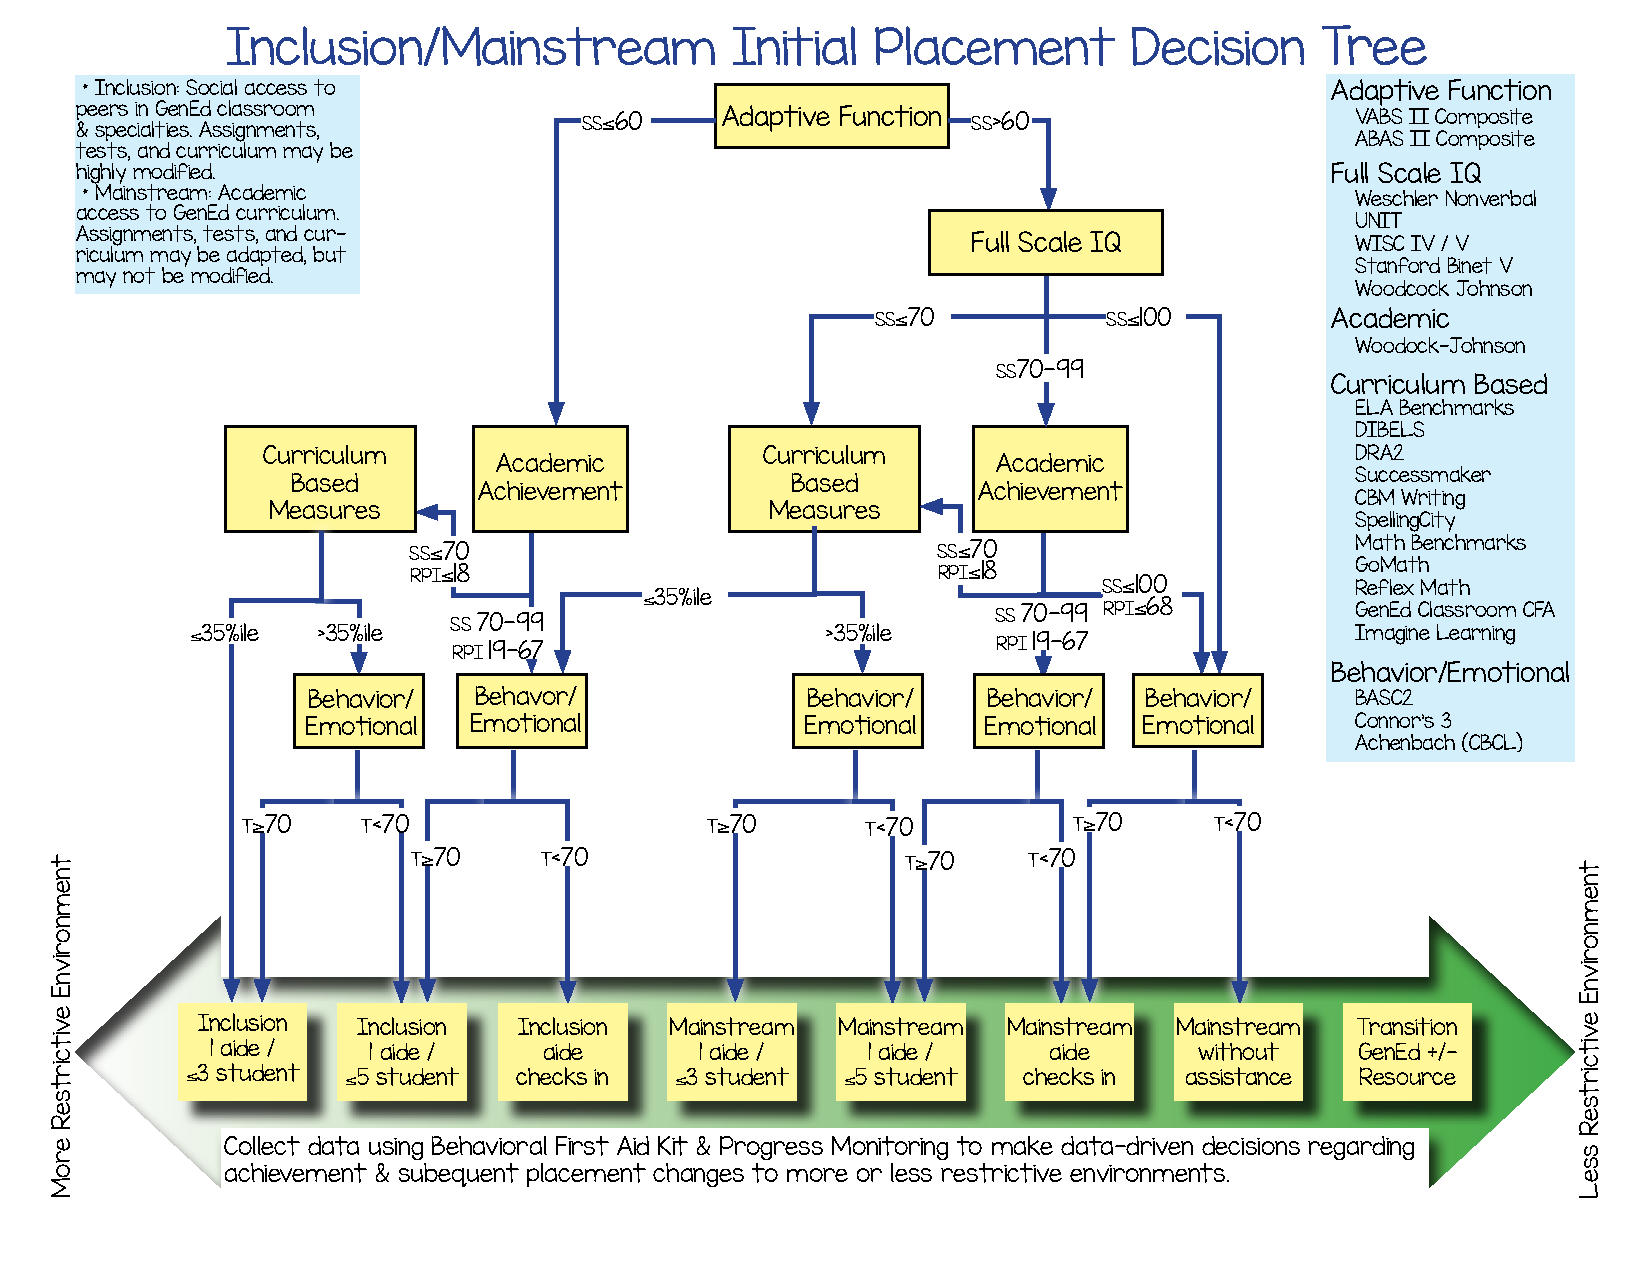
\includegraphics[width=\textwidth]{Figure1.pdf}
\caption[Mainstreaming Decision Tree]{\textit{Mainstreaming Decision Tree. The Mainstreaming Decision Tree is a visual depiction of the data-driven decision making process used to identify candidates for transition from self-contained special education to general education with part time special education/Resource services placements. Data regarding Adaptive Function is the first decision point, followed by Full Scale IQ, Academic Achievement, and Socio-Emotional Well Being. Along the bottom are the spectrum of restrictive environments ranging from inclusion with an aide on the left to independent mainstream access to the general education classroom on the right.}}
\label{fig1}
\end{figure}
%
%%%%%%%%%%%%%%%%%%%%%%%%%%%%%%%%%%%%%%%%%%%%
%
% End Figure 1
%
%%%%%%%%%%%%%%%%%%%%%%%%%%%%%%%%%%%%%%%%%%%%
%
%%%%%%%%%%%%%%%%%%%%%%%%%%%%%%%%%%%%%%%%%%%%
%
% End of Chapter
%
%%%%%%%%%%%%%%%%%%%%%%%%%%%%%%%%%%%%%%%%%%%%
%
\clearpage
%
\chapter[Neuropsychological Measures]{Hierarchy of Measures Included in Mainstream Decision Tree}
Table~\ref{tab1} contains all the data types input into the \textit{Mainstream Decision Tree}. Table~\ref{tab2} identifies data types explicitly \textit{excluded} from the decision making process as these were judgment calls informed by personal and professional biases. Finally, Table~\ref{tab3} provides research based cutoff scores that serve to predict student success in the general education classroom.

The hierarchy followed by the \textit{Mainstreaming Decision Tree} is Adaptive Function as the first decision point, followed by Full Scale IQ, Academic Achievement, and finally Socio-Emotional Well Being. These items were placed in this order to maximize predictive validity of the process by emphasizing certain measures at earlier or later stages of decision making. The flow of decision points can be seen in Figure~\ref{fig1} looking from top to bottom.

Important for understanding the intent of the \textit{Mainstreaming Decision Tree} is the difference between inclusion and mainstreaming. The operational definitions used in the \textit{Mainstreaming Decision Tree} and \textit{Mainstreaming Pipeline} are as follows. Inclusion refers to \textit{social} access to peers in a general education classroom. Assignments are often highly modified for inclusion (assignment modification means entirely different materials or assignments that reduces the expectations on student achievement or alteration to the required curriculum). Mainstreaming refers to \textit{academic} access to the general education classroom. Assignments, tests, and curriculum have to be the same as  general education peers or slightly adapted/accommodated (meaning the expectations for achievement and curriculum requirements remain the same, but the assignment can be changed by response mode or reduction of work load to facilitate student success), but cannot be modified. 

\section[Neuropsychological Measures]{Adaptive Function}
Adaptive Function was chosen as the first decision point because of its pivotal role in behavioral flexibility in novel situations. Adaptive function is an individual's competence of social and practical daily living skills \footcite{de2005adaptive,ditterline2008adaptive,gresham1987relationship}. Adaptive skills are necessary for an individual to adjust their behavior to novel situations or contexts (\textit{i.e.}, change inappropriate behaviors to more appropriate ones given a situation). Adaptive function was emphasized because it underlies the practical, everyday skills needed to function and meet the demands of an individual's environment, including the skills necessary to effectively and independently take care of oneself and to interact with other people \footcite{oakland2011adaptive}. These adaptive skills are crucial to achieving success in a general education classroom environment. 

Having adaptive function as the first decision point makes the \textit{Mainstreaming Decision Tree} conservative so far as taking student coping skills and adaptability into account. Low adaptive composite standard scores result in placing the student in more restrictive settings with increased behavioral and academic supports. Once the student responds favorably to these supports, the student progresses to increasingly less restrictive educational settings. 

\section[Neuropsychological Measures]{Cognitive/Intellectual Abilities}
Intellectual Abilities (Full Scale IQ) were given lower priority relative to adaptive function simply because a low IQ can be unduly influential if included as the first step of a decision making process. Decades of research suggest IQ measures can be poor predictors or correlates of cognitive ability and success in developmentally disabled populations that are well represented in special education classrooms (\textit{e.g.}, spina bifida, autism, and 22q11.2DS; \footcite{biswas2016cognitive,dennis2009iq,popa2014atypical,nader2014does}). In fact, it has been demonstrated over and over that there is a bias in IQ tests, with some underestimating the cognitive ability more than others\footnote{\textbf{\textit{CITE MICHELLE DAWSON'S WORK}}}

IQ tests measure an individual's cognitive faculties of intellect in comparison to others. The results of IQ tests are proxy to the mental agility of a person. Importantly, intelligence does not cause academic achievement, it simply correlates with achievement \footcite{konold1997factor,wechsler2008wechsler}; or, in some cases, FSIQ values fail to correlate with an individual's ability to be successful \footcite{biswas2016cognitive,dennis2009iq,popa2014atypical,nader2014does}.

\section[Neuropsychological Measures]{Academic Achievement}
Academic Achievement was chosen to be the next decision step. We focus on the Woodcock-Johnson III NU (WJ-IIINU) because it was the primary tool to assess academic achievement in our school district at the time of this writing. However, the use of appropriate curriculum based measures often gives a more complete snapshot of academic achievement by directly measuring academic skills in the classroom \footcite{mathes1998preparing}. Specifically, with the increasing prevalence of grade-wide common formative assessments (CFA) in the general education classroom, these can be even more reliable indicators of success than standardized achievement tests \footcite{dunn2009critical,heritage2007formative,mathes1998preparing}. As such, curriculum based measures were given priority over achievement scores from the WJ-IIINU.

The WJ-IIINU Tests of Achievement were widely used to assess students for learning disabilities and the resulting data were useful for determining if the students qualify for specialized services. The WJ-IIINU Tests of Achievement uses clusters of tests that directly parallel critical learning goals outlined by IDEA and provide sound procedures for determining discrepancies between student potential and achievement. Curriculum based measures used as direct measure for classroom performance relative to peers in general education environment \footcite{edwards2006factorial,taub2004confirmatory,wu2008short}.

\section[Neuropsychological Measures]{Socio-Emotional Well Being}
Socio-Emotional Well Being is the final decision point in the \textit{Mainstreaming Decision Tree}. This was intended to quantify anxiety and/or emotional self regulation that deleteriously impact classroom performance. Behavioral and conduct problems that require behavioral intervention can be considered as well at this step (\textit{e.g.}, Behavioral Symptoms Index (BSI) on the BASC-2/3 or Conduct Problems on the Connors 3 and/or Achenbach CBCL). These data were included because behavioral and emotional functioning of children and adolescents can be effective measures for predicting student success \footcite{wiesner2013exploratory}. 

Academic problems, along with problems associated with developing and maintaining positive relationships with others, are often the result of underlying behavioral and emotional challenges. These challenges, when identified and addressed sufficiently early, can be corrected before negatively affecting a child or adolescent \footcite{raines2012universal,reid2004meta}.

The decision to place Socio-Emotional Well Being as the final decision step was deliberate. Once the other factors have been accounted for in the decision making process, this step modulates earlier decisions by placing the student in either a slightly more or less restrictive environment based upon their anxiety and/or behavioral profiles. In other words, Socio-Emotional Well Being was used explicitly to provision increased support for the student if needed to prevent student perception of being overwhelmed by the level of challenge in the classroom. The working model used to describe the role of anxiety of behavioral disorders on student success was based on the Yerkes-Dodson inverted U Law (\textit{cf.}, Figure~\ref{fig2}; \footcite{yerkes1908relation,cohen2011yerkes,cooray2005anxiety}).
%
%%%%%%%%%%%%%%%%%%%%%%%%%%%%%%%%%%%%%%%%%%%%
%
% Begin Figure 2
%
%%%%%%%%%%%%%%%%%%%%%%%%%%%%%%%%%%%%%%%%%%%%
%
\begin{figure}[htp!]
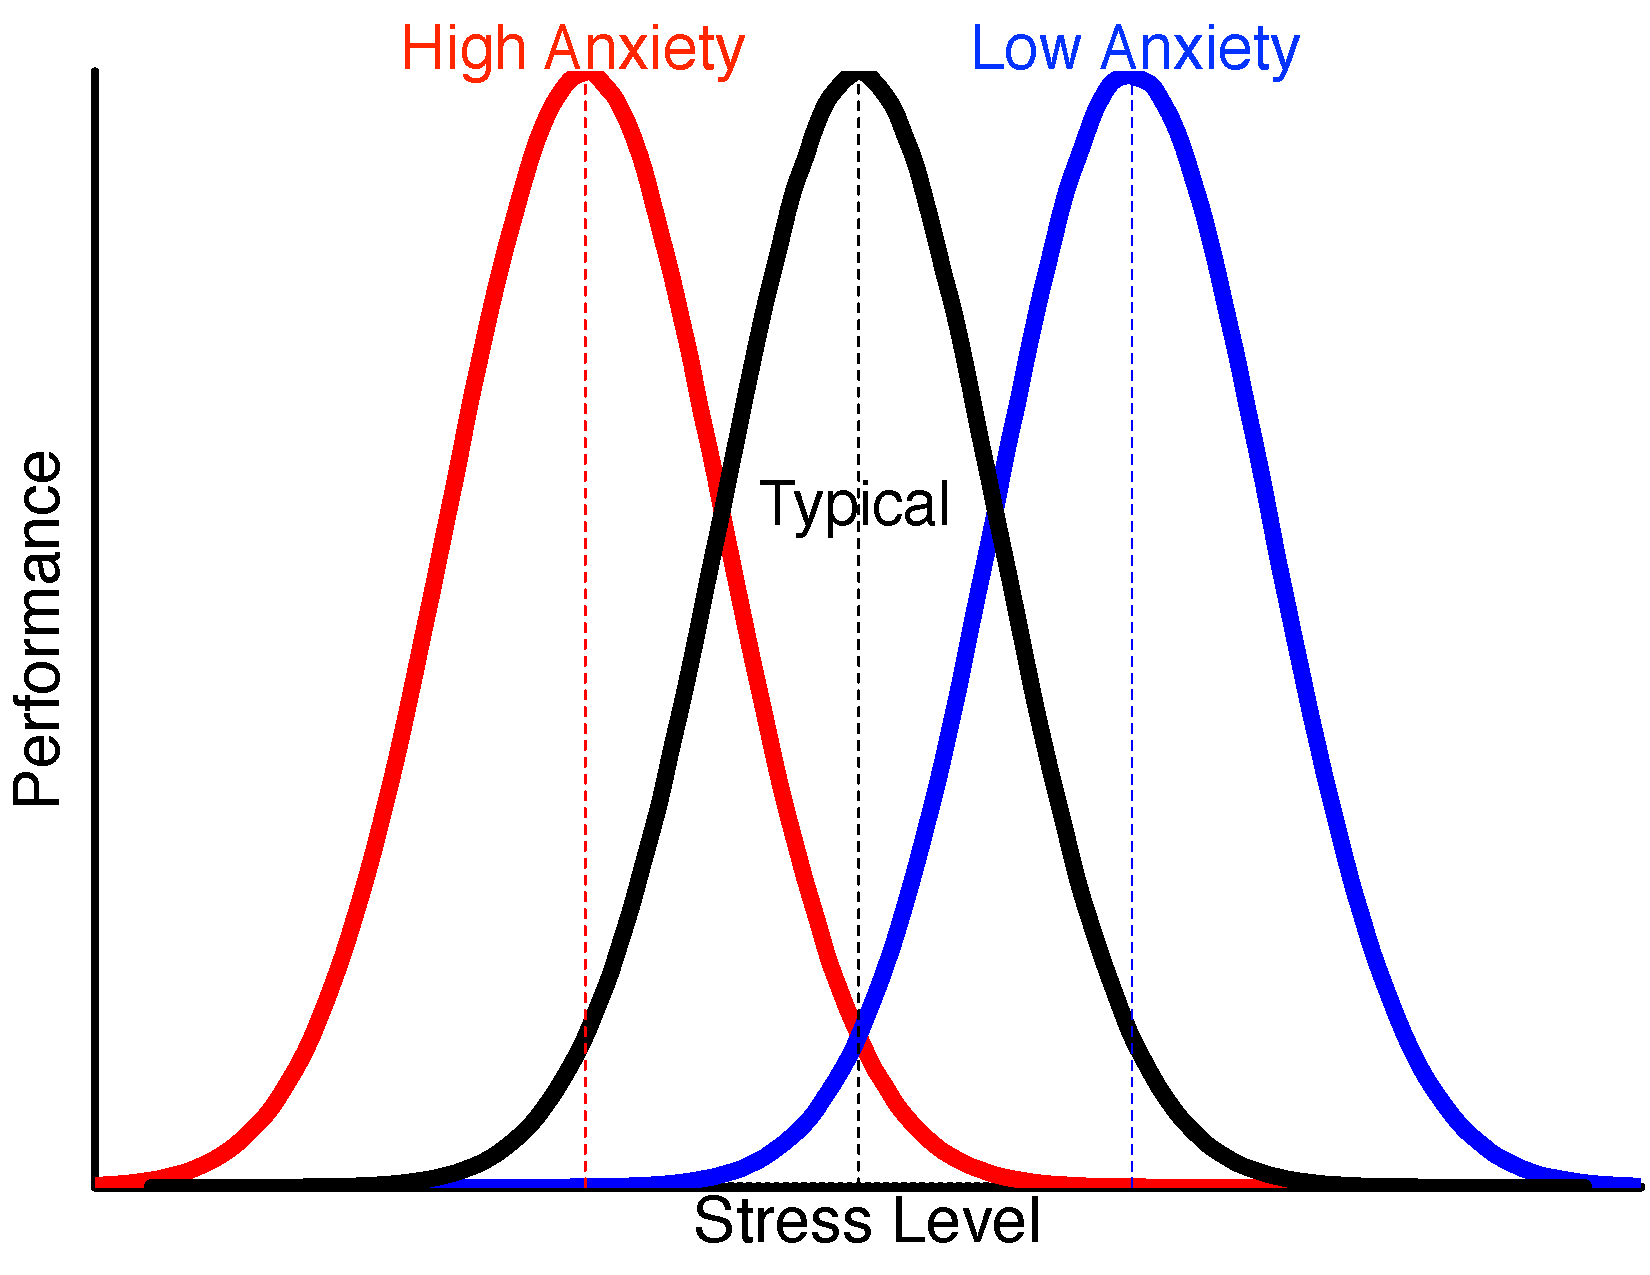
\includegraphics[width=\textwidth]{Yerkes-Dodson.pdf}
\caption[Yerkes Dodson Law]{\textit{Yerkes Dodson Law applied to anxiety after \footcite{yerkes1908relation}. There was a clear relationship between stress and performance, with more stress (or challenge) being required to increase performance up to a point. After that point, there was too much stress and performance decreases. The middle curve line is a model curve for a "typical" student. The high anxiety student line (\textit{e.g.}, T\textsubscript{anxiety}\textgreater70 on BASC 2) shows that student performance peaks at lower stress levels. This suggests the students need increased support to shift the curve rightward where the typical curve is located. Low anxiety student performance peaks at higher stress levels. This suggests they need to be pushed and challenged to shift the curve leftward to where the black curve was located, as they are showing poor performance at "typical" levels of perceived stress.}}
\label{fig2}
\end{figure}
%
%%%%%%%%%%%%%%%%%%%%%%%%%%%%%%%%%%%%%%%%%%%%
%
% End Figure 2
%
%%%%%%%%%%%%%%%%%%%%%%%%%%%%%%%%%%%%%%%%%%%%
%
\section[Neuropsychological Measures]{Initial Mainstreaming Placement}
Whether to place the student in a more or less restrictive environment is the result of the \textit{Mainstreaming Decision Tree}. As seen in Figure~\ref{fig1}, the \textit{Mainstreaming Decision Tree} results in candidate placements for inclusion or mainstreaming and suggests a level of restrictive environment that will be appropriate for each student. As students exhibit increased independence, academic and behavioral supports can be gradually faded back, resulting in movement toward a less restrictive environment (\textit{i.e.}, toward full independence in the general education classroom). 

Fading back supports is done in two phases, behavioral and academic-with behavioral scaffolds being released first. For both academics and behavior, the first step is to fade supervision based on least restrictive environment. This means reduced access to inclusion para-educators until the student achieves independence. The next step was to provide specific incentives for continued academic success and behavioral successes. 

If students require greater supports in order to be successful, then more supports and scaffolds can be added, moving the student into more restrictive environments that requires less student independence. To scaffold behavioral success, the first step is to provide incentives to build on achieved successes. Then, if necessary, provide behavioral support in the form of a paraprofessional. These supports can take the form of social skills, emotional, or behavioral interventions. 

To provide academic scaffolds, the first step is to provide incentives for continued academic success. If needed, assignments are adapted (assignments are still never modified). Finally, pull-out or push-in academic services are provided to bridge gaps as needed.
%
%%%%%%%%%%%%%%%%%%%%%%%%%%%%%%%%%%%%%%%%%%%%
%
% Begin Table 1
%
%%%%%%%%%%%%%%%%%%%%%%%%%%%%%%%%%%%%%%%%%%%%
%
\begin{table}[tbp]
\centering
\vspace*{0cm}\caption{Data Considered by a Mainstream Decision Tree}
\label{tab1}
\resizebox{\textwidth}{!}
{\begin{tabular}{ccccc}
\hline\\[-1.5ex]
Adaptive & Intelligence & \multicolumn{2}{c}{Academic Achievement} & Emotional \\[0.5ex]
\cmidrule(lr){3-4}
 & & Woodcock Johnson IIINU/IV & Curriculum Based Measurements & \\
\hline\\[-1.5ex]
VABS 2/3 & Stanford Binet V & Reading Skills & District Benchmarks & BASC 2/3\\
ABAS 2/3 & Weschler Nonverbal & Reading Comprehension & Utah Compose & Connor's 3\\
BASC 2/3 (Adaptive) & WISC IV/V & Math Calculation & AIMS Web & Achenbach CBCL\\
 & Woodcock Johnson IIINU/IV & Math Reasoning & DRA 2 & \\
 & KBIT 2 & Broad Writing (includes Spelling) & Spelling City & \\
 & Leiter R & Broad Reading & GoMath Benchmark, Chapter Tests & \\
 & UNIT 2 & Broad Math & Eureka Math &\\
 & & & DIBLES Next &\\
 & & & Success Maker &\\
 & & & Imagine Learning &\\
 & & & Reflex Math &\\
 & & & Common Formative Assessments (CFA) &\\
 & & & \textbf{Any evidence-based measure approved by IEP team} &\\
\hline
\end{tabular}}
\end{table}
%
%%%%%%%%%%%%%%%%%%%%%%%%%%%%%%%%%%%%%%%%%%%%
%
% End Table 1
%
%%%%%%%%%%%%%%%%%%%%%%%%%%%%%%%%%%%%%%%%%%%%
%
%%%%%%%%%%%%%%%%%%%%%%%%%%%%%%%%%%%%%%%%%%%%
%
% Begin Table 2
%
%%%%%%%%%%%%%%%%%%%%%%%%%%%%%%%%%%%%%%%%%%%%
%
\begin{table}[tbp]
\centering
\caption{Data \textit{Not Considered} by a Mainstream Decision Tree}
\label{tab2}
\begin{tabular}{l}
\hline\\
Behavioral data from the self-contained classroom\\
Past lack of success in mainstreaming\\
Past lack of school skills necessary for mainstreaming\\
Anecdotal reports of any kind not supported by data\\
Requirement for para-educator time or resources\\
Student idiosyncrasies/peculiarities\\
Student personality\\
Parent concerns about academic abilities\\
Parent concerns about behavioral abilities\\
Social skills deficits\\
Student mobility issues\\
Special education classification\\
Student speech issues\\
Information regarding disability\\
Medical/Psychiatric diagnoses\\
~~~~~Autism\\
~~~~~ADHD\\
~~~~~Epilepsy\\
~~~~~Tic Disorders\\
~~~~~Tourette's\\
~~~~~ODD, OCD, Bipolar, BPD, etc.\\
~~~~~Anxiety/Depression status \\
Current or past medications\\
Hesitation of parents to pursue psychiatric help for student\\
Medication compliance or noncompliance\\
Quality of Relationship Teacher has with Parent\\
"Red Flag" or helicopter parent \\
\hline
\end{tabular}
\end{table}
%
%%%%%%%%%%%%%%%%%%%%%%%%%%%%%%%%%%%%%%%%%%%%
%
% End Table 2
%
%%%%%%%%%%%%%%%%%%%%%%%%%%%%%%%%%%%%%%%%%%%%
%
%
%%%%%%%%%%%%%%%%%%%%%%%%%%%%%%%%%%%%%%%%%%%%
%
% Begin Table 3
%
%%%%%%%%%%%%%%%%%%%%%%%%%%%%%%%%%%%%%%%%%%%%
%
\begin{table}[tbp]
\centering
\caption{Cutoff/Criteria Performance Levels for Mainstream Decision Tree}
\label{tab3}
\begin{tabular}{cc}
\hline \\
Adaptive & Intelligence\\
\hline \\
VABS II/3 or ABAS II/3 & Any FSIQ, NVIQ, or VIQ Measure\\
SS \textless60 & SS \textless70\\
SS \textgreater60 & SS 70-100\\
BASC 2/3 (Adaptive) & SS \textgreater100\\
T \textless30 & \\
T \textgreater30 & \\
\hline \\
Academic & Socio-Emotional\\
\hline \\
WJ-IIINU/IV & BASC 2/3/Connor's 3/CBCL\\
SS \textless70 \& RPI \textless18 & T \textless70\\
SS 70-100 \& RPI 18-34 & T \textgreater70\\
SS \textgreater100 \& RPI \textgreater34 &\\
\hline
\end{tabular}
\end{table}
%
%%%%%%%%%%%%%%%%%%%%%%%%%%%%%%%%%%%%%%%%%%%%
%
% Begin Table 3
%
%%%%%%%%%%%%%%%%%%%%%%%%%%%%%%%%%%%%%%%%%%%%
%
%
%%%%%%%%%%%%%%%%%%%%%%%%%%%%%%%%%%%%%%%%%%%%
%
% End of Chapter
%
%%%%%%%%%%%%%%%%%%%%%%%%%%%%%%%%%%%%%%%%%%%%
%
\part{Implementing the Solution}
%
\chapter[Mainstreaming Pipeline]{Development of a \textit{Mainstreaming Pipeline}}
Once candidate students were identified and placed in an appropriate setting for inclusion/mainstreaming using the \textit{Mainstreaming Decision Tree}, then a specific transenvironmental programming process needs to put into place to guide students toward success in increasingly less restrictive environments. This pipeline was designed to simultaneously build student confidence and ability by stretching and challenging them both academically and behaviorally while providing sufficient scaffolds and support to prevent student failure. To achieve effective transenvironmental programming methods, we developed a 7-step \textit{Mainstreaming Pipeline} based on previous research\footcite{fuchs1993conservative,fuchs1994classroom,marden2013criteria,mathes1998preparing,wadsworth1999preparing,wadsworth1999preparing}. 

\section[Pipeline]{Step 1 - Identify Candidate Students}
As described above, candidate students were identified with the \textit{Mainstreaming Decision Tree} using broad Adaptive scores (Adaptive Composite Standard Score from ABAS-II/ABAS-3 or VABS-II/VABS-3 or else adaptive T-score on BASC2/3), Full Scale IQ (or NVIQ/VIQ as appropriate), Academic Achievement (CBM/CFA or WJ-IIINU/IV), and Socio-Emotional Well Being. To do this, a copy of the \textit{Mainstreaming Decision Tree} was printed off and a highlighter was used to trace down the decision points for each student individually to identify initial inclusion/mainstreaming placement options. The values at each decision point were annotated in a Mainstreaming Data Sheet (form available as Appendix~\ref{Appendix2})

Note, not at this point nor at any other point moving forward were special education classification, medical diagnoses, mobility problems, speech issues, or anything else included in Table~\ref{tab2} considered as factors. Neither did teachers consider past difficulties in mainstreaming except as motivation for the development of behavioral plans to scaffold student success. The final element within this step was to write a very precise description of each student in terms of temperament and relative need for structure compared to peers (both compared to special education and general education peers).

\section[Pipeline]{Step 2 - Identify Classroom Placements}
Once candidate students are identified, it becomes critical to identify grade level classrooms as placement options. There are two approaches to doing this: First, one can identify teachers with a known history of working with special education. Second, one can refrain from limiting candidate classrooms to any given teacher, but look at all grade level classrooms to determine best placement options on a student by student basis.

The preferred option is to evaluate all grade level classrooms as candidate placements. This prevents issues associated with the special education department overwhelming a relatively small number of teachers with extra students while not impacting other classrooms within the school \textit{\textbf{[PUT IN REFERENCES HERE]}}. Any teacher-student personality considerations based on the profile completed in Step 1 should be addressed with the building administrator prior to moving forward with any placements. 

\section[Pipeline]{Step 3 - Classroom Ecological Inventory}
This step involves harmonizing the special education and general education environments to maximize the potential for student success. It was based strongly on the evidence based transenvironmental programming methods employed by the Peabody Reintegration Project and refined by Fuchs and colleagues \footcite{fuchs1993conservative,fuchs1994classroom,marden2013criteria,mathes1998preparing,wadsworth1999preparing,wadsworth1999preparing}. 

The components to this Classroom Ecological Inventory process are as follows: 

\subsection[Pipeline]{Component 1} Special education teacher (or district facilitator/coordinator) observes candidate general education classrooms to identify any issues that will limit success as well as identify classroom factors that will increase probability of student success. 

\subsection[Pipeline]{Component 2} The special education and general education teacher independently complete a shared ecological inventory for their classrooms that can be used to identify any discrepancies in classroom environment that may impact student success (modified after previous reports \footcite{fuchs1994classroom,marden2013criteria}). In other words, the special education and general education teachers describe their classroom environment, expectations, management styles, etc. This form is available as Appendix~\ref{Appendix4}.

\subsection[Pipeline]{Component 3} Any discrepancies in the teachers' responses to the inventory were identified and discussed to identify potential difficulties for the student moving forward.

\subsection[Pipeline]{Component 4} The teachers discuss plans/solutions to potential difficulties for the student based on the data from the ecological survey. The most common issues observed were increased rigor of curriculum in general education compared to special education, insufficient student independence, and different curricula between special education and general education. The most commonly proposed solutions were planned accommodation of assignments (to be faded over time), increasing academic rigor in the special education classroom, and special education classrooms increasing homework load prior to the transitions so the student develops the academic skills required by homework. 

\subsection[Pipeline]{Component 5} The special education and general education teachers specifically plan classroom accommodations for moving forward. This step involves a number of informal meetings and an in depth conversation as to precise expectations regarding student performance in the general education classroom. 

Critically, there can be no assignment modification during any step of the mainstreaming process. Assignments can be adapted so the student can access the curriculum (\textit{e.g.}, change response mode or reduce total work load), but no expectations for curriculum or content mastery can be reduced. Such modifications impede long term transition out of special education, whereas appropriate accommodations increase the probability of future success \footcite{fisher2003special,fuchs2003responsiveness,hollenbeck1998teachers}.

\section[Pipeline]{Step 4 - Initiate Student Placement in General Education Classroom}
The \textit{Mainstreaming Decision Tree} can be used to identify the specific needs of the student for support levels. At this time need for para-educator allocation and student specific behavior plans is discussed. The student is placed in the general education classroom for ~50\% time to begin (unless the IEP team decision was to start with a greater percentage of time).

Upon beginning to attend the mainstream classroom, the special education teacher begins data collection on student independence using a Mainstreaming Data Sheet (Appendix~\ref{Appendix2}). Data collection on independence, levels of accommodation necessary for student success, and classroom behavior were also collected by a district facilitator/coordinator. Behavioral data sheets used during this implementation are available as digital files by request or at the end of this book as Appendix~\ref{Appendix5}

\section[Pipeline]{Step 5 - Transition from Part-Time to Full-Time General Education}
Student time is increased in the general education class until they independently participate 90-100\% of the time in the general education classroom and/or Resource classroom \textit{prior to} moving toward a re-evaluation/placement change. Any increases of student time in general education classroom or movement in the direction of transitioning toward change of placement are based on the following factors: 1) Independence as quantified by a Mainstreaming Data Sheet, 2) Classroom observations, 3) Work completion, and 4) Academic progress, primarily referring to how much accommodation the student needs (\textit{i.e.}, whether or not the student completes coursework with the same assignments as peers receiving only part time special education/Resource services). This final criteria is important because the majority of students transitioning out of self-contained classrooms will need part time special education/Resource services to achieve success.

\section[Pipeline]{Step 6 - Formal Transition from Special Education to General Education}
The IEP team performs a data review to determine how to proceed with a change of placement. Additional academic testing can be administered (\textit{e.g.},WJ-IIINU/IV) as part of a re-evaluation to illuminate present levels of academic functioning and performance if CBM benchmarks and CFA performance were insufficient. These results guide IEP goal development and to ascertain appropriate levels of part time special education/Resource services.

During this transition, the IEP team develops all necessary behavior plans, contracts, trackers, etc. Any plans or contracts must be designed to fit seamlessly into the school PBIS framework or other school-wide discipline system.

\section[Pipeline]{Step 7 - Transition from Unit School to Neighborhood School}
At the end of the year, there should be a transition meeting with the student's neighborhood school to discuss necessary accommodations, successes, challenges, etc. The following issues need to be discussed: 1) Transition plans: decisions need to be made whether the student returns to their neighborhood school or stay at the school wherein they attended the self-contained classroom. 2) Staffing issues across both schools: It is imperative the schools verify that the impact of any given student or group of students transitioning from one environment to another will not overwhelm individual teachers or grade levels the subsequent year. However, staffing at a particular school is insufficient reason to restrain decisions involving moving students back to their neighborhood schools. This was a discussion among the building administrators of the individual schools (not the teachers). Finally, 3) What transitional assistance the next school year by district facilitator/coordinator should look like.

The two school teams need to develop a set of transitional IEP goals to scaffold the student into a new school/grade/placement, preferably with goals geared toward full student independence in the general education classroom. Additionally, there needs to be a conversation regarding how often a district facilitator/coordinator explicitly checks in on transitioned students at their new school.
%
%%%%%%%%%%%%%%%%%%%%%%%%%%%%%%%%%%%%%%%%%%%%%
%
% End Chapter
%
%%%%%%%%%%%%%%%%%%%%%%%%%%%%%%%%%%%%%%%%%%%%
%
\clearpage
%
\chapter[Behavioral Decision Tree]{Behavioral Mainstreaming Decision Tree}
Once academic decisions have been made using the \textit{Mainstreaming Decision Tree}, it becomes necessary to quantify the behavioral needs of the students. To accomplish this, I created a \textit{Behavioral Mainstreaming Decision Tree} (Figure~\ref{fig3} and Appendix~\ref{Appendix2}). This was designed for mainstreaming decisions for students in SocioEmotional Learning/Emotional Disturbance/Behavior classrooms. 

Similarly to how the academic \textit{Mainstreaming Decision Tree} relies on data rather than teacher or student judgment, the\textit{ Behavioral Mainstream Decision Tree} focuses on behavioral data easily collected by the classroom teacher and validated by other staff as fidelity checks. 

The first component of the \textit{Behavioral Mainstream Decision Tree} is whether the behavior of the student requires the use of seclusionary time out/Time Out Booth or Physical Restraint (also called Forced Physical Guidance and Manual Restraint in some LEAs). The use of these emergency safety interventions is limited in most areas to instances where the behavior fo the student is an \textit{immediate and significant danger} to themselves or other. If a student requires the use of these interventions,they require instruction in social skills and socio-emotional self regulation prior to attempting any mainstreaming or social inclusion. 

The second component of the \textit{Behavioral Mainstreaming Decision Tree} is whether the student engages in Physical Aggression. Importantly, this does not include property destruction. A student destroying property and a student attacking another person are very different things and should not be confounded. Physical Aggression includes punching, kicking, slapping, headbutting, using chairs, pencils, etc as weapons to hit another, spitting on, or biting another person. 

Importantly for this component, I differentiate between a physical aggression even if the student was provoked by another student or teacher in the room and those when the student aggresses without clear provocation. Provocation in this sense includes peers or adults making physical contact with a student or restricting their movement. Similarly, using "fighting words" to escalate a student or specifically trigger them is considered provocation. 

The third decision point is that of inappropriate vocalizations. If a student engages in \textit{pervasive} inappropriate language or vocalizations they  will be considered for a more restrictive mainstreaming placement compared to if they do not. For this decision point, inappropriate vocalizations include very specific things: they include screaming used to back off adults or teachers. They also include using specifically course and vulgar language. For clarity, this means if a student is generally talking about Slenderman or killing or hurting someone that \textit{does not} count as an inappropriate vocalization so long as it is not a credible threat. If a student uses words like damn, shit, bitch, bastard, fart, poop, etc. I do not count these, regardless the community standards. If stduents use words like fuck, shit, cunt, cock, sexually accurate descriptions of sex organs, descriptions of rape, etc I do consider these inappropriate vocalizations. I draw this line where I do as the latter vocalizations do not tend to go away in a new environment. The former do.

Similarly to the Mainstreaming Decision Tree, the next component is to choose the level of support necessary for mainstreaming. Meetings should happen biweekly to determine if a more or less restrictive environment is necessary for student success.  As students exhibit increased independence, academic and behavioral supports can be gradually faded back, resulting in movement toward a less restrictive environment (\textit{i.e.}, toward full independence in the general education classroom). 

Fading back supports is done in two phases, behavioral and academic-with behavioral scaffolds being released first. For both academics and behavior, the first step is to fade supervision based on least restrictive environment. This means reduced access to inclusion para-educators until the student achieves independence. The next step was to provide specific incentives for continued academic success and behavioral successes. 

If students require greater supports in order to be successful, then more supports and scaffolds can be added, moving the student into more restrictive environments that requires less student independence. To scaffold behavioral success, the first step is to provide incentives to build on achieved successes. Then, if necessary, provide behavioral support in the form of a paraprofessional. These supports can take the form of social skills, emotional, or behavioral interventions. 

To provide academic scaffolds, the first step is to provide incentives for continued academic success. If needed, assignments are adapted (assignments are still never modified). Finally, pull-out or push-in academic services are provided to bridge gaps as needed.

Critically, if the two different decision trees (academic and behavioral) result in different levels of restrictive environment, the teams will meet to harmonize the differences between the results and what placement is in the best interest of the students. 
%
%%%%%%%%%%%%%%%%%%%%%%%%%%%%%%%%%%%%%%%%%%%%
%
% Begin Figure 3
%
%%%%%%%%%%%%%%%%%%%%%%%%%%%%%%%%%%%%%%%%%%%%
%
\begin{figure}[htp!]
	\centering
	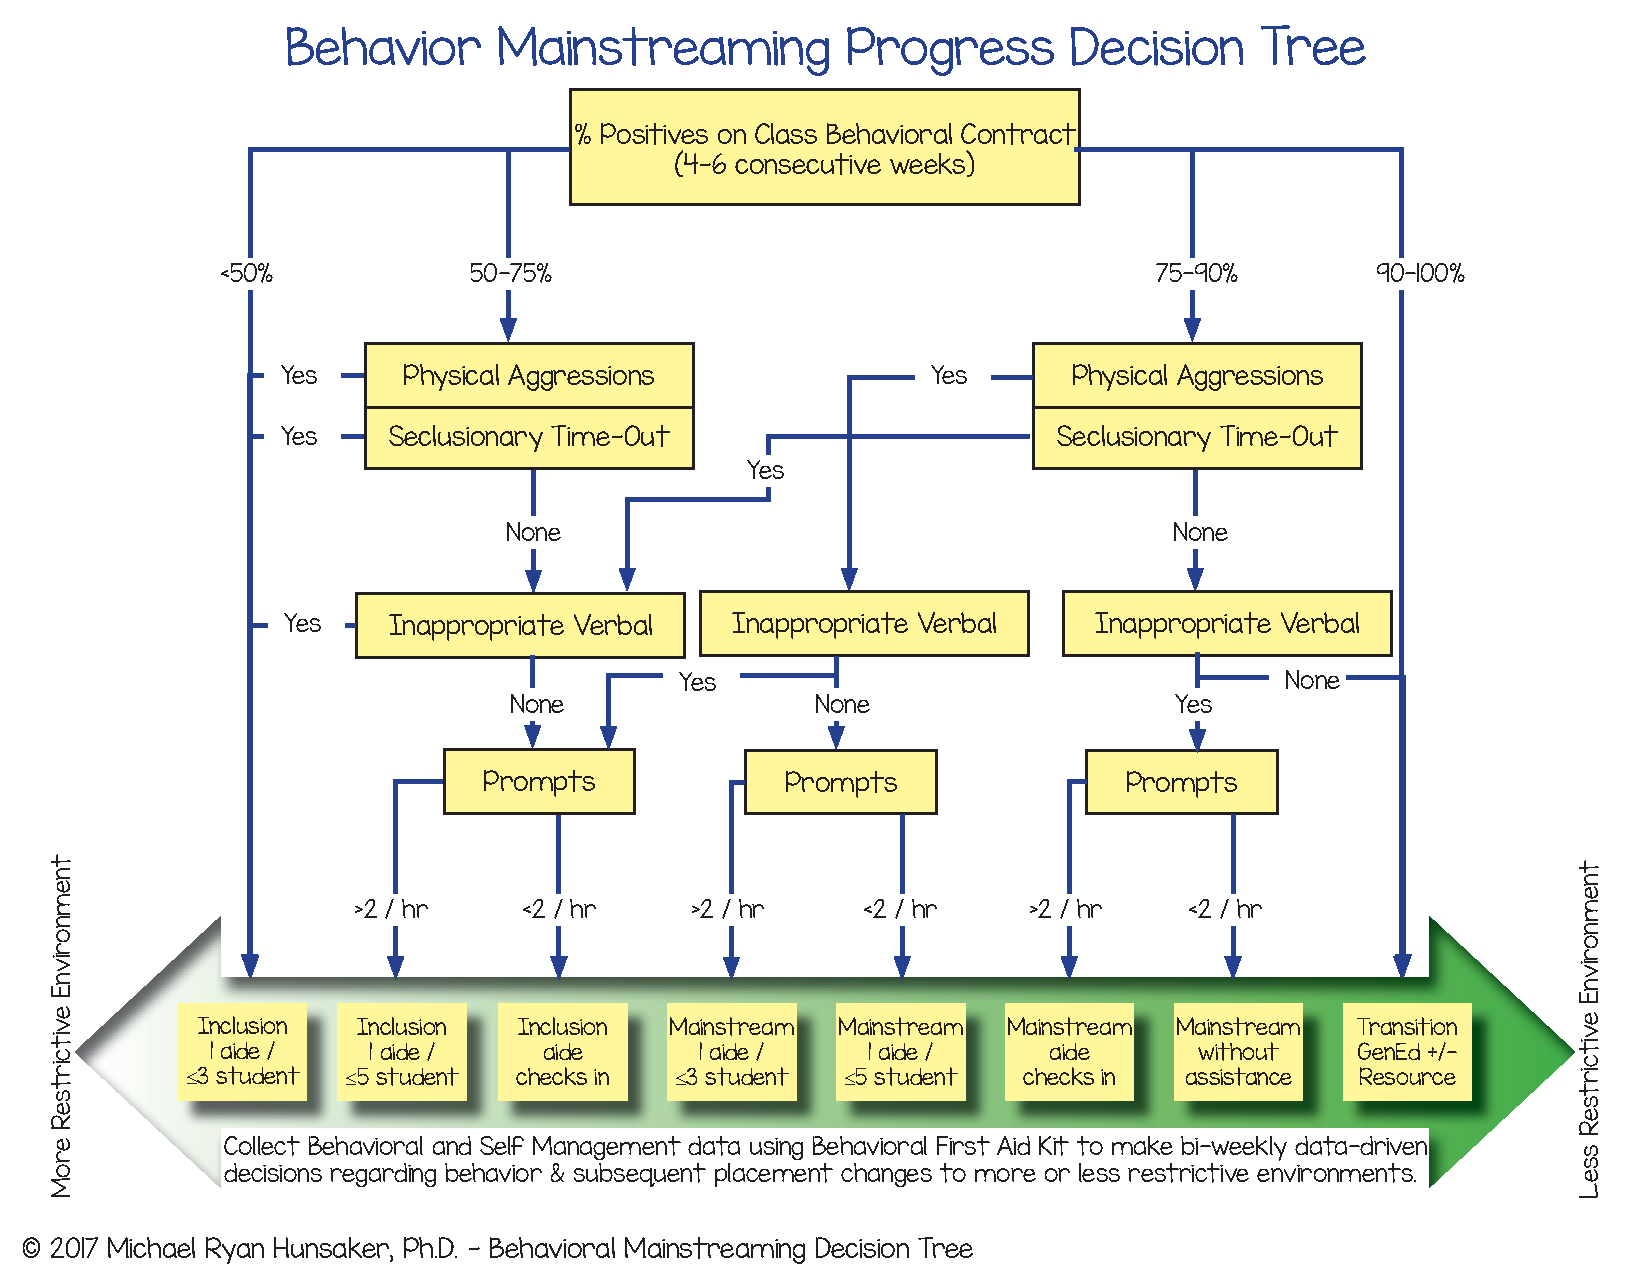
\includegraphics[width=\textwidth]{BehaviorPipeline.pdf}
	\caption[Behaviroal Mainstreaming Decision Tree]{\textit{Behavioral Mainstreaming Decision Tree. The Behavioral Mainstreaming Decision Tree is a visual depiction of the data-driven decision making process used to identify candidates for transition from self-contained special education to general education with part time special education/Resource services placements. Data regarding behavioral performance in self contained and general education classroom are collected and taken into account. Biweekly meetings are held to determine if student needs more or less restrictive environments. Along the bottom are the spectrum of restrictive environments ranging from inclusion with an aide on the left to independent mainstream access to the general education classroom on the right.}}
	\label{fig3}
\end{figure}
%
%%%%%%%%%%%%%%%%%%%%%%%%%%%%%%%%%%%%%%%%%%%%
%
% End Figure 3
%
%%%%%%%%%%%%%%%%%%%%%%%%%%%%%%%%%%%%%%%%%%%%
%
%%%%%%%%%%%%%%%%%%%%%%%%%%%%%%%%%%%%%%%%%%%%%
%
% End Chapter
%
%%%%%%%%%%%%%%%%%%%%%%%%%%%%%%%%%%%%%%%%%%%%
%
\part[Behavioral Considerations]{Behavioral Considerations}
%
\chapter[Insights...]{Insights on Behavioral Management from Animal Research}

I thought it would be interesting to explain a bit of background on why I approach behavioral management of students the way I do. I seem to have somewhat of a unique perspective because my background focused on rodent \textit{\textbf{and}} human behavior. This means I actually spent 15-ish years of my life doing the type of research that many of the behavioral methods used in classrooms and ABA are actually based on, particularly as related to reward schedules.

\section[Insights...]{My Research Life}

When I was an undergraduate student, I started to work in a rat behavior laboratory as part of a work study program. I ended up spending almost 8 years there. What we were interested in were the roles of different parts of the brain for learning and memory. However, I am actually going to focus on a more mundane part of rodent (and mouse) training: acclimatizing the rats to dealing with humans, other rats, and new situations.

Before we allowed any student to start a behavioral experiment with a rat, they were required to spend 5 days handling the rat and feeding it Froot Loops (our reward of choice) for 15 minutes a day. To do this, there was a very simple shaping process. We started by moving the rat's cage over to the table the new student researcher was sitting at. 

\begin{itemize}
\item \textbf{Step one/Day one} was having the researcher reach into the rat's cage and put their hand in the cage away from the rat. The rat was allowed to come over and sniff the researcher's hand and cuddle up to the warmth. 
\item \textbf{Step two/Day two} was the researcher reaching into the cage and gently grabbing the rat around the midsection, lifting the rat an inch or so, and then letting the rat go. 
\item \textbf{Step three/Day three} involved picking the rat out of the cage and placing it on a lab coat on the researcher's lap. The researcher then kept contact with the rat with at least one hand and basically pet the rat for 15 minutes. 
\item \textbf{Step four/Day four} was identical to Day three. 
\item \textbf{Step five/Day five} involved the researcher picking up the rat and walking around while holding the rat and petting it. Note: The same process works for mice!
\end{itemize}

We found over time that this was an essential step to the success of our research program. If anyone skipped this habituation stage, then the rat would never perform optimally during the experiment. The rats would be impulsive and show a tendency to attack or try to attempt an escape from the researcher. These rats would react poorly (\textit{i.e.}, flip out) when they were touched and would react negatively to noises in lab. Out of curiosity, we quantify this by looking at the mazes and tables after unhabituated rats were finished, the mazes had significantly more rat droppings that stunk something awful and the droppings were not as solid as normal (in layman terms, the rats were scared so they got diarrhea). There was also increased amounts of urine on the mazes as well, which also had a different smell than typical rat urine. We concluded that unhabituated rats were stressed and unable to meet expectations during the behavioral tasks.

I distinctly remember that others in lab were always trying to figure out why my rats were always so smart. They also wondered why I would often perch a rat on my shoulder like a parrot and walk around with a rat nuzzling into my neck. I think it was always a shock when I explained that I had smart rats because they were not anxious or stressed out-in more anthropomorphic terms-they trusted me. At least that was until I had to use aversive stimuli as part of my research. But we will get to that later.

\section[Insights...]{Trust Translates into Motivation}

We had three types of behavioral experiments: 1) Experiments that used Froot Loop rewards to motivate behavior. 2) Experiments that used a rat's natural tendency to explore their environment as intrinsic motivation. And 3) Experiments that used aversive stimulus to condition fear (the shocks were the same experience as touching a 9-Volt battery to your tongue-it was aversive but not painful).

Interestingly, the first two types of experiments, those relying on either positive reinforcement (Froot Loops) or intrinsic reward/motivation (exploration) required the researcher to develop a good relationship with the rat. That is, the 5 day habituation protocol (I called it habituation or snuggle training) was required in order for rats to perform optimally during the tasks. If that period was skipped, even control rats (those that did not have any experimental manipulation done to them) had a very hard time learning the tasks. However, if we helped the rats to trust us, then they were able to do remarkable things.

With trust, we were able to motivate rats to jump across an increasingly large gap between tables, learned to tell the difference between things that were extremely similar, wait a rather long amount of time to respond for reward, and learn rather complicated rules \textit{\textbf{[INSERT REFERENCES HERE]}}. If you clicked any of those links you have guessed that these rats were required to put forth a fair amount of effort to accomplish these tasks. Often times we would watch them and feel a weird sense of pride in the rat stopping at a decision point and looking back and forth before acting-they were thinking \textit{\textbf{[INSERT REFERENCES HERE]}}. They were working hard. And they were rewarded with Froot Loops (and snuggles) for their hard work.

For rats that were part of these first 2 types of experiments wherein the rats either engaged in intrinsically rewarding behavior (exploring) or I rewarded them, there were never any issues with rats trying to escape from the maze or their home cage, brutal self-injury, or attacking other rats, etc. We actually had a few instances wherein a rat escapes it's home cage. We found it curled up asleep in the start box for their experiments. I asked my wife if she had this same experience in the lab and she said she did, her rats were sweethearts that never tried to even bite her. But my wife and I were fastidious about giving each and every rat those first 5 days of habituation and in giving them individualized attention while we were weighing and feeding them. The rats treated us as friends.

\section[Insights...]{Distrust Translates into...?}

When we had student researchers that neglected to handle the rats as we instructed, there was an entirely different profile. The rats were jumpy-as in they would jump out of the cages, the researcher's hands, off mazes, etc. When people walked by the home cages, the rats cowered in the back of the cage and made anxious squeaking noises. These rats were notorious for biting researchers, so the students had to use thick leather or chain mail gloves to handle them. These animals left diarrhea and urine all over the experimental apparatus. These rats tried to jump off the mazes to hide in corners. They attacked other rats and engaged in serious self-injury. In other words, these rats were treating humans as, for lack of a better word, predators. And they were doing what was necessary to intimidate us and to get us to back off, or at least what was necessary to extirpate themselves from the stress of our presence.

Often times, I would have to step in and rehabilitate those rats. We had a strict policy in the research lab that rats were never to be euthanized for aggressive behaviors or in any other way wasted. So, these "tough" rats came onto my docket, because I found out early that I had the patience and ability to work with these difficult animals. My first approach was to do the 5 day habituation session. Even though I was bitten quite a few times during this process, I never got mad at the rat and I definitely never gave up on them. I let the rats realize I was not going to do anything bad to them. Most came around at this point. If there was a rat that did not come around with that shaping, I would more formally write a plan to tame the rat. This usually involved a lot of noncontingent reward (Froot Loops and snuggles). I would crush Froot Loops in my hands and let the rats eat out of my hand and lick the sugar dust off of me. This was irrespective to them biting me. I fulfilled their basic needs, and it worked. They trusted me.

\section[Insights...]{What About That Third Kind of Experiment - Aversive}

This is actually the point of this post. Fear conditioning sucks. Royally.

Here is a typical fear conditioning experimental protocol:
\begin{itemize}
\item A rat is placed in a clear box with a metal rod floor and allowed to explore for 2-3 minutes to learn the layout of the box they are in and see the extra-maze cues.
\item At the end of this period, a 10 second tone comes on, and the last 2 seconds of this tone is paired with a shock. The shock is not painful, but it is rather unpleasant and super-duper scary.
\item Then there is silence for 1 minute and the tone begins-and so on for 8-10 trials.
\item For the next 2 days the rat gets either put in the box in silence for 10 minutes or put in a new box with the tone for 10 minutes to see if they freeze or show fear across days.
\end{itemize}

Clearly, there is absolutely no rewarding component to this experiment. It is pure punishment, and used to study fear pathways and how fear responses develop. I think it goes without saying that these rats are not happy at the end of the experiment.

Well, these rats knew exactly who put them through this cough me. These rats would jump against the cage top and dislodge it to escape. They would aggressively self-mutilate to the point of actually amputating their own limbs! They would posture and attack the side of the cage and lunge at me as I walked by. When I had to get a hold of them, it took all of my skill in handling rats to not get bitten. And many of them left me with scars on my hands that I have to this day.

Many of these rats were loving and calm while running rewarded tasks. When I changed and started providing punishing stimulus, they changed. I did not change what I was doing with regards to giving them attention and calm touches – in fact I increased the noncontingent attention and rewards – but it was never enough. The fact that I was providing or administering punishment was enough to change the researcher-subject dynamic. I punished the rat, so the rat was going to defend itself. I was no longer associated with reward.

\section[Insights...]{Let's Bring This Back to the Classroom}

I am quickly becoming an outspoken critic of response cost and other behavioral management methods that amount to positive and negative punishment because they just do not work. I hear over and over that if there are enough positives then the negatives of a level system are not that bad. I can tell you from experience in rat research (which all these ABA-flavored methods are fundamentally based on), there is no amount of reward I can give (including literal-and liberal-handfuls of Froot Loops in their home cage) that makes up for punishment. What I mean by that is that punishment is infinitely more salient than reward. So, we can give a million gold stars in a day, but all the kid is going to remember from the day that he was moved down from green to yellow.

These ideas are actually supported by research in classroom management by Robert Marzano among many others that demonstrate for typical kids there need to be at least 4-6 positive statements for every negative statement used in a classroom (and that is per child, not per class, so if you correct a student, you need to praise \textit{that} student 6 times). For special education students, the research keeps expanding upon that number, requiring greater and greater numbers of positive interactions for any negative or aversive interaction (the last time I checked the research articles, it was 16:1 ratio). This clearly demonstrates just how influential any negative or punishing comments can be \textit{\textbf{[INSERT REFS HERE]}}.

Negative systems hold kids back. It teaches them that they have to passively conform to adult demands or they get punished. Unfortunately, it also teaches them that the teacher is to be feared. Just like my rats, kids will fight back by yelling, screaming, punching, biting, spitting, running away, hiding, self-mutilation, and so on. Kids cease to be kids and draw into an almost primal state of self-preservation. And it is not their fault. We did it to them. Just like I did my rats.

However, if one runs an exclusively positive classroom management system (which is very, very hard to do), then students will learn. Positive systems provide an atmosphere in which the students are capable of a great many things: 
\begin{enumerate}
	\item They trust teachers. \item They try new things. \item They feel safe enough to ask for help. \item They accomplish what they thought was impossible. \item They believe in themselves.
\end{enumerate}
All of these capabilities combine to make learning a positive experience, and that should be our goal as teachers in the end.
%
%%%%%%%%%%%%%%%%%%%%%%%%%%%%%%%%%%%%%%%%%%%%
%
% End of Chapter
%
%%%%%%%%%%%%%%%%%%%%%%%%%%%%%%%%%%%%%%%%%%%%
%
\clearpage
%
\chapter[Self Management]{Behavioral Data Sheets for Student Self Management}
This chapter comes from my desire to explain what can be done with the set of behavioral data sheets I have included in Appendix~\ref{Appendix5}. I tried to put in a brief description of what each data sheet would be useful for, but I realize now that this may not be sufficient to help teachers use these tools.

In education, we demand that teachers collect lots of data, especially when they are working on some sort of behavioral or academic intervention with students. However, in our training and professional development we are woefully negligent in training teachers in data collection skills. This extends both to general education as well as special education teachers.

I think this is a tragedy and I look forward to contributing a solution. I will try my best to help teachers reading my blog understand the who, what, when, where, and why of taking data. I also hope I can provide somewhat intuitive data sheets to help teachers be able to not only collect necessary data, but also to size up the situation and select (or design) appropriate data tools accordingly.

So, with that in mind, this will be the first in a series of posts meant to highlight some of my more useful data sheets.

\section[Self Management]{My Background in Data}

Before I dive into any little tutorial of how to use my data sheets, I should briefly introduce myself to those of you that only have followed the education side of this blog.

By training I am a behavioral neuroscientist, more specifically a behaviorist/behavioral analyst. In college and for a few years afterward I worked in an experimental psychology lab studying the neurobiology of learning and memory. In this role I was required to develop behavioral tasks to answer questions about the brain, design data sheets that I could use to collect the data from rats on these behavioral tasks, and interpret what those data meant by plotting the data and harmonizing what I saw with the theories of brain function that were present in the field. I also trained high school students and undergraduate students how to collect data and how to interpret it.

My graduate work was with rats, mouse disease models, and human populations evaluating neurodevelopmental and neurodegenerative disease. Again, I had to develop behavioral methods and data sheets for use in human patient populations, mouse, and rat models of Fragile X-associated disorders, autism, Down syndrome, and traumatic brain injury. All this time I also trained college and high school students in how to use data sheets to collect data. After I completed my Ph.D. dissertation\footnote{if you have a lot of time on your hands it can be downloaded for free \url{\textit{\textbf{https://figshare.com/articles/MR_Hunsaker_Dissertation/920218}}}}, I worked on brain development in monkeys and children with autism, mostly by evaluating how their brains developed using MRI techniques. My second job post Ph.D. was to work with mouse models of Down Syndrome. Again, more behavioral tests, more data collection, etc. Somewhere in the graduate school to postdoctoral work timespan I also tinkered around with some MRI and behavioral data from children with 22q11.2DS.

After my second postdoctoral position, I decided to enter the field of education, specifically K-6 special education. I did this because I had been working in different populations receiving special education services, but I felt like I was not making the kind of impact I desired (I wrote about this struggle in Part 1 of this book). My goal was to apply the knowledge of the brain, behavior, development, neuropharmacology, and my skills as a behavioral analyst (read: data collection and interpretation) to directly help students with disabilities succeed in their education.

To that end, I have applied my obsession with data collection and love of interpreting data to help students. I also have striven to share my knowledge of data collection methods and interpretation with anyone that can use the assist (be fair, anyone that will listen).

\section[Self Management]{What is the Behavioral First Aid Kit?}

The Behavioral First Aid Kit (Appendix~\ref{Appendix5}) is a set of data sheets that I made in collaboration with the special education teachers I worked with. My goal was to design a set of worksheets that I could give to the general education teachers to collect intervention data. In this way, we would have the data necessary to know if students qualified for special education services or not. These data sheets cover everything from very simple 5-trial data sheets to behavioral contracts to Antecedent-Behavior-Consequence (ABC) charts and Functional Behavioral Analysis (FuBA) protocols.

The idea was to work as a group, but given I spent approximately 15 years of my life as a scientist and had spent that whole time teaching many high school and college students how to collect data, my special ed team just threw me at the task. They gave me ideas on what problems we needed to address and I went ahead and came up with the solutions.

\section[Self Management]{Behavioral Self Management}

For this application I will refer to eight (8) of the data sheets from the Behavioral First Aid Kit:
%
\begin{itemize}
\item Behavioral Self Reflection Sheet
\item Daily Behavior Rating Report Card
\item Behavioral Chart
\item Good Job Chart
\item Token Chart
\item Response to Intervention Monitoring Graphs
\item Weekly Log
\item Monthly Task Calendar
\end{itemize}
%
\section[Self Management]{What is Behavioral Self Management?}

Behavioral self management is the goal of all behavioral interventions. Technically speaking, behavioral self management it is the ability of a student to discriminate their own behaviors and collect data on themselves. More colloquially, it is the ability of a student to monitor and adjust their own behavior.

To begin this process, the teacher takes the role of manager for student behavior: the teacher collects data and develops a plan with the student to improve their behavior. During these early stages, the teacher provides high levels of feedback and rewards. At this stage the teacher is still collecting all of the data and sharing it with the student after it has been collected.

As the student is able to respond favorably to the plan the teacher is implementing, the teacher starts to fade back their role in directly managing student behavior and collecting the student data. This is where these data sheets come in: they are simple enough that the students can use them with only minimal training and supervision. The teacher will still need to provide some sort of reward based on achieving their behavioral goals (or help the student access natural forms of reward that don't directly depend on the teacher).

The end goal of any self management program is that the student has control over their behavior and they are able to provide their own reinforcement (self praise) or else access reinforcement independent to the teacher (from peers, other adults, etc). This means they have achieved through great effort what most of us take on a daily basis: self control.

\section[Self Management]{Now on to the Datasheets and How to Use Them}

I will go into each datasheets individually and at the end I will wrap them into a coherent plan.

\subsection{Behavioral Self Reflection Sheet}
This datasheet is a set of questions that the student can answer themselves about their day (or about the last few days). The students can answer these questions using a thumbs up, thumbs down, or thumb sideways. To teach students how to fill this sheet out, I recommend the teacher have a long discussion about honesty. Many times students feel they will get in trouble if they state they are less than perfect; and often they have a history that bears out that perception. They need to be shown by a caring teacher that it is okay to admit that they did not listen to you-they will not get in trouble for being honest. In fact, it is imperative that the students cannot get in trouble for being honest on this worksheets. The teacher can randomly answer the self reflection sheet after the student has in another color. This will help the student to see how others perceive their behaviors. It is important to note, the teacher can only do this at most 1 out of 5 opportunities or the students will cease to participate because they feel judged.

\subsection{Daily Behavior Rating Report and Behavioral Chart}
These are daily report cards for students that can serve the role of a back and forth communication with home. These report cards optimally are filled out by the teacher and the student working together. In this way, the student gets feedback on their behavior as well as a written report they can use to either celebrate good behavior or else as data they can use to change their behavior for the next class. The Daily Behavior Rating Report was designed for K-5/6th grade, when students are in a single classroom throughout the day. It also has slightly more young child friendly statement for behavior – meaning they are more clearly defined. The Behavioral Chart was designed for 6/7-12th grades where there are many different classes. Similarly, the statements of behavior are stated as class rules that apply across classrooms and teachers.

\subsection{Good Job Chart and Token Chart}
These are token charts. The Token chart is a very simple 10 token chart that is meant for students just beginning token economies. The Good Job Chart is a 100 square for students that are relatively advanced in a token system.

Although I am not a fan of the token economy, I am an advocate when the system is put into the hands of the students. For both of these, the teacher can set up a short list of behaviors that are desirable in the classroom. When the teacher signals the student by asking if they followed the rules, the student can answer in the affirmative and give themselves a token or else say they hadn't. In a perfect world, the student will be given a MotivAider or other interval timer that will signal them independent to the teacher and the student can take care of the system on their own.

The teacher does not ignore the student during this time. To verify the student is being faithful in their self reports, the teacher chooses random times and marks if the student is following the rules. They can then check agreement with the student at the end of a predetermined period. If the teacher and student data match then the student is on track. If not, then the teacher engages in a reteach session with the student and the student self-corrects the next time they track their behavior.

I have seen the Good Job Chart used as a way to help students succeed in two ways. 1) It was used to help students understand the classroom can be a fun and rewarding place. My teacher mentor for the 2014-2015 school year was able to fill a 100 square reward chart in 2 days without a problem. I even watched her do it in 1 day when a student needed to understand school can be good. The student was able to take a full Good Job Chart home to his mom as well as he got a Sprite at the end of the day for being good. Totally changed the kid's behavior and attitude toward this teacher. She then faded back the rate of reward until it matched the rest of the class (1 square got a star every 15 min or so in general during the year). And 2) This same teacher made the rewards the students could earn for a full Good Job Chart extremely palatable. She used sodas, candy bars, access to painting, markers, etc. Even the kids that could care less about class wide rewards worked hard to fill this Good Job Chart. She did not use her version of this Good Job Chart for self management, but I am sure you can infer how motivating it would be for students.

\subsection{Response to Intervention Monitoring Graphs}
This is likely the hardest datasheet to implement. It is a math lesson and behavioral self regulation tool wrapped in one. This is a very simple graph datasheet. The teacher and the student can decide on the X and Y axis. I tend to favor time on the X axis (days). The Y axis can be something you want to see reduce or something you want to see improve. That being the case, it is very important that the scale of the Y axis be adjusted to maximize the visual punch of an increase or decrease in behavior. Kids love plotting their own progress, and if they see a function, all the better. For the students, this may well be the most powerful tool for self management. They crave success and if they see where they are and a goal on a graph, they will work to make their performance and the goal the same. And \textit{\textbf{BONUS}}: having students plot their own data can often teach them what it is that the teacher is talking about. They don't know we are taking data on them. If they do, they do not know what it looks like. I show them. Then I give them the graph and let them continue graphing the data after having them trace what I have already plotted. At first I collect the data and have them graph it. Then we both collect the data and they graph their data. Then they are in charge of both.

\subsection{Weekly Log and Monthly Task Calendar}
This is a simple way of monitoring progress. K-12th grade students can use the Weekly Log to write down their homework and behavioral progress. 6\textsuperscript{th}-12\textsuperscript{th} grade can use the Monthly Task Calendar to keep track. I limit this datasheet to the older students solely because a month is a long time to not loose paper – even if it is kept in a back and forth folder.

The Weekly Log can also be a good back and forth book for home if you print a school year's worth and bind them. The box on the top right can be used for a teacher stamp, a sticker, parent initials, or whatever fits the needs of that particular student. The Monthly Task Calendar is a lot less user friendly. It is mostly useful for students that have longer term goals they need to keep track of rather than as a back and forth communication system.

\section[Self Management]{Putting it Together into a System}

I would put these datasheets together into a simple, self-contained system. I would print out a quarter or trimester's worth of each (however your school district works), and print them out. Once they are printed out, I would also print out a monthly calendar online or use the Blank Monthly Calendar I include in my Behavioral First Aid Kit. I would mark what days the student is in school and which they are not.

I would find or make separators for each type of datasheet and place them between each section to label the sections and promote organization. I would then either spiral bind the lot or else place them in a 3-ring binder (though as a warning, the 3-ring binder will likely result in 10-15\% of the pages being sacrificed to being closed sloppily and catching things in backpacks).

I would then set up a simple, easy-to-follow instructions for each student on the inside of their book or binder. It will tell the students which days they are to fill out which of the datasheets. Optimally, this will be explicit. This means I prefer replacing instructions weekly because I gave complete daily instructions rather than say something vague like, "every other day you do". This will help the students be able to succeed.

As an example for effective instructions, I would write something like:
\begin{itemize}
\item Monday, January 5, 2016: Fill out Behavioral Self Reflection Sheet, Daily Behavioral Rating Report Card, and Weekly Log.
\item Tuesday, January 6, 2016: Fill out Daily Behavioral Rating Report Card and Weekly Log
\item Wednesday, January 7, 2016: Fill out Daily Behavioral Rating Report Card and Weekly Log
\item Thursday, January 8, 2016: Fill out Behavioral Self Reflection Sheet, Daily Behavioral Rating Report Card, and Weekly Log
\item Friday, January 9, 2016: Fill out Daily Behavioral rating Report Card and Weekly Log. Plot data for the week on the Response to Intervention Monitoring Graph.
\end{itemize}
%
I would replace these instructions weekly, so I am not depending upon the days of the week, but it is clear that I am taking the care to give the entire date.

Explicit instructions also prevent the inevitable "but it says M,W,F, but we did not have school on Monday" or "Tuesday was a field trip" types of questions/complaints from students. These kinds of uncertainty can easily frustrate the student and they lose any enthusiasm they had developed for the system because they feel uncertain or insecure. It is best to take that little extra effort to be explicit and help the kids out by mitigating anxiety at the outset.

As the teacher, I would implement any Good Job Chart or Token Chart as part of the classroom management system and would not place the burden of remembering to do it on the student. That is why it is not in the binder. The reminder would be the chart itself living on their desk.

\section[Self Management]{Conclusion}

Overall, I think it is critical that we as teachers help students in every any possible to self regulate their behaviors and become their own agents. Self Management is the long term goal of all behavioral management programs; but more importantly self management is the lynch pin to being able to succeed in college, career, life, and everything after school. We want our students to succeed. Let's give them the tools.
%
%%%%%%%%%%%%%%%%%%%%%%%%%%%%%%%%%%%%%%%%%%%%
%
% End of Chapter
%
%%%%%%%%%%%%%%%%%%%%%%%%%%%%%%%%%%%%%%%%%%%%
%
\clearpage
%
\chapter[Monitoring Self Management]{Data Sheets to Monitor Success in Mainstreaming/Inclusion}

This post will continue from where my last post left off. This post will describe how I apply data collection to specifically determine if students are showing success in an inclusion/mainstreaming setting. Again, this post will cover specific data sheets from my Behavioral First Aid Kit.

More to the point, I use these data to determine if students need a more or a less restrictive environment. As such, I need to focus my efforts on collecting relevant data pertaining to student success. At this stage I also focus on my student, and not on the general education peers in the classroom unless they are antecedents to any misbehavior on the part of the student I am observing.

\section[Monitoring Self Management]{What do I Define as "Successful" Inclusion/Mainstreaming}

I define successful mainstreaming as the student is accessing the material and social setting of a general education classroom without requiring more help from the classroom teacher or aides/paraeducators then their general education peers. This means the special education students can get to the general education class without assistance, sit down and gather materials without excessive prompting, follow teacher instructions, and do work without the classroom teacher having to figuratively hold their hand or spend valuable instructional time reteaching the student or repeating instructions, at least not any more than any other random students not receiving special education services.

Importantly, I do not define success as 100\% mastery of the general education classroom material. Many times we have special education students that have not been given access to the general education core curriculum, so they are behind. My goal is often to get students in self-contained classrooms independent (enough) in the general education classroom so they can receive core instruction from the general education teacher and then go to the resource classroom for supplementary instruction.

\section[Monitoring Self Management]{What Types of Data do I Need to Collect}

My definition for success given above guides my data collection. I need to know if my students are capable of or willing to be be behaviorally independent, if they are on task in the classroom, and if they are doing their work. As such, I focus my data collection on On/Off task behavior with an Interval Recording data sheet, I assess classroom independence by quantifying aide/paraeducator support using an Inclusion data sheet, and I assess work avoidance with a Procrastination Data Sheet.

Importantly, all of these data sheets are simple enough that a teacher or paraeducator can collect the necessary data in a relatively short timespan. I favor empowering aides/paraeducators to collect any data they can while working with students. To explicitly facilitate this, my data sheets tend to be more yes/no or simple multiple choice forms with a short notes column when I intend paraeducators/aides to collect the data on the fly or file a daily report. For classroom observations, the data sheets are more complex, but the special education teacher can do a 15 minute observation from the back of the room at their leisure. There is no need to spend excessive amounts of time collecting data when a short time sampling will provide just as reliable of information.

\section[Monitoring Self Management]{A Few Words on Data Collection Schedules}

Overall, I like to collect as much data as possible, but that is my training as a behavioral analyst/behaviorist. But in reality, teachers do not have specialized training or time to engage in what I call "high density" data collection. So I have simplified my data sheets and data collection methods as much as I can while maintaining utility.

I am going to cover briefly the types of data collection schedules I have used in my Behavioral First Aid Kit. There are more types of data collection than this, but I will only cover these for the sake of brevity and usefulness.

\subsection{Continuous Recording}
Continuous recording is good for collecting data on behaviors that have a clearly observable onset and offset and are relatively rare in occurrence. In other words, if you can describe what the behavior looks like when it starts and when it ends ends very clearly and it only happens a few times a minute, continuous recording is appropriate. However, if the onset or offset of behavior is hard to define or the frequency of the behavior happens is on the scale of \textgreater1 behavioral episode every few seconds, then continuous data collection may not be appropriate as the data would be impossible to collect.

\subsection{Frequency / Event Recording}
This refers to marking down every time a behavior occurs. Behavioral occurrence can be defined as each time the behavior starts anew or else each time the behavior ends. Data take the form of tally marks on a data sheet.

\subsection{Rate Recording}
One does not actually collect rate. Rate of behavior is computed as the frequency of behavior / the total time.

\subsection{Duration Recording}
This refers to marking down how long a behavior lasts during a recording session. Data take the form of a running tally of time on a stopwatch and gets written on a data sheet as "X min during the session or as \% total time".

\subsection{Latency Recording}
This counterintuitively refers to the time from a prompt to a behavior beginning. So this is time to begin behavior. A good example is how long after being told to start their math assignment does the student actually start. Data take the form of a list of times to begin tasks.

\subsection{Per Opportunity Recording}
This is a recording of whether behavior happened when opportunity was presented. This is for behaviors that can only happen if there is a prompt. An example is answering the question correctly when the teacher calls on a student. Only when called on does the student have the chance to engage in this behavior. Data take the form of a list of opportunities and a mark if the student showed behavior or not.

\subsection{Interval Recording}
Interval recording is good for behaviors that have a very unclear onset and offset or else occur at a high rate. Basically in situations where continuous recording does not make sense. In all cases with interval recording, there is a predetermined time interval (usually 10 or 30 seconds) selected that guides data collection during that interval.

\subsubsection{Whole Interval Recording}
This refers to marking down if a behavior occurred for the entire duration of the interval. In other words, if there is a 30 second interval, a behavior would have to span the entire 30 seconds to be recorded. If it lasted 29 seconds then one would record that the behavior did not occur. This underestimates the actual occurrence of behavior so it is best used when the goal is to increase the behavior being measured. Data take the form of + and – on a data sheet separated into intervals.

\subsubsection{Partial Interval Recording}
This refers to marking down if a behavior occurred at any point during the interval. In other words, if there is a 30 second interval and a behavior occurred for 1 second, it is marked that the behavior was present. This overestimates the actual occurrence of behavior so it is best used when the goal is to decrease the behavior being measured. Data take the form of + and – on a data sheet separated into intervals.

\subsubsection{Momentary Time Sample Recording}
This refers to marking down the presence of a behavior if and only if the behavior was present at predetermined points in the interval. This means if there is a 30 second interval, then the instant or moment that the 30 second timer clicked over the behavior is recorded. If the behavior was present right before and right after, but was absent at the moment data were collected, it is marked that the behavior was not present. This form of data collection is very common in classrooms because it is relatively easy to do and the person collecting data only has to observe behavior for very brief intervals to ascertain whether behaviors are present or absent. Surprisingly given the sparseness of data collection, this method does a quite good job at capturing the actual presence or absence of behaviors. Data take the form of + and – on a data sheet separated into intervals.

\section[Monitoring Self Management]{How do I Collect My Data}

\subsection{Interval Recording}
I use this data sheet as a momentary time sample for student on-task behavior. I sit myself at the back of the room in an inconspicuous location where I am not in the eye-line of my student. I do not conceal from the student that I am taking data, I feel it is important for the students to know why I am there, but I try not to be a cue for good behavior. In most conditions, I set the interval on the data sheet to 30 seconds and set an interval timer on my iPhone to keep track and signal me when to collect data. At the 30 second mark on my timer, I look up at my student and decide if he is on or off task at that moment. I also write down if within the last 1 second there has been a teacher prompt. If I have a student with ADHD or an attentional or executive function difficulty, I will use 10 second intervals, but that can get rather difficult and hectic for the teacher collecting data – so I recommend 30 seconds or 1 minute interval lengths depending up on the what data the teacher needs to collect. So in the end I have a series of + and – on a data sheet. I can then just add up the +s and divide by the total number of bins to get an on-task percentage.

In the general education classroom the goal is 80\% on task behavior. Importantly, this only means behaviors appropriate to the task at hand; whether the student is successful during that interval does not enter into data collection. As such I use 80\% on task as my benchmark. I actually ignore the Behavior column unless I have pre-chosen a behavior of interest and can code it with a single letter and if I feel that specific behavior significantly competes with on task behavior. I also, and this is rare for me, ignore the general education student behavior. Unless I get the feeling the class as a whole are not on task, I work to teach my students the self regulation skills required to ignore nonsense from other students and to focus on their own learning and their own success. If the whole class is going off, that is not my student's fault. I tear up the data sheet and collect data another day. Sometimes I will stand up and help the teacher get control of their students if I have a good rapport with the teacher. Otherwise I slip out so the teacher does not feel embarrassed about my seeing their class at their most difficult.

\subsection{Inclusion}
This data sheet is useful for me when I send an aide into a classroom with a student. The data collection is simple for this data sheet. The paraeducator writes the date, whose class the student is in for mainstreaming, and what the activity is (ELA, Math, Science, etc.). They then simply circle how much support they needed to give the student and whether the student was focused on the lesson. They also mark if the paraeducator needed to modify the activity for the student to access the lesson, and if there were behavior issues during that activity. I find the Amount of Support and Modified Activity the most useful. If I have a student in the class with a paraeducator that is marking "none" under the Amount of Support column, that tells me I need to rethink having that aide go with the student. There may be a more useful way to spend their time. A "none" in that column suggests independence-evidence that the student is ready for a less restrictive or more purely general education experience. If students need the activity to be modified, that tells me the students are not quite ready for the curriculum in the classroom and I need to focus on bridging that gap (alternately it may mean the aide is helping too much, but that is an issue for another post).

If a student is needing no support, are focused on the lesson, do not need activities modified and are not showing behavioral issues that require paraeducator intervention, then we need to re-evaluate this student. They might just be ready for a placement change into the general education environment, at least for that subject.

\subsection{Procrastination Data Sheet}
This data sheet is actually meant for general education students, but I use it for my students in the general education setting. This is a latency recording type worksheet, but it is also a Per Opportunity worksheet because a student cannot procrastinate unless given a task first. The Procrastination Data Sheet measures the amount of time between when the teacher gives instructions to begin an task and when the student actually starts. This data sheet has the date, activity (ELA, Math, Science, etc.), whether the student starts on time (I operationalize "they start work within 30 seconds of being given instructions" as my directions for what "on time" means, but it is up to general education classroom expectations), how many minutes the student delays, number of times the teacher gives prompts to get to work, and a column to note the behavior the student uses to avoid work (sharpening pencil, filing in desk, looking around, flipping pages in book slowly, etc.).

If students are not procrastinating at all, then that tells me they are not avoiding the curriculum and either they enjoy doing the work, they have mastered it, or both. If students are consistently delaying or procrastinating beginning their math independent work, then I have to ask myself what they are finding unpalatable or difficult with the math. If they procrastinate for all subjects but are otherwise engaged (based on the data collected using the above 2 data sheets), I look into reteaching some study skills to the student: the student may have avoided work so long that they are out of practice with exactly what it means to get to work, or else they may be just trying to annoy the aide or teacher to get some 1:1 attention before they finally settle down to work (I have seen this one many times).

Overall, I take the data from these data sheets and develop a simple success profile of the student. I use the amount of academic and behavioral support the student needs as evidence to leave them in the placement they are in, apply a more restrictive environment to teach them skills so we can regroup and try again with out inclusion/mainstreaming, or more toward a less restrictive environment (\textit{i.e.}, more general education setting with perhaps less aide/paraeducator support).

My general plan and rationale behind this strategy is to maximize student success and find that ever elusive butter zone wherein the student feels sufficiently supported that they are not anxious but they are also being academically challenged-which is necessary for student growth!

\section[Monitoring Self Management]{Conclusion}

Overall, I think it is critical that we as teachers collect data on our students' independence. It is only by collecting, plotting, and interpreting these types of data we know for certain how successful our students can be!
%
%%%%%%%%%%%%%%%%%%%%%%%%%%%%%%%%%%%%%%%%%%%%
%
% End of Chapter
%
%%%%%%%%%%%%%%%%%%%%%%%%%%%%%%%%%%%%%%%%%%%%
%
\clearpage
%
\chapter[Why Manage Behavior]{Why do we Manage Behavior?}
I was reading a blog post that was being circulated on twitter and it got me thinking. It was a blog post about how most of the time we are not actually managing the behavior of autistic or other disabled kids in order to help the kid, but to make the kid appear normal. The following blurb was what got my brain's juices flowing:

\begin{quotation}
People who advocate for the use of behavior modification strategies, in my experience, are expecting the child to make changes that others want them to make. Often, if you look closely, the changes are for the convenience of the parent or teacher and are decided on by them. The strategies to induce change are also devised by the parent or teacher. These strategies are said to be helping the child learn a skill or develop a strategy. In truth, they are an externally imposed expectation the child will do something differently because someone told them to. The consequences of not complying are the withdrawal of something the child likes or wants. This kind of coerced compliance is dangerous for many reasons.
\end{quotation}

I have a very similar opinion of most behavior management methods used for autism and other developmental disorders, and I disagree with the basis for most of them. For example, Applied Behavioral Analysis (ABA) places their emphasis on socially relevant behaviors as targets for their training and behavior plans. Theoretically this would suggest that ABA selectively targets only behaviors for change that impair the daily personal and social function of the individual. However, in practice, socially relevant behavior tends to mean "autistic behaviors" such as stimming, restricted interests, abnormal speech patterns, etc.; regardless any lack of negative impact on the social or personal function of the student. I do not mean to pick on ABA as they are not alone in this approach: PBIS, DIR/FloorTime, PRT, ESDM (Early Start Denver Model) and other systems share a sort of \textit{train the disabled kids to act like the "normal" kids} approach to behavioral management. I bring these examples up as most behavioral management methods used in schools are explicitly derived from these programs.

This post is not about behavioral management as compliance training for these students, but rather asks a far more basic question, "Why do we actually use behavioral management techniques in the classroom?"

My approach in this chapter will be to sort of think out loud with regard to how and why we should best manage behavior in the school setting. I know this sounds like a trivial and silly topic to undertake-and for some reason this is why I undertake it-but I hope to show you that most of us get it wrong. And it is bad for the kids when we do.

\section[Why Manage Behavior]{Behavioral Management in the Classroom - Why Do We Do It?}

This is obviously a bit of a silly question, but I intend to answer it in a somewhat controversial manner.

As teachers, we should never engage in behavioral management in our classrooms simply \textit{in order to make it easier for us to deliver instruction}, rather we should manage student behavior \textit{in order to maximize the ability of every single student in the class to learn what is being taught as best they can}.

Simply put, proper application of behavioral management techniques should be done with an eye on improving student learning, not making our lives easier as teachers.

\section[Why Manage Behavior]{So, That Was Not Too Difficult, Was It?}

Before I go further, two important definitions:
\begin{enumerate}
\item Positive Punishment: Adding a stimulus that decreases probability a behavior will re-occur (\textit{e.g.}, Police Officer giving a driver a speeding ticket in order to reduce speeding)
\item Negative Punishment: Removing a stimulus that will decrease probability a behavior will re-occur (\textit{e.g.}, Take away recess after student misbehaves in order to reduce misbehavior)
\end{enumerate}
%
Here is the rub, in classrooms around the country, classroom management methods are not put in place to explicitly teach the students how to improve themselves and build character. They are put in place to shut the kids up so the teacher can talk without interruption. Students talking out of turn in class is treated as a major disciplinary infraction, oftentimes with an office referral attached. The goal is that the student comply with classroom rules. Full stop. This is evident in the charter school movement toward zero tolerance classrooms. In my opinion, that is a rather large problem. A compliant student is very often stressed out and anxious about avoiding noncompliance, and thus not in a healthy space for learning.

I have seen this numerous times whenever a level system comes into play. Such response cost systems use the threat of both positive and negative punishment to control others. Most of the time these level systems come in the form of stoplight systems wherein students start at green and move to yellow or red depending upon the egregiousness of their misbehaviors (or the whim and caprice of a frustrated teacher/paraeducator, but that is a topic for another Chapter). More modern systems start kids out in the middle, and they earn their way "higher up" on the system or else they are moved downward for poor behavior. Importantly, rights and privileges come with each level, not to mention punishments and aversive consequences if one moves downward (often these aversives are infinitely more salient to the student than any rewards received for moving upward).

There was a great post I saw a while back that explains why this is a silly and dangerous approach to controlling student behavior \textbf{\textit{[ADD REF TO BLOG HERE]}}. Basically, the same students will always end up at the same place on the behavior chart. Red kids, Orange kids, Yellow kids, Green kids, Purple kids… These names sound funny until you realize the fatalism that comes into play when kids believe they are a red kid, and thus incapable of becoming yellow, let alone green. They get used to missing recess. Used to isolated lunches. So they are left with a choice: withdraw or explode.

I also have seen Class Dojo used to flat out control students. Many teachers state they will use Class Dojo to "zap" kids back on task \textbf{\textit{[ADD REF TO BLOG HERE]}}. This is a problem. The points are being used as a punishment system rather than as an incentive to behave appropriately. Again, positive and negative punishment comes on board with Class Dojo, especially if red Dojo points are given for "bad" behavior.\footnote{I have no problem with Class Dojo being used as a data collection tool, but if that is the sole purpose, why do we throw the points up on the whiteboard so everyone can see each student's standing in the class compared to not only teacher expectations and the golden student, but the rest of the class members as well.}

Overall, what I see most, virtually all, classroom behavioral management systems have in common is punishment, either positive or negative punishment, and usually some combination of both. I can tell you from experience that using punishment does not result in long term learning. Rats, mice, monkeys, dogs, cats, humans, etc. do not truly learn by aversive training \textit{\textbf{(See Chapter X)}}. By this I mean that any aversively conditioned behaviors fade very quickly. Punishment has to be doled out 100\% of the time when there is bad behavior in order to be effective. And even then, some individuals will take it upon themselves to test the system and they will creatively break rules relentlessly to see if there is a gap in enforcement. We all know this student. We all learn from this student. What we learn is that this student beat our system and we cannot control him/her. They won. When doing animal research, never seemed to fail that one or two animals in every group would thwart the system.

Let me extend this example one step further, imagine a student with autism, ADHD-hyperactive/impulsive subtype, or a developmental disability like Fragile X Syndrome. These students \textbf\textit{{WILL BREAK YOUR RULES OVER AND OVER AGAIN}}. They do not do it on purpose, and they have very basic needs that often run in the face of school discipline systems. They need to move around, make noise, fidget, talk in some cases, etc. Do we really think punishing them by removing points or moving them down to red will teach them proper classroom behavior? Or are we just going to make them behave increasingly worse because we are stressing them out and making their lives a living hell on earth?

Basically, what I am trying to say here is that we do not use "behavioral management techniques" in classrooms to help students know how to behave, we use them to guarantee they do behave the way we want. In the end, this is why so often students "blow up" or "explode" out of the blue one day in class. They get exhausted from trying so hard to be good all the time. Especially our disabled students that are trying so very hard to behave that they get tired and lose all self-control. This is preventable. We as teachers and adults just have to change our mindset.

\section[Why Manage Behavior]{So What is the Alternative?}

So what should behavioral management in a classroom do? What is it's purpose? In my opinion, \textit{classroom behavioral management should exist solely with the intent to help students learn}. Now, this means as a teacher one has to grow up a little bit and accept that there is no such thing as a perfectly compliant student-and that perfect compliance to adult request is not the natural state of a child. The adults need to understand that student behavior is about the situation, not the adult. In other words, students do not misbehave to spite the teacher. They are acting out because they do not know how to act; at least not until we teach them how, that is.

The teacher also has to take a step back and decide what they really are willing to deal with out of a student and what they aren't. For example: Do you really care that all four chair feet are on the ground, that the student is not reaching in their desk and fiddling with stuff, that they are standing behind the desk rather than sitting at a desk "normally", does it matter if they whisper to themselves? Does it really matter that they look the teacher in the eyes? 

If the answer is, Yes, I care. Then the teacher has a decision to make. Are they willing to teach all of these appropriate behaviors using direct instruction? Are they willing to hold up class until they have 100\% compliance to every call-response attention cue? Are they willing to enforce that a raised have must clearly have the wrist above the child's hairline? Are they willing to enforce a minimum and maximum voice level in the classroom? Are they willing to enforce this just as aggressively with the student that is the Principal's daughter as they are the son of a parent they dislike? If so, great. Go for it. But I can tell you now, it will not work. Any, \textit{ANY} deviation from absolute 100\% enforcement will derail the whole system. 

To me all the above questions are met with a solid, "Nope, I honestly don't care". If a student is able to learn, answer questions, participate within their ability, and are having fun, I am happy. My classrooms tend to be full of students that are fidgeting, sitting in weird ways, looking off into space, etc. Despite these "off task" behaviors, however, the students can answer my questions, get their assignments done, and build social skills they need moving forward.

Personally, this was me as a student. I never met a chair I did not love to use wrong. To this day I am notorious for sitting in chairs weird. I even engage in the Riker Chair Maneuver time and again. By no means does this mean I am not listening. I just do not sit still very well. Students and teachers alike have asked me how it is I can twiddle a dry erase marker in my right hand for 3 straight hours without stopping. 

Importantly, I do care when the student disrupts the ability of other students to learn. If a student is disruptively noisy or otherwise disrupting/disrespecting their peers I address it in two ways:
\begin{enumerate}
\item I pull the disruptive student aside and ascertain why they are being disruptive and if there is a need being fulfilled that I can redirect if necessary
\item If the student is being intentionally disruptive, we have a less pleasant conversation about character and why they are being disruptive.
\end{enumerate}
% 
As a concrete example of what I do, I had a 3\textsuperscript{rd} grade reading group this last year that was full of kids known to get into trouble for not completing their work and for being disruptive in class. After a few weeks of having multiple tables and feeling like I was herding chickens, I did the unthinkable and moved the entire group of 12 students onto a single table in the middle of the room.

We had a discussion about expectations, which meant that each and every one of the students was to complete their work to the best of their ability and take it to class when it was complete. I further explained that I was going to teach them a skill their peers knew but they did not: \textit{I was going to teach them how to talk with friends and get their work done at the same time}. They were excited to learn this lesson. And they did. They started to look more "normal" in their general education classroom. 

When you came into my class there was a lot of laughing, a lot of talking, and a lot of pencils being used. It had to be interesting the first time the principal walked in and saw a rather free form classroom full of giggling students with me running around helping them with any questions. These students started completing their work and making gains that were eluding them only a few weeks prior. Do I believe that talking in class helped them learn? No, it didn't. What did help them improve scholastically was that these students were happy and did not feel like I was hanging over them to correct and punish them for inappropriate behavior and breaking my rules. They were less anxious and less stressed. They also knew exactly where the limits to their behaviors were and checked themselves before I had to get on their cases. My classroom was a place of fun and being with friends-so long as they finished their work.

In my previous school in a small group autism class, I gave all my students a chunk of TheraPutty and let them fidget with it while they were doing work. I also emphasized that if they had a question they were to interrupt me to ask it. I taught them that in my classroom they were to raise their hand and say, "Dr. H" at the same time, otherwise I may miss them. These students started the year were under the impression that they were to sit quietly and listen to the teacher and then start their work in groups, whether they understood the lesson or not. This resulted in a lot of inappropriate behavior and a lot of students being punished for these transgressions. I saw this and immediately changed the classroom expectations. The students appreciated it and their behaviors greatly improved, as did their classroom participation.

I also ended up replacing all the chairs in the classroom with yoga balls so the students could move around and bounce. Their behavior improved dramatically. They were louder and did not "look" as engaged as they might had I enforced an ABA-derived attending program, but they learned. And in the end that is all that matters.

\section[Why Manage Behavior]{I Have a Solution that Works, But it is Hard to Do}

The precis of my solution is: as teachers we should all grow up. When we grow up and move on into the real world we sit in chairs wrong, look at our phones when we are supposed to pay attention, surf Pinterest, Facebook, and Twitter when "taking notes" during classes and meetings, and whisper to our friends when we are supposed to be on task. If we practiced what we preached in class we would have to assume that our behavior is a severe detriment to learning and we should be punished, but we all know that is silly.

As such, we need to teach students the behavioral skills we have developed as adults. I find teaching kids as if they are small adults works rather well. Because they sense I am treating them like a grown up, they work very hard to meet my expectations. However, we simultaneously need to remember that these are still children. If they make a mistake, it was a mistake. It was not a willful act done with the intent of disrupting class. It was a mistake. If we teach rather than punish after their mistakes (and even their boundary pushing), they will learn and trust that we have their best interest in mind. If we punish rather than teach them, then they will behaviorally escalate and cease to trust us. They will rebel against our control. They will become noncompliant. And it will be our fault, not theirs. 

Aside...seriously I have had to stop using animals during a punishment research study, because even the sight of me set them off in an explosion! Change the study with rewards and boom, behavior completely changes. I never had to exclude an animal in a reward study...just saying!

\section[Why Manage Behavior]{Behavior Management Should be To Teach Character}

This means that we set up and enforce classroom rules in order to teach students to be better people. We should set up our class rules in accordance. Mine were as follows (in no order other than the one at the bottom was always last as I felt it was especially important in my classroom):
\begin{itemize}
\item We keep our hands, feet, and objects to ourselves
\item We use appropriate words and voices for the situation
\item We are good listeners with voices off
\item We follow directions the first time
\item We try new things even if we don't want to
\end{itemize}
I pulled one of these rules aside based on student behavioral challenges the previous day and we had that rule as a daily focus, and that guided my "catching students being good" praise. In time, the students started catching each other being good! They tattled on their peers following rules! I rewarded 100\% of the people being tattled on for being good and thanked the tattler for letting me know about their friend's good choices. 

I also had the students read aloud with me the following class motto every day before class as part of morning meeting:
\begin{quotation}
I make mistakes so I can learn, 
I learn so I can succeed, 
I succeed so I can help other kids when I grow up.
\end{quotation}
I felt this was important because many of my students were perfectionists and felt that they were abject failures if they were less than perfect with rule following.

In practice, classroom behavioral management needs to be individualized for each student. This takes work from the teacher and administration, but it is worth it in the end. Students notice when we have designed systems to help them and they appreciate it. This is particularly true in my experience when the teacher sits down with a particularly troublesome student and has a discussion about building character, and how classroom rules fit into that.

This individualization is done by taking the following steps:
\begin{itemize}
\item The teacher should work with the school team to determine which of their students have unique needs in the classroom
\item For each of these identified students, the needs should be catalogued and simple plans for each student drawn up
\item Plans should focus on what skills the students needs to learn in class
\item Plans should include how the teacher can teach those skills
\item The teacher should then develop hard lines for what is considered inappropriate behavior in the classroom-these will be enforced with 100\% fidelity
\item Enforcement needs to be predictable and consequences need to be explicitly written and explained to students
\item After enforcing rule, teacher needs to explain *why* they enforced that rule
\item The teacher should also develop strategies to help students understand why the classroom rules are important and what the students can learn from the rules
\item The teacher or other school personnel design social skills curriculum surrounding important rules\footnote{Social Thinking. SMART Kids, and Boys Town programs have good curricula built in for exactly these lessons}
\end{itemize}
Finally, any individualization needs to be explicitly take into account the specific needs of each student, be it ADHD, autism, OCD, Fragile X Syndrome, Down Syndrome, etc. All of these disorders result in specific, predictable behaviors that can be accounted for. The best way to accommodate these needs is to work with the IEP team (especially parents) to design an individual behavior program.

\section[Why Manage Behavior]{Conclusions}

What we have to do is to give each student what they need to achieve success. Some need to move around, some need to fulfill sensory needs, and some need to make noise occasionally. So long as they are not disruptive to the classroom in general, let's support them in fulfilling their needs. Once needs are met, students can engage with our lessons, not before
%%%%%%%%%%%%%%%%%%%%%%%%%%%%%%%%%%%%%%%%%%%%
%
% End of Chapter
%
%%%%%%%%%%%%%%%%%%%%%%%%%%%%%%%%%%%%%%%%%%%%
\clearpage
\chapter[My Classroom Management Evolution]{My Classroom Management Evolution}
I have been thinking a lot lately about how as a teacher I can best approach the problem of managing behavior in a classroom full of diverse students. The problem, when stated simply, is that each student is going to respond differently to the methods that teachers use in the classroom.

What I have come to understand is that there is no secret ingredient! There is no magic bullet that will help all students achieve success. This post is a summary of my thought processes on the topic, at this point in time. It is also a narrative of my personal growth as a teacher during the school term.

\section[My Classroom Management Evolution]{The Evolution of my Classroom management System}

At the beginning of my first year of teaching, I did not have an explicit behavioral management plan. My intended approach was to pull disruptive students out of class briefly to discuss their poor choices on a case by case basis. This did not work particularly well, at least not at the beginning of the school year. However, I have been able to return to this behavioral management plan with much success. There are many reasons why I struggled at the beginning of the school year with classroom management: (1) I had little to no confidence as a new teacher, (2) the students and I didn't know each other well enough to have a trusting relationship in which we could discuss behaviors and (3) what is most likely is that the students only knew how to be compliant and lacked self-regulation. Best of all, working with students on a case by case basis to help them develop their own self-confidence, places my relationship with these kids as a mentor or guide to help them grow and develop. My students don't view me as a tyrant that they have to rebel against.

Much like my kids, in the beginning I was a bit stubborn and refused to post the explicit class rules omnipresently on the board, I only had them on a SMARTBoard for review every morning. I also maintained a fairly rigid schedule, but I did not have it posted. Eventually, I figured out that this was a mistake on my part, because part of developing the trust with my kids involved being absolutely clear and consistent about my expectations and daily activities.

I was fortunate enough early in the year to have access to a seasoned teacher trainer for a month of intensive in class training. My trainer taught me a lot of things: there is a place for rules posted on the board, there is a place for an if-then consequence chart, there is a place for an explicitly posted schedule, even if it costs whiteboard space. I also picked up a number of behavioral management techniques to help the students with more challenging behaviors.

During this time with this trainer, my classroom started using a token reward system. In this case, it was a simple contingency. When the students were on task, they received tokens that were put into a cup and tallied at the end of the day. There was a standard treasure chest system put in place. When they earned 50 tokens, that had the option to pick from the treasure box.

The problem with this system was that it was not at all salient. The token chart at the back of the room was only really noticed for 1-2 minutes total all day and tokens were clearly not affecting behavior. There was also a flaw in this system, during the previous year the teacher before me had used a response cost system that involved "taking tokens". When this was applied to the token reward system (\textit{i.e.}, tokens could be given as well as taken), it violated the student's sense of fairness. As one can imagine, this did not really work. Behaviors improved briefly, but when the token reward system was used correctly (rewards could be given but never taken), it failed miserably.

The next step was to try the response cost system that was in place the year before (the teacher trainer I was working with had given this system to the previous year's teacher, so we gave it a shot). This system was a bit more complicated. Each student began the day with 5 tokens. They were given 1 warning for poor behavioral choices, and then they lost one of their tokens for each offense. With each token came 1/5 of recess that they had to sit out. To counteract this "negative" system, there was still a token system, but it was not noticed by the students.

This system could be said to have worked, at least at a superficial level. Behavior of the students overall was compliant. However, the students with more challenging behaviors were losing 3 tokens on a daily basis for very similar reasons. And worse, the nature of these challenging behaviors actually were worsening. Since it did not work and was actually resulting in consistent punishment for only a few students I abandoned this system. It should be noted that any reward / punishment system that results in the same behaviors being punished over and over and over and over is a failed system and should be abandoned immediately.

My replacement for this response cost system was what I called unabashed positivity. I decided to pull out the Class Dojo account that I had started but had never used. I thought this would be helpful because I, as the teacher, had absolute control over the system and could make it exclusively positive. No more getting into a power struggle-which you will inevitably lose-with these kids and in your frustration and anger just punishing these kids, just because. I set up the unabashed positivity Class Dojo chart up on the SMARTBoard and set apart a time to do dojos every day. I also had my phone with me at all times so I could yell out to whom I was giving dojos and why, the the students could hear the tone that I had just given them a dojo point. I can say, it worked. But it was exhausting. I had to constantly pull up dojos on my phone to show the students how many they had. I also had students trying to bully other students with a lesser number of dojos and poke fun at them. Not cool at all. I needed to come up with something else that would work better.

My replacement system was where I ended up. I just wrote on the board, "We need [number] dojos this week for iPad on Thursday" and I listed the student initials down in a table so I could jot down tally marks for dojos each day. I also sweetened the pot for the students to give a goal at the bottom that if the class as a whole received a certain number of dojo points they would get iPad time on Thursday and Friday. This goal was also about a 10-20\% greater number of dojos than the personal goals. It worked marvelously!

I also placed, for consistency, my 5 class rules on the board at all times, 4 under the heading "Keys to Success" and the other under "Daily Focus" rotating daily. I also had an explicit schedule on the board where I could annotate specifically at which points dojo points can be earned and how many. At this point I had students now making sure I labeled everything correctly on my schedule and have even asked for multiple daily foci-so they are paying attention and even liking it!

This system eliminated the problem of students comparing themselves to others because they realized they had a personal goal to fixate upon: a highly preferred reward. As such, they did not feel the need to define themselves as "better" or "worse" than anyone else. Dojo points were not a reward in themselves, but they were a contract for later in the week. Also, these points are omnipresent in the classroom, which means I did not have to take time out of helping students to show another student how many points they had, I sent them to the board to do the math themselves. Now, the students worked to be on task so they could get these dojo points. They knew how many they needed to earn, and they even voluntarily did math (including regrouping) to figure out how many they have to earn to get iPad time. Most importantly, because the students were in their desks trying to earn dojos, they were primed and ready for schoolwork. The amount of work the students completed went up dramatically, and general behavioral problems went way down (basically to floor - or floor for these students).

When using an exclusively positive behavioral class management system, it can sometimes be tough to deal with problem behaviors. In the case of my classroom, these behaviors were centrally dealt with by me. By and large students were briefly invited to come into a private place and discuss their choices. The reason I chose this approach was that it allowed me to specifically work with each student to help them explain to me why they chose the behaviors they did. In doing this, I learned a lot about what made these different students tick. The exact same behaviors served different purposes across students. Learning about students this way helped me to identify the points when they are about to start down the path toward a poor decision, and I could help them cut it off-usually by warning them of the consequences of their choices if they continue making bad ones.

Other students, however, needed a slightly more authoritative approach. They are clearly still learning how to self-regulate. So I had to provide some of that regulation externally. For those students, I had to specifically tell them what would happen if they make a bad choice, and be very quick to provide that consequence when the student misbehaved. Once the punishment was over, I worked with the students to develop self management skills and to pinpoint when they made a mistake or poor choice. Hopefully, with time they will no longer need external punishers to motivate self-regulation.

\section[My Classroom Management Evolution]{My Philosophy on Behavioral Management}

My approach to managing troublesome behaviors in class is one of education. All kids need to be taught how to self-regulate and many students lack the necessary skills. Self-regulation skills develop through explicit training from 3 to 11 years. In many of my students, they have never been taught about self-regulation and have never been given a chance to stumble and learn. As such, it is not that my students are intentionally causing trouble, but rather they do not really yet understand they have the ability not to rebel. Over the last few years, I have spent a significant amount of time "warning" students of consequences if they make bad choices. What I have found during these interventions with students is that they have not yet considered the consequences of their actions. In fact, more times than not, my reading their behavior is a step faster than theirs. Because I am catching them before they acted, I am actually saving them a lot of frustration in having to deal with losing some privilege because they did something dumb and impulsive.

Overall, I go out of my way to not punish students. It is a very rare occurrence when I hold someone in from recess for longer than 1-2 minutes to have a quick chat about their behavioral choices to prevent them from losing control on the playground. I do not use explicit time outs from the rest of the class in a punitive way unless it is absolutely necessary (it has not happened yet, but I cannot rule it out). I do not threaten to call parents to ensure punishment at home. In short, I do not threaten or punish kids. Yet they comply with my requests, because in the end my behavioral management system places all the control with the students, thus empowering them to act appropriately. I trust my students to make the right decisions and it's been amazing to see their self-confidence grow exponentially over this school year. That doesn't mean I don't expect they'll make a mistake now and then, but that's part of the process.

The last important point of my philosophy is that I do not focus on short term compliance. I want the students to try, fail, get back up, and eventually learn the strategies and skills they can use throughout their life. If students have a hard time controlling themselves, I am actually not entirely interested in that they comply right now, but rather that they start making progress. If it takes them 6 months to finally understand and fix their behavior, they fixed their behavior. That's all that matters. We celebrate. I have a tendency in my class to tolerate a bit more noise and a greater number of mistakes as I provide pre-warnings for problematical behaviors. This is not to say I do not care that the students are not as compliant as they should be, I work to keep them under control, but rather it means I understand that learning is a process-and that behavioral and emotional control can be learned, and this is a process, just like learning long division.

\section[My Classroom Management Evolution]{Conclusion}

I have tried a number of systems to get control of the troublesome behaviors in my classes. I actually ended up where I began, but I was more confident in handling my students and providing them helpful feedback. I also think through the course of the yeasr my students have learned they can trust me and that I am out to help, not punish, them. My system of using my behavioral expertise to read students and develop a specific plan for each student seems to work for me, so it will definitely be a starting point for any classroom I enter.

For future years, I have a plan my students proposed to me. They wanted a sort of "dojo dollar" system like a class economy. They wanted me to give actual paper dojos that they can then use to "rent" access to preferred items. They asked, how much it would cost in this system to play Angry Birds instead of the educational games I provide? How much would it cost to go outside with the yoga balls we have as chairs and bounce on the grass looking at flowers? How much would it cost to play with bona fide legos? Moving forward, I think my direction will be to use this type of system. It allows me to teach responsibility (you have to keep track of your own dojo dollars to pay later, if you lose them, too bad). It allows me to teach the practical value of money and that you pay for goods and services. They have to use math to count and calculate what they want to do with their dojo dollars to get the best bang for their buck. And best of all, it is private. Each student knows how much they have, because they can count it. It is not up on the board. It is not taunting them and others.

The most rewarding part of this learning process of classroom management is that I have seen, quiet, meek students who lived in fear of misbehaving, let their personalities out to air. I've also been able to watch students with energetic behaviors, learn to stop before they speak or do something inappropriate. I can't say enough how tremendously proud I am of my students.
%%%%%%%%%%%%%%%%%%%%%%%%%%%%%%%%%%%%%%%%%%%%
%
% End of Chapter
%
%%%%%%%%%%%%%%%%%%%%%%%%%%%%%%%%%%%%%%%%%%%%
\clearpage
\chapter[Beyond Escape and Attention]{Beyond Escape/Attention}
This post comes from my experiences with more experienced teachers trying to help me run my classroom more effectively. The theme of these interactions were to use what are called functional analyses to identify why certain students were acting the way they were and how to help them not misbehave anymore.

I these interactions, I always had a major difference of opinion, but I went with their analyses and implemented their ideas. As I wrote in an earlier post, these advice tended to not work as well as my ideas. So I want to share my approach so others may benefit in some way from my ideas and the methods I use to approach behavioral problems.

\section[Beyond Escape and Attention]{Antecedent-Behavior-Consequence (ABC) Model}

I'll start this discussion with a set of operational definitions: By antecedent I mean events or circumstances that occur immediately before a behavior of interest. When I say behavior I mean the way a person, functions, or reacts to it's environment. By consequence I mean the result or effect immediately following an action or behavior. And finally, by function I mean the psychological or physiological need fulfilled by the behavior.

In behavior analysis, this so-called ABC model reigns supreme. The idea is to identify the antecedent to a target behavior as well as the consequence. Using these information (antecedent-behavior-consequence), the analyst can infer the function that any behavior serves. This is a very useful model. It is easy to set up data sheets to collect data on target behaviors, what happened immediately before, and what happened as a result of the behavior. However, I tend to disagree with 90\% of the interpretations of these ABC charts. I think the function of the behavior is often decided upon prior to the analysis and often fails to meet my definition of function as given above.

To illustrate my point, I will describe a situation I had with a teacher leader about a student. We were filling out a functional analysis for some problematical behaviors (I cannot give the behaviors because they would identify the student). When I looked at this student's behavior, I saw it was more often than not the antecedent was that adults in class were being inconsistent and domineering toward this student (or, after a loud expletive the studuent would call, "hypocritical"). The student would thus misbehave in a spectacularly aggressive manner, and the adults would back off. When the teacher leader looked at the behavior, they saw the student was off task and not willing to work (the antecedent), so the student would misbehave, and the adults would back off. Can you see the difference in these interpretations?

My interpretation: I saw it was more often than not the antecedent was that adults in class were being inconsistent and domineering toward this student (specifically requiring the student to work while peers got to play). The student would thus misbehave in a spectacularly aggressive manner, and the adults would back off. For my data, the function of the behavior was to regain control of the situation (or to reduce anxiety) by getting rid of the adults the student saw as unfair.

The teacher leader's interpretation: They saw the student was off task and not willing to work (the antecedent), so the student would misbehave, and the adults would back off. For their data, the function of the behavior was to escape/avoid doing schoolwork.

Now, these two interpretations of the data do not reconcile. To be honest, looking at the situation later I realized the teacher leader and I were using different data. Our preconceptions going into the data collection had influenced what we saw. I knew this student had a tendency for aggression that was almost always laser-focused on an adult being inconsistent. I also knew this student had a social as well as general anxiety disorder, generalized depression, major sensory issues, profound ADHD, and autism. All of that informed my data collection. For this analysis I remember writing down that the paraeducator told the student to do work, and the student countered by asking why others were not being required to do all the work, why do they get a break? When the paraeducator answered something like, "thats the way it is", the student went off.

When the teacher leader collected data, they were looking at different endpoints. They saw a student not working, misbehaving, and as a result not working. Cut and dried. But, they did not write down that the student was arguing with an adult and what the conversation entailed. They also did not write down exactly when the student did when the adults backed away.

\section[Beyond Escape and Attention]{My Approach, Beyond Attention and Escape/Avoidance}

The difference in our approaches can be explained by the fact that my teacher leader only allowed 2 possible functions for behavior in school: escape/avoidance of a task or else attention from a teacher or peers. This is very common approach and a necessary simplification used by BCBA and other ABA specialists. These definitions are sort of useful among children in the general population that are bored in school. I, however, do not limit myself to these boxes. In fact, I find these two explanations rarely work in cases of disabled children.

When I look at behavior, I look at it in terms of brain development as well as cognitive development. In other words, I look at it like I am still a behavioral neuroscientist. I try to dive as deep as possible into the problem; meaning I keep asking, "well, what underlies that…" until I run out of answers. So, when I see "escape/avoidance" I ask two questions: 1) escape from what exactly? and 2) Why do they feel the need to escape? I then pull out my metaphorical shovel and start digging.

In the above example, my first question was not, "is it escape or attention?" because both almost always play a role. In this case, the student was forcing the adults to pay attention to the behavior in a rather brutal manner and the end result was an escape. To me attention and escape are very superficial functions and do not enlighten. So let's ask why a few times. Why is it so important that this student get the teacher's attention. Well, the student wants to shock the adults to get them out of the student's space. One does not get shocked into action (especially revulsion) if they are not paying attention.

Okay, well why was the student trying to escape? This is not so easy to answer from just the behavior. I mentioned earlier the student had a social as well as general anxiety disorder, generalized depression, major sensory issues, profound ADHD, and autism. Perhaps these conditions may enlighten us, particularly as these emotional states profoundly change how one perceives other's actions. If a student sees teachers are being unfair that spiked anxiety (it always did for me), and if the student was being forced to sit still and not move around then ADHD enters into the equation – as does more anxiety, and if the student thinks they are being picked on that impacts depression as well as anger. If I had to choose one word to describe the above it is that the student felt powerless. None of us like to feel like others are imposing their will on us. So the student found a solution to his perceived problem (powerlessness – our new antecedent by the way), he spectacularly misbehaved and offended the adults (the behavior), and the adults backed off and gave the student space (consequence). From this interpretation the student was empowering them self-or regaining control of a situation. I like this function as well because it fit neatly within the nature of this student's autism and sense of fairness/justice. The student always had to be in control of situations, at school, church, home, play. Always in charge.

In the end, we started by applying my teacher leader's advice for reducing the target behavior for this student. Since the student was escaping, we facilitated some noncontingent escape (student could escape for small intervals so long as they return), and faded that into contingent escape (work for 5, break for 5). We used differential reinforcement of others to motivate this student into appropriate behavior. This is didn't work. In fact, the behaviors increased. It also culminated in the student telling the teacher leader point blank, "stop trying to fucking manipulate me".

My plan was actually a lot more simple. My interpretation was the student felt powerless. So I had a nice long chat with them. We talked about how to get in control and how to feel empowered. By the end, the student was asking me for a quick break if they felt out of control and they went off to handle themselves. By the end of the year, this student was always in control of them self. The student was unflappable, even in light of adults messing with them. Above all else, we got more schoolwork out of this student.

\section[Beyond Escape and Attention]{A More General Description of my Approach}

Moving away from the specifics, here is my approach in bullet points:
\begin{itemize}
\item Do my research about each student. Read everything I can about the student. All the reports, testing, etc. Ask the parents to just tell me about their child. Ask the parents what they want me to work on with the student in class to help them at home.
\item Determine through the file if there are difficult home situations (abuse, acrimonious divorce, etc). Pay specific attention to psychiatric conditions such as anxiety, depression and sensory integration issues. Ask school psychologists, speech language pathologists, occupational therapists, APE teachers, and peers for interpretation of tests you don't understand. And by all means call their teacher from the previous year.
\item Do my research about the diagnoses of each student. It is important I know about anxiety, depression, ADHD, autism, Oppositional Defiant Disorder (ODD), Fragile X, Kleinfelters, Cerebral Palsy, Down Syndrome… as a special education teacher. Each disorder has a unique collection of cognitive strengths and weaknesses. Each disorder also has a unique collection of brain abnormalities that inform behavior.
\item Watch all the behavior. This means not just look superficially at the student. What are those around the student doing? What are the adults doing around this student? What, specifically, is the student saying? Write as much of this down as possible
\item Ask Why? I pretend I am a 3-year old. I keep asking why about the behavior until there is either a fundamental cognitive dysfunction or brain abnormality at the root of the explanation. If no brain abnormalities can be inferred (as in autism), then I focus in on the most basic behavioral outputs that reflect a brain disorder (e.g., anxiety, depression, ADHD, etc)
\item Ask if an adult, especially myself, is provoking the student. This is not trivial. Reflect. Ask, "what did I do?". make sure the answer is "nothing" before moving forward with consequencing behavior.
\item Ask if medication compliance/noncompliance is a root cause. Missing a dose of a medication can derail months of progress. It is worth building a strong enough rapport with parents and students that they will volunteer medication status without having to be asked.
\item Ask if the behavior is a meltdown. This is important because if a student is having a meltdown, There is no function to their behavior. The students have simply gotten overloaded. Just wait out the meltdown. When the student has recovered, pick up where they left off instruction as if the meltdown never happened. It is never worth drawing rewarding attention to meltdowns. It can lead to temper tantrums later on.
\end{itemize}
Obviously the first two steps require a lot of work. I, personally love reading the files on my students. I feel I can get a feeling about how they tick and how they approach life. And, clearly, given my dissertation work I have spent a lot of time, almost too much, thinking about the neurodevelopmental consequences of genetic disabilities. The other steps are actually easy to learn. They just require a person to be observant. This can be difficult in a stressful situation, but it is possible with practice. We should be thinking prior to acting anyways in these situations. As the teacher leader I mentioned above told me, and I took to heart, "It is always better to let a kid get away with something once, than to make the wrong choice in the moment before you have a chance to think it out".

\section[Beyond Escape and Attention]{Conclusion}

Behavior is complicated. We need to remember that when we look at our students. Interpreting behavior in a binary manner (escape vs attention) cheapens behavior and insults the students. If we really want to help them succeed, we need to work as hard as we can to understand not only their behaviors, but also the challenges they have in their lives that informs their behavior. Only then can we give an individualized plan for student success!
%%%%%%%%%%%%%%%%%%%%%%%%%%%%%%%%%%%%%%%%%%%%
%
% End of Chapter
%
%%%%%%%%%%%%%%%%%%%%%%%%%%%%%%%%%%%%%%%%%%%%
\clearpage
\chapter[CPS Model]{Collaborative and Proactive Solutions}
So I have just finished reading a book that I bought over the course of the school year but never found the time to read until now. It brought up some good ideas that I would like to touch on. Mostly so you all go and read the book. The book is Lost at School: Why Our Kids with Behavioral Challenges Are Falling Through the Cracks and How We Can Help Them by Ross Greene, Ph.D. This is the same author of The Explosive Child for anyone that has read that one (well worth it in my opinion).

What struck me most was the Collaborative and Proactive Solution model (CPS) that Dr. Greene promotes is surprisingly similar to the method I came to a few years back when teaching autistic students \textit{\textbf{(Chapter X)}}. I will leave the nuts and bolts of how to do the steps associated with the CPS model to a reading of Greene's book. I am going to focus on the assumptions the model is based on and why I find them both effective and optimistic, as well as why I am implementing them as soon as I have the opportunity.

The CPS model was designed for a general education environment. I, however, think it is better suited for a special education environment, not as a behavioral management tool, but rather as a teaching tool to teach social and adaptive skills to kids that are woefully lacking in that instruction.

\section[Collaborative and Proactive Solutions]{Super Fast How to do CPS}

For this, I will quickly bullet-point how to do what Dr. Greene calls Plan B. Plan A is the teacher imposing their will on the student (this does not work, see below). Plan B is the way we develop relationships with the student and collaboratively problem solve. Plan B is best done before everything hits the fan. It can work in emergency situations, but it will have to be repeated when everyone calms down.
\begin{itemize} 
\item Teacher and student meet at mutually agreed upon time (read, not during the student's recess)
\item Teacher asks student what is up (over and over and over again until they get a real answer)
\item Teacher honestly empathizes with student response
\item Teacher expresses their concerns
\item Student empathizes with teacher concerns
\item Student leads discussion for developing a mutually beneficial solution
\item Teacher and student work together to implement plan
\item Lather, Rinse, Repeat
\end{itemize}
I can attest. This works. Really well. It takes a lot of work. The teacher has to humble themselves. So does the student. But this works.

\section[Collaborative and Proactive Solutions]{CPS Does Not Oversimplify Behavior, or Solutions}

I like this model because it does not focus on the environmental cause of the behavior. As such, CPS does not depend on applying reinforcers or punishers to change the environment and thus change behaviors. It rather depends on seeking out the unsolved problem or difficulty the student is having. Even better, it suggests we do so collaboratively with the child having a hard time.

I will explain this below, but in brief it is better to ask the student what unsolved problems they have that are causing them to behave the way they are than to assume we already know the answer and unilaterally impose our overly simplistic solutions. If we, as adults impose our solutions, the kids will work against us and we will find ourselves engaged in a power struggle.

And, here is a hint to new teachers out there, as a teacher, you will always lose a power struggle against a child. Always! Kids do not fight fair and they have no reason to. They are scared. They are trying to survive something they do not understand. It is a lost cause, so give up on that right now.

Furthermore, if you power struggle with a kid you deserve to lose. It is never okay to interpret a child's behavior as an us vs. them situation. It is also never okay to assume the student is doing something intentionally to either bother or to get revenge on the teacher. There is a deeper reason than that. There always is.

\section[Collaborative and Proactive Solutions]{CPS Empowers Kids to Develop Their Own Solutions}

To oversimplify, the CPS model is a method whereby a teacher (or any adult for that matter) works collaboratively with a student or child to come up with a solution to the problem. This is in stark contrast to the majority of systems whereby adults impose their will on students and dictate behavior. This leads to power struggles (see above) and a generally negative vibe in the classroom.

When an adult demands change from a student and unilaterally holds them to it, the student only succeeds in frustrating the teacher. This perpetuates a cycle wherein the student and the teacher escalate each other until bad things happen; often the student being suspended, expelled, or being highly controlled in the classroom. All of these endpoints violate the basic need for safety that all children have.

This cycle will, over time, transform a mildly challenging student into one that needs a behavioral unit in order to function since they have lost the ability to trust in a classroom setting.

When a student volunteers an honest solution to their own problem and their teacher compassionately supports them, the student can achieve success. The teacher does have to keep up their end of the deal, but in general the student does all of the hard work. All they need is support and a little guidance.

Of these two options, which is preferable: A student spiraling out of control in a classroom and taking the teacher with them, or a student taking the reins of their own education and life and taking control? I can tell you which one I like more as a teacher. It is the same one I prefer as a compassionate person.

\section[Collaborative and Proactive Solutions]{CPS Does Not Assume Behavior is Intentional}

The basic premise of this model is that kids with social, emotional, and behavioral challenges lack important thinking skills. If a child is showing maladaptive behaviors, getting your goat, or generally being disruptive, it is because the student does not know how to be "good". They have to be taught. Or, as Greene phrases it, "When the demands being placed on a kid exceed [their] capacity to respond adaptively is when maladaptive behaviors are going to occur".

Put another way (and Chapter 2 of the book is dedicated to this description), kids do well if they can. It is not a matter of whether they want to be good. It is whether they have the ability. Greene's philosophy that kids do well if they can suggest that if a kid could do well, they would do well. Even for a tough kid, being good is always preferable to not being good. It is less stressful, rewards and other desirable thing are more often available, and it is just plain easier.

So, the way we help a student with behavioral problems is to find out what skills they lack and what is getting in the way of the student being successful. In other words, find out why they can't do something and work with them to develop a solution so they can do that something.

\section[Collaborative and Proactive Solutions]{It Eliminates Adults Designing Narratives About "Hard" Students}

The assumptions of this model provide a nice prohibition of certain labels we place on students to excuse ourselves as teachers from helping them:
\begin{itemize}
\item They just want attention
\item They just want their own way
\item They are manipulating us
\item They are not motivated
\item They are making bad choices
\item \item Their parents are incompetent disciplinarians
\item They have a bad attitude
\item They have a mental illness
\item Their brother was the same way
\item They are just autistic
\end{itemize}

What do these explanations all have in common? They are stories we are imposing upon behavior to describe it. We are trying to make our lives easier, not the student's. We are adding a narrative to justify our decisions, not to dispassionately describe a student's behavior. We are tagging kids with a story that fits our narratives, but does not contribute anything helpful to an interaction with the kid. Also, these all are very negatively valenced statements that blame the child for something. When we make these types of statements we are very prone to slide into diagnostic language that stigmatizes the student.

These types of statements also serve primarily to justify the course of action we as the adults have already decided upon. If we are inclined to refer a student to the office than we are going to use terms like: difficult, disobedient, disrespectful, willful, etc. We use some of the same terms for referring students for special education, but we often include, they can't help it, they are just never going to be able to get it, etc. Lots of, they can't or other disabling terminology. This language makes us as adults feel better, but does nothing to help a child succeed, in fact it serves a better function as an anchor to progress rather than an engine.

\section[Collaborative and Proactive Solutions]{CPS Forces Teachers to Dig Into the Actual Why of a Behavior}

Here is are options from the book of alternative things we can say instead. Specifically we can list the skills we see lagging in the child (I cherry-picked autism relevant options).

The student appears to show:
\begin{itemize}
\item Difficulty handling transitions
\item Difficulty doing things in a logical sequence
\item Difficulty persisting in challenging tasks
\item Poor sense of time and time management
\item Difficulty maintaining focus
\item Difficulty considering a range of solutions to a problem
\item Difficulty expressing concerns, needs, or thoughts in words
\item Difficulty managing emotional response to frustration
\item Difficulty deviating from rules or routines
\item Difficulty handling unpredictability, ambiguity, uncertainty, novelty
\item Difficulty shifting from original idea, plan, or solution
\item Difficulty attending to and/or accurately interpreting social cues/poor perception of social nuances
\item Difficulty seeking attention in appropriate ways
\item Sensory-Motor difficulties
\end{itemize}

What do these all have in common? They are objective descriptions of behaviors. There is no positive or negative valence to these descriptions. They are just labels of behaviors we can address. Lastly, there are no diagnoses present when we dispassionately and objectively describe behavior.

I like this because I am trained in both behaviorism as well as cognition. In fact, we always joked by the end of my academic scientific career I was a rat/mouse neuropsychologist. In my experience, it is easy to attribute behavior to the environment and change the environment to change behavior, but that solves nothing. In fact, such an analysis barely scratches the surface of behavior.

\begin{quotation}
We always need to keep digging when trying to help kids. If the solution seems easy, it is because it isn't actually a solution. Don't be lazy.
\end{quotation}

Many times, antecedent or environmental manipulation just kicks the problem down the road. The problem or difficulty the student is having has not been solved, just sidestepped. The CPS model and approach demands we engage with the cognition of a child, by which I mean we interact with what the kid is thinking and feeling, not just the behavioral output we see. 

Explaining behaviors in terms of what difficulties or challenges the student may face, which begs us to ask, "Why are they doing that? What do they need to not have to do that anymore". These are the correct questions (See an earlier post of mine on this very topic).

\section[Collaborative and Proactive Solutions]{CPS Does Not Suggest Difficult Students be Medicated or Given Diagnoses}

Another reason I like this model is because it can be used either with or without medication. I have earlier stated that I believe medication is best used when it is a means to allowing an individual to access the behavioral support they need to overcome their challenges rather than as a means to alter behavior in itself (Post Here).

Greene goes into potential difficulties that arise when we as adults look at kids, tell a story about how we perceive their behavior (the first list above), and then medicate them. The challenging behaviors remain, so long as the basic skills the child lacks are not taught. The behaviors may just wax and wane a bit with each new intervention.

To express my bias, I do see a value in a valid medical diagnosis to help inform knowledgable professionals on how to help an individual, but we far too often focus on pathologizing behavior and labelling kids rather than helping them in the educational setting (e.g., claiming "They are autistic so they just cannot do appropriate social behavior" when the student has never actually been taught "typical" from "atypical" social interactions). Dr. Greene and I share a very important assumption: Irrespective to diagnosis, we can help kids. We can engage them, and we can help them learn.

\section[Collaborative and Proactive Solutions]{CPS Runs Counter to Schoolwide PBiS}

\begin{quotation}
Quantity over quality is often the credo of behavioral management systems
\end{quotation}
A great behavioral aside in the book that struck me involved behavioral management systems in classrooms. Multiple stories are told about teachers that rely on the school-wide PBiS systems and assistant principals use to dole out discipline, referring students for harsh discipline because, "someone has to be tough on them or they will never learn". This is not a helpful philosophy and long-term only serves to injure the child and irritate the assistant principal.

Similar stories are told about ticket systems that are modified response cost paradigms. Students start the week with 10 tickets and lose tickets for misbehavior. The good kids that don't need a class-wide behavioral system end the week with 10, the kids that need help reliably end up with 1-2 at the most…and we assume their consistent failure to thrive means our system is working (I wrote about this in an earlier Chapter).

What struck me was the statement (said over and over throughout the book) along the lines that students that behave well in class, do so because they have the skills to do so. Students that behave poorly in class, behave poorly because they lack the skills to behave well. And the disciplinary systems we as teachers set up using PBiS, Class Dojo, Classroom economy systems, etc. are not sufficient to meet these students' needs. Many times even explicitly positive systems are manipulative at best until we teach our students much needed social and behavioral skills.

Greene states as follows in the book (In Chapter 7):

\begin{quotation}
But many [students] are placed in special education classrooms because no one in general education has the wherewithal to pinpoint and teach their lagging skills and work toward resolving their unsolved problems. Many special education classrooms rely heavily on consequence-based programs that, as you now know, don't teach skills or solve problems, and may actually exacerbate the kids' difficulties.
\end{quotation}

In many of the settings in which the CPS model has been implemented-general and special education schools, inpatient psychiatric units, and residential and juvenile detention facilities-adults came to the awareness that it was the application of the contingency management program that was setting kids off moat often and causing many serious challenging behavior. They recognized that both adults and kids were far more focused on rewards and punishments than on the problems that needed to be solved. They learned that providing structure and maintaining order in a classroom has a lot more to do with solving problems than rewards and punishments.

\section[Collaborative and Proactive Solutions]{CPS is Optimistic}

The final reason I like this model is that it is truly optimistic. It is based on the premise that all students can succeed, we just have to work with them. We have to engage the students in a dialogue, be truly empathetic to their needs and desires, share our own, and work collaboratively to reach a mutually beneficial solution. Students with autism can engage with the CPS model (I have seen it). Students with Tourette's can engage with this model (again, I have seen it). Students with emotional disturbances can succeed in this model (yet again…). Severely intellectually disabled students can be successful (you guessed it), if only we take the time to get off our high horse and help them.

\section[Collaborative and Proactive Solutions]{Is CPS Useful for Special Education?}

I believe this model is very realistic for a special education classroom. I think special education needs the CPS model as a vehicle for teaching valuable behavioral, social, and adaptive skills in a manner that will actually help the student learn them.

I have found in my last few years of teaching that the majority of problems I have encountered with students came down to a sensory overload and they just shut down or else came down to the student just not understanding what was going on and how to act accordingly. In my classroom a few years ago, I started having conversations with my more difficult students to help them understand how others were seeing their behaviors. What I learned was that they often knew what they were doing and that others did not like it, but they had a reason for doing it. And more often than not they thought it was a darn good reason. And it very often was a good reason when I took the time to empathize with their point of view.

When these students expressed their reasons, I could easily have interpreted them in terms of ABA definitions, that of behaviors fulfilling needs for escape/avoidance, attention, or sensory seeking. However, I chose to dig a little bit deeper and see how the students were interpreting their own behaviors. I often found an avoidance behavior was not avoiding the work, but rather they were avoiding being embarrassed by not knowing how to answer the questions and feeling like everyone knows that they are dumb and cannot do the assignment.

Often times, actually, attention seeking fulfilled this same actual need. They were trying to get adult attention so that they could get the adult to do the work for them, and thus avoid embarrassment.

Now, when I was going all of this, I had no idea what this CPS model was. It just seemed the logical move to take since the students I was working with were having significant problems existing in more traditional classroom management systems. I favored social and emotional development as a method with the end goal of having student engage in self refection and behavioral self-regulation so much as they were capable. As such, we had to have a lot of discussions about incremental progress and how we can work toward our own goals. Since I let the students make their own goals, they were very motivated to achieve them.

\section[Collaborative and Proactive Solutions]{So Now What?}

Now, I am going to pursue any training I do with general education and special education teachers differently. I no longer have to teach my own weird ways of doing things built over decades of dealing with my brother and his peers in the autism community. I can approach teachers with an evidence-based method and ask them to use it. Barring that, I can and will use it myself to help the more challenging and difficult students succeed. Perhaps even help them get out of special education and into the general education classroom.
%%%%%%%%%%%%%%%%%%%%%%%%%%%%%%%%%%%%%%%%%%%%
%
% End of Chapter
%
%%%%%%%%%%%%%%%%%%%%%%%%%%%%%%%%%%%%%%%%%%%%
\clearpage
\chapter[Rethinking PBIS]{Rethinking PBIS}
This post was prompted by a conversation on social media as well as in an ABA class I am attending about whether it is ethical to tie positive reinforcement of a whole group based on the performance of a single student, and conversely if it is similarly ethical to deprive the class of a reinforcement because of the actions of a single individual.

I will express my bias and opinion right up front. I think it is a silly idea to punish a student because of the actions of another. I think it hurts both students psychologically, increases feelings of insecurity, and may actually result in physical harming of a student with a behavioral disorder. I also think the PBIS frameworks are designed in a way that directly leads to bullying; both from teachers and students. A lot of this opinion comes from teachers mis-handling my brother as well as teaching students with autism and behavioral disorders.

This post is going to be about how we as teachers often do not see the need to differentiate our behavioral strategies the same way we do our academics. I will try to do this by giving clear examples and solutions.

\section[Rethinking PBIS]{Some Quick Definitions}

These definitions are essential to my discussion of reinforcement (reward) and punishment.
\begin{itemize}
\item Reward is used to mean either positive or negative reinforcement.
\begin{itemize}
\item Positive reinforcement = anything given to a student that increases the likelihood of the behavior occurring in the future (\textit{e.g.}, giving candy after answering a question increases likelihood student will answer correctly in the future)
\item Negative reinforcement = anything taken away that increases the likelihood of the behavior occurring in the future (\textit{e.g.}, taking away a hard math test if the student complains increases chances the student will complain in the future).
\end{itemize}
\item Punishment is used to mean either positive or negative punishment
\begin{itemize}
\item Positive punishment = anything given to a student that decreases the likelihood of the behavior occurring in the future (\textit{e.g.}, washing mouth out with soap after swearing decreases likelihood of swearing (at least in punisher's presence) in the future)
\item Negative punishment = anything taken away that decreases the likelihood of the behavior occurring in the future (\textit{e.g.}, classic taking away recess for talking in class will decrease likelihood of talking in class)
\end{itemize}
\end{itemize}

\section[Rethinking PBIS]{Weaknesses of PBIS}
\begin{quotation} 
Although PBIS has no specific restrictions on the use of consequence-based strategies designed to reduce serious problem behavior, teaching-oriented, positive, and preventive strategies are emphasized for all students, to the greatest extent possible. The emphasis is on the use of the most effective and most positive approach to addressing even the most severe problem behaviors.

Most students will succeed when a positive school culture is promoted, informative corrective feedback is provided, academic success is maximized, and use of prosocial skills is acknowledged.

When student problem behavior is unresponsive to preventive school-wide and classroom-wide procedures, information about the student's behavior is used to (a) understand why the problem behavior is occurring (function); (b) strengthen more acceptable alternative behaviors (social skills); (c) remove antecedents and consequences that trigger and maintain problem behavior, respectively; and (d) add antecedents and consequences that trigger and maintain acceptable alternative behaviors.
\end{quotation}

This sounds really good, doesn't it! On paper it certainly is because it sets school wide expectations that are explicitly taught in the classroom. We also get to use data about disciplinary needs to develop ABA-inspired behavior plans for the school.

However, when we bog ourselves down in some of the details, we see a darker side to it's implementation: First that of graduated discipline and second the twisting of positive reinforcement into a punishment.

\section[Rethinking PBIS]{Graduated Discipline}

Here is a much lauded example of how graded discipline in PBIS works:
\begin{quotation}
Children who misbehave at [the] School can receive an office discipline referral (ODR) form. This form indicates whether a student has committed a major or minor infraction. "The form will also help teachers be more consistent, not only with enforcing our [...] Do's but also in taking corrective action when children have disobeyed the rules," according to the school Web site.

Before an ODR is filled out, teachers try to resolve the situation through regular classroom management techniques. If the teacher in unable to do so, he or she completes an ODR. After the third minor offense, an ODR indicates that a major infraction has been committed. At that point, the issue is sent to [the principal's] office. Parents are notified immediately if there is a major offense. If a student has committed minor offenses, the ODR forms are sent home at the end of every two-week period. A teacher may, however, contact a parent before two weeks pass to discuss the issue. – 
\end{quotation}

Graduated discipline is the use of minor punishments that can accumulate into larger punishments. This is kind of a token system for punishment. If the student accumulates minor infractions then they end up receiving greater punishments. This also serves as a sort of continual warning system (repeated warnings – minor punishers – give that postpone the major punishment). Such warning systems are not supported by evidence and actually serve to confuse students by being neither clear nor consistent enough to change behavior.

One of my main issues with this system is it sets up behavioral momentum for inappropriate behavior – both on the part of the teacher as well as the students. Because maladaptive or disruptive behaviors are not stopped immediately, they are reinforced. The student gets a form to fill out and that form is sent home. If the student refuses to bring it home, the student gets punished anew. More attention. Attention is a gift. To get more attention students engage in more minor infractions. Power struggles ensue. So, teachers watch certain students more than others. These students get more minor infractions…which by default and (often) when the student gets three strikes they get a major punishment; regardless the third infraction. This is actually very similar to California's controversial three strikes law prior to 2012 when minor offenses resulted in draconian prison sentences previously reserved for major offenses.

This sets up an antagonistic system whereby students view adults as against them, rather than as partners working for student success. The solution is to either escalate the system (either adults of students) so the student is always getting an office referral or else abandon the system entirely for that student because they have found the loophole in the system because they do not find the office referral sufficiently punishing.

\section[Rethinking PBIS]{Now on to Reward Being Punishment}

Let me explain. In PBIS we focus on the behaviors we want to see and we try not to focus on the behaviors we do not want to see. We often use monetary-based token systems as the motivation. So, if we see students quietly walking down the hall, we give them class cash and they benefit. Great. We are all happy. The hallway is quiet and kids are rewarded…so where is the problem?

The problem is that we have students with developmental, neurologic, and psychiatric disabilities at our school. Many of whom are in general education classes (not nearly enough of them in my opinion, but that is for another post). They have IEP goals to work on developing the very skills that PBIS assumes we have already mastered. Well, these students often have to be retaught rules across the school year, and many have behavioral disorders. They have problems controlling their impulses. They are overwhelmed by sensory stimuli. and so on.

What do we do with these students?

\section[Rethinking PBIS]{Some Examples - Limiting Myself to School Hallways}

Important note here, these examples involve teachers implementing the PBIS system as it was designed. They are doing what they were told would work and are implementing it with fidelity.

I have had teachers look at a line of students in the hallway and say to their teacher, "I would have loved to give you [a class] dollar, but Student X was out of line. Too bad." Then the two teachers would passive aggressively talk about how they were 1 student away from getting a class dollar and just how sad that was because those dollars add up to a class party. Can anyone guess what the response from the group was at Student X? It certainly was not kind. In this case the whole class went into an loud uproar (in the hall no less) and started threatening this student for losing them class cash. Did I mention this student was autistic and overloaded with sensory stimulus and had their fingers jammed in their ears? They were. They were just trying to maintain.

An autistic student decides to run down the hallway, or else skip because they fell behind. The teacher stops the whole class to lecture this one student publicly on not running. Again, the class is reminded they do not get points or class dollars or rewards for hallway behavior. No one is made to practice, they are just told they lost out on reward.

I have had a student working on appropriate hallway behavior with me and the rest of the class. The student is being disruptive, but less so compared to the day before and the day before that. We are clearly making some good progress. Pretty much the same scenario as above happens. A teacher walks by and tries to engage me in a passive aggressive reaming of this student for being imperfect in the hallway. This was again done under the guise of, "Oh Student Y, I was almost going to give your class a class dollar but you blew it by being loud". Did this student cry? You bet they did. Right then and there. Right in front of the mocking eyes of their peers. They had been working their tail off to do better every day and they just got specifically punished for a failure. So, they lost it. They lost control of themself for the rest of the day. They also chucked a few chairs and pencils at adults when we got back into class. Yet another student with autism was sent spiraling down from a great day to a bad day. Took me the rest of the day to calm this student down. And frankly, I was more frustrated at the other teacher than the student at that moment.

When students are standing on line waiting for the library, they have a tendency to talk. So PBIS approaches this by having students work to receive rewards for quiet mouths. We are waiting at the library and my student is doing okay. But the previous class are being slowpokes and we have to wait. One minute becomes 5. I am getting antsy, so I can only imagine how the students are feeling. My student says out loud, "well, 5000 hours later and we get to finally go in" to express he is tired of waiting. The other students giggled. A teacher in the hall said they were going to give the class leaving the library a class dollar instead of our class because our class was "...not showing me what quiet in the halls looks like." And yes, this was another autistic student costing their class a reward. The teacher didn't seek input on the context of why the student had an outburst or even that this student was working on not doing that...and he had just gone 4 very boring minutes of silence. Nope. Just in with the zinger. Self-esteem down the tubes.

The common thread in all of these examples is direct punishment of a group based on the actions of a single student. You may ask yourself, "where is the punishment?" The punishment happened when the opportunity for reward was brought up solely with the intent of it being taken away. Having something taken away in a manner that is intended to make a behavior stop is called \textit{negative punishment}. So, the student that misbehaved was punished. But it is actually worse. In these three cases, the whole class was punished because of one student. And the student was specifically called out for their disobedience. This is called positive punishment. The unwanted social attention is intended to reduce the behavior. I also selected these cases to demonstrate extenuating circumstances that show the PBIS system, when implemented correctly, thrives on punishment.

Secondarily, in all these cases and virtually every time I see an implementation of PBIS to control behavior, it used positive punishment by a teacher publicly shaming a student. This is just plain not a good idea. Kids with disabilities have a tendency toward low self esteem to begin with, and we decide to pile on? Sounds a bit like bullying to me. And if the other students emulate the adult behavior (as we teach them to by our being models for appropriate behaviors), they continue the bullying long after we as adults have left the room. In extreme circumstances, I have even had chairs thrown at the student that cost the class some kind of prize by their now enraged peers.

Finally, and most importantly, my students have IEPs. They are members of a protected group. Most of them have developmental disabilities or some kind of mental or psychiatric disorder we are helping them cope with. Often times these students are working like a dog to be good. They just do not yet know how. I give them leeway and look at progress. If we do better this week than last week or last month I am happy to reward progress. In fact, I reward progress very liberally. This type of rewarding progress and ignoring rule violations is sadly incompatible with PBIS systems.

The PBIS framework overly simplifies the structure of reward and punishment in the school. They emphasize the positive reinforcement nature of ABA while conveniently glossing over the clear punishments they have in place to control behavior. My disabled students receive the brunt of the negative and positive punishment without contacting reward.

Does this still sound like a good idea?

\section[Rethinking PBIS]{So What Should We Do Instead?}
\begin{quotation}
~~~~~If a child does not know how to read, we teach.
	
~~~~~If a child does not know how to swim, we teach.
	
~~~~~If a child does not know how to multiply, we teach.
	
~~~~~If a child does not know how to drive, we teach.
	
~~~~~If a child does not know how to behave, we
	
~~~~~Teach? Punish?

Why can't we finish the last sentence as automatically as we do the others? - John Herner
\end{quotation}

In the cases of individual students being disruptive, the teacher should engage in a reteach. Plain and simple. Pull the student aside at an appropriate time and retrain them on the desired behavior. Or, even better, engage the whole class in reteach because it is never just one kid.

In cases of running down the hallway discipline should be individual, and as private as possible. I see far too often the whole class is chastised for one student running, skipping, etc. The class has to stop walking and a lecture ensues. A better option is to have the offending student head back to a predetermined spot and "practice" or else just have them do to the end of the line and the teacher moves next to them to help them behave appropriately.

Another solution is to turn every moment into a teaching moment. I have watched two different 6th grade teachers control difficult kids in the hallway. They do so with a clear statement of their expectations, clear instructions, and support along the way. Often it is in the form of: "We in [my] class know how to act. We do not disrupt anyone in the hallways and we never cause trouble. Ok. Now, we will walk silently to the water fountain. Go." and these teachers walk right to the side of any students that have difficulty with the expectations to help the students fulfill them. Both of these teachers have students that know how to behave and do it. Without any incentive. The students act the way that is expected because that is how they act. Thy have internalized the lessons. And the students that have a hard time, both of these teachers help them to do it right. They never yell, shame, or demean the student in front of others. The students that need the help get it. Specifically and respectfully.

Most of all We. Never. Publicly. Shame. Students. I will repeat: We. Never. Publicly. Shame. Students. We do not shame classes. We do not shame individuals. We do not shame groups. We do not passive aggressively talk about the students' bad behavior in front of them hoping to change said behavior. We are never sarcastic. We are never childish. If we have something to say we pull the student aside and calmly, respectfully communicate our message like unto a very small adult. In short, we do not destroy student's self esteem to control them so they conform to our expectations.

\section[Rethinking PBIS]{Broader Implications}

We also have issues when it comes to quarterly or trimesterly PBIS celebrations. Students with behavioral disorders, socio-emotional problems, autistic students, and just plain other kids that need intense support are discriminated against on the basis of their disability. It is that simple. We write an IEP stating that a student is working on not yelling in the hallways. We work on it. The student goes from having (fake data because frequency has never been this low in my students) 10 yells per day to 2-3. We celebrate. A lot. They are rewarded liberally. But when the school celebrates their PBIS behavior, this student is left out. Because they broke the rules. They did not earn their reward. Everyone else gets to go. But they don't. Even though they worked their hardest. Effort is not rewarded, only perfection.

More apropos are students with autism, oppositional defiance disorder, or students with reactive attachment disorder (clumped together for this example based on a few kids I have worked with) that had IEP goals to reduce classroom noncompliance. They went from constant noncompliance to almost 75\% compliance. However, they still got in trouble when they were noncompliant 25\% of the time. So…when we have a celebration. You guess it. They get to sit in class and do work while everyone else gets to play as a reward. This despite the fact that they had to work infinitely harder than their peers at compliance to make their gains. Effort is not rewarded, only perfection.

What do these students learn from this? Put simply they learn that teachers do not like them and they are broken because they can't. They learn that they are failures. They learn that the deck is stacked against them. They learn there is no point to trying. This is a one-way ticket to learned helplessness.

\section[Rethinking PBIS]{Alternatives to School Wide PBIS Systems?}

The alternative actually exists. We modify the PBIS systems so they cannot be used anymore as one-size-fits-most systems of discipline. As part of these school wide systems, we already have meetings monthly to go over data on a class by class basis. This is a prime opportunity to refocus school wide energy on certain students to help them achieve success.

For a lot of students, we can make the system more fair by changing it to a more explicit system. I have seen systems work for autistic students (and non-autistic kids) wherein the PBIS system is replaced by social skills lessons paired with an explicit contract and check-in/check-out system designed to teach the individual student how to act in school. They have lots of opportunities for positives on their contract and they are rewarded daily for it. And if they are compliant on their contract, then we do not deprive them of any school wide activities. In fact, we incentivize their successes more so than their peers. This serves the function of improving behavior within the school as well as helping these student achieve success, rather than punishing any lack of ability.

This is not easy, however, the whole school needs to be on the same page. From experience, it only takes a single calloused teacher or paraeducator 30-45 seconds to destroy a student's progress over a week or even a month. Their words often cut to the core of these students and can shatter their confidence. So we must communicate the needs of any challenging kids to all teachers so they do not randomly stop classes to chew out students for imperfections.

\section[Rethinking PBIS]{Final Thoughts}

At schools, specific, school-wide systems need to be in place to protect students with IEPs, students with disabilities, or students on behavior contracts from being given positive or negative punishment. Their IEP trumps all PBIS or school-wide contracts, full stop. However, far too often it is said that these students are accountable for all school rules and are not exempt. This is true for major infractions, but if students are breaking rules for any reason associated with their disability, then punishing them is discriminatory. And that is the problem. We must stop the cycle. Now.
%%%%%%%%%%%%%%%%%%%%%%%%%%%%%%%%%%%%%%%%%%%%
%
% End of Chapter
%
%%%%%%%%%%%%%%%%%%%%%%%%%%%%%%%%%%%%%%%%%%%%
\clearpage
\chapter[Inconsequential Consequences]{When Consequences Become Inconsequential...}
In my work helping curb problem behaviors in special education classrooms, I find myself thinking about classroom management strategies an awful lot. Most of the time when I see a difficult behavior from a student, the solution is a little bit of intervention for the student and a much greater amount of intervention for the adults in the classroom to prevent situations that set off the problem behavior in the first place.

In fact, my mantra(s) for classroom management and behavior problems is stolen almost verbatim from Cesar Milan (the dog whisperer for those who don't know). I have just changed a few words to fit the situation (\textit{e.g.}, human=teacher; dog=student):

\begin{quotation}
I have never met a [student] I couldn't help; however, I have met [teachers] who weren't willing to change.

I rehabilitate [students], I train [teachers].
\end{quotation}

In an earlier post I described the development of my classroom management strategy. In the course of that post I emphasized my disdain for response cost and other punishment-based systems for modifying behavior. I always use my experience as a reference point to help design an effective classroom management system.

What made me think about consequences again was a set of conversations I had over the last few weeks. Whenever I emphasize the importance of having positive reinforcement or praise motivated system and reducing negative or punishing interactions with students, I am often asked something along the lines of the following, "Your system has no consequences, if I am not taking anything away why will the kids do anything I say?"

To be honest, this opinion makes me sad. It suggests we have a systemic problem within education wherein we have focused far too long on behavioral modification rather than teaching students how and why to engage in appropriate behaviors.

\section[Inconsequential Consequences]{Consequences}

I have a bit of an obsession with trying to understand how students, kids, and adults perceive consequences. By consequences here I mean positive or negative punishment (adding something that makes the probability of the behavior reoccurring go down or taking something away that has the same effect).

Personally, I do not take well to consequences that do not fall under the “natural consequences” category (i.e., cause and effect). I see it as unreasonable and inappropriate. When I was growing up there were only 2 non “natural consequence” punishments in my house: Sit on a chair for a predetermined amount of time or else an ambitious form of positive over-correction I like to call, "let's practice". If we slammed a door we had to open and close it correctly over and over a predetermined number of times.That was it. My brother and I knew when we earned one of those punishments because my mother made it 100\% clear how the system worked.

In the classroom, the most common types of consequences I see are as follows:
\begin{itemize}
\item Loss of Recess
\item Loss of Points, Stars, Tokens, etc. (response cost)
\item Red Dojos (penalty)
\item Card Pull / Level System (response cost)
\item Taking away toys, privileges, etc (response cost)
\item Seat away / Time out
\item Write out a Think Sheet (usually during Seat Away)
\item Name on the Board, Assertive Discipline style (Yes, this still happens)
\end{itemize}
Notice that for all of these different consequences the similarity is that they are all imposed by an authority figure. Also, they have literally nothing to do with the behavior being punished. As such, it is very easy for the student to perceive the system as unfair.

\section[Inconsequential Consequences]{Illustrative Example}

In one particular situation, I worked with a teacher that imposed what I call “god-like” consequences. An autistic girl in the class was very averse to having her shirt anything less than meticulously clean. So in order to get her under control the teacher would spritz a little water on this girl's shirt whenever she was aggressive toward another student. This system worked really well, right up until it didn't.

This plan worked for two weeks according to the data. This girl went from exhibiting physical aggression and/or verbal abuse toward her peers at a rate of nearly 1-2 per minute down to 1-2 per hour. However, week three was the beginning of a different story.

In week three, this girl decided she was tired of being given this positive punishment. She still hated her shirt getting wet, but she begrudgingly developed a tolerance for it.Behaviorally, she stopped caring. She also developed a rather florid and anatomically accurate vocabulary to use as a weapon against this teacher. She also decided that a wet shirt was worth biting others. At this point she not only developed these new behaviors, but she also went back to 1-2 bouts of verbal and/or physical aggression per minute-but this time they were equally aimed at both the students and the adults in the classroom.

This resulted in the following situation: The student would attack another student and the teacher would spritz water on her shirt. The girl would set forth with a verbal barrage that I can only describe as the extended 7 dirty words bit by George Carlin, followed immediately by this girl clamping her teeth down on the arm or breast of the teacher and drawing blood.

Needless to say a more appropriate behavior plan for this student was rewritten at this point.

\section[Inconsequential Consequences]{Behavioral Satiation}

My experience watching students in an environment where punishment is the primary method of control is informative. These students go one of two directions: 1. The students go into full-on learned helplessness and feel like they are worthless, or-more entertainingly 2. they seek out ways to see just how much punishment can be doled out. I had a student in my first classroom that would literally stare the paraeducator down as she took away tokens until he was at zero-as if he was challenging her to see just how bad of kid he actually could be. Then he began the real misbehavior. No reason to behave when you have nothing to lose!

My favorite example of this phenomenon was from a Doctor Who episode a few years back (Season 8, episode 1, Deep Breath starting at ~39:00). The Doctor's companion Clara is being threatened by a robot to give up information. This example illustrates that if you use threats to get compliance, it will blow up in your face-especially in the classroom since kids will inevitably call your bluff.

\begin{quotation}
HALF-FACE MAN: Bring her. (A bald robot picks her up. Clara dreams about her first day teaching at Coal Hill School. The class were completely out of control and laughing at her.)

CLARA [memory]: All right, stop. Stop. Stop it, all of you, now.

BOY [memory]: Ha, ha. It"s her first day.

(Clara is laid on the ground in front of the Half-Face Man in his chair.)

CLARA [memory]: If you don't stop it, I"m going to have each and every single one of you kicked out of this school.
(A dark girl"s face looms.)

COURTNEY [memory]: Go on, then. Do it.
(Clara wakes up.)

HALF-FACE MAN: Where is the other one? There was another. Where is he? Where is the other? You will tell us, or you will be destroyed.

CLARA: What did you say?

HALF-FACE MAN: You will tell us.

CLARA: Yeah, I know. Or what?

HALF-FACE MAN: You will die.

COURTNEY [memory]: Go on, then. Do it.

(Clara stands.)

CLARA: Go on, then. Do it. I'm not going to answer any of your questions, so you have to do it. You have to kill me. Threats don't work unless you deliver.

HALF-FACE MAN: You will tell us where the other one is.

CLARA: Nope.

HALF-FACE MAN: You will be destroyed.

CLARA: Destroy me, then. And if you don't, then I'm not going to believe a single threat you make from now on. Of course, if I'm dead, then I can't tell you where the other one went then. You need to keep this place down here a secret, don't you? Never start with your final sanction. You've got nowhere to go but backwards.

HALF-FACE MAN: Humans feel pain.

CLARA: Ah. Bigger threat to smaller threat. See what I mean? Backwards.

HALF-FACE MAN: The information can be extracted by means of your suffering.

CLARA: Are you trying to scare me? Well, cos I'm already bloody terrified of dying. And I'll endure a lot of pain for a very long time before I give up the information that's keeping me alive. How long have you got?

(The clockwork whirs, then the Half-Face Man stands up.)

CLARA: All you can offer me is my life. What you can't do is threaten it. You can negotiate.

(The Half-Face Man removes his big right hand and clamps it onto his lapel.)

CLARA: Okay, okay, okay. Okay, yes, yes, yes, I'm crying and it's just because I am very frightened of you. If you know anything about human beings, that means you, you're in a lot trouble.

(The robot has a flame-thrower where his hand was, ready to go.)

HALF-FACE MAN: We will not negotiate.

CLARA: You don't have a choice. I tell you what. I'll answer your questions if you answer mine.

HALF-FACE MAN: We will not answer questions.

CLARA: We'll take turns. I'll go first. Why did you kill the dinosaur?

HALF-FACE MAN: We will not answer questions.

CLARA: Why'd you kill the dinosaur?

HALF-FACE MAN: We will not answer questions!

CLARA: Then you might as well kill me, because I'm not talking again till you do.

\end{quotation}

I have seen a number of students that have been taught over time by the teachers in their classes that punishment is something that authority imposes and there is nothing they can do about it. So they stop caring. They raise the stakes. They know that they are inevitably going to lose their tokens, be on red, or be positively punished in another way. So they stop caring. They seek out larger and more involved punishments. They make the teachers work. In fact, if one did not know better, it looks like these kids begin to like being punished. My example for this is a scene from Good Will Hunting. In this example our kids accustomed to punishment are in the place of Will describing an abusive foster father to his therapist, Sean:

\begin{quotation}
WILL: He used to just put a belt, a stick, and a wrench on the table. Just say, "Choose"

SEAN: Well I gotta go with the belt there.

WILL: I used to go with the wrench.

SEAN: Why the wrench?

WILL: Cause fuck him, that's why.
\end{quotation}

When our students reach this point, we have a problem. What this means precisely is that consequences have become inconsequential. There is no way to change the student's behavior without escalating the consequences. As teachers, we do not want to get into these power struggles. They only end in tears, most often ours.Our students are tougher and more stubborn than we can ever hope to be, particularly our students with social and emotional learning needs.

\section[Inconsequential Consequences]{Solutions}

So what do I suggest we as teachers do to avoid these power struggles. I propose we saturate students with so much positivity that the fights never start. Also, if the classroom is resoundingly positive, even the smallest consequences become useful tools for responding to large-scale behavioral problems that arise in the classroom.

Here is the part I impart the secret to a positive classroom. I-FEED-AV. I-FEED-AV is a method of praise. Every single time praise is given, it should follow this pattern:

I= Immediately- The more immediate, the better!
F= Frequently- Reinforce more often for a new behavior.
E= Enthusiasm- Listen to the tone of your own voice.
E= Eye Contact- Look the student in the eye when possible.
D= Describe the Behavior- Be specific in your praise.
A= Anticipation- Build excitement, be mysterious, “hype”.
V= Variety- Students need variety just like adults!“Variety is the spice of life.

\section[Inconsequential Consequences]{Illustrative Example}

One of the classes I work with is what I consider a model classroom. I will explain how that classroom"s behavioral management system works:

This classroom runs on honest and sincerely delivered praise. The classroom teacher and paraeducators have iPhones and iPads with Class Dojo, which they are not afraid to freely use. They give positive Dojos for everything from lining up correctly, raising one"s hand, trying but getting a wrong answer, refraining from hitting others, etc. You get the point. Even better though, the paraeducators and the classroom teacher use the I-FEED-AV method of praise. Every single time the Green Dojo sound is heard, it is paired with praise following the I-FEED-AV rules.

I only hear the bland, "Good Job" given as a praise statement 1 or 2 times a day, but I see literally hundreds of Dojo points awarded. These Dojo points correspond to a math assignment on Thursday wherein the students take their Dojo points and cash them in for Dojo Dollars. They get these dollars and trade them with the banker to get their money in the fewest bills as possible. Then they go to the class store to spend it on silly yet fun items (none of which cost the teacher more than \$2-3).

There are Red Dojos in this classroom, but they are not used to consequence students. They existed solely for data collection. The infractions leading to Red Dojos were discretely collected on sheets of paper and input to Class Dojo when students were not around. And Red Dojos were always hidden from student view.

Just this week I received an email from this classroom teacher celebrating the first half of the school year. She mentioned that from August through December she and her paraeducators had given \textit{24,072} green (positive Dojos) and only \textit{69} red (corrective) Dojos. This means that in a class of fewer than 15 students, there have been 24,000-ish specific praise events paired with a Dojo reward, an average of 1600 per student, making approximately 107 praise-Dojo pairings every week. From observation I can tell you there was a lot more praise than that in this classroom, as verbal praise is free and was always spread liberally in this classroom.

Before getting to consequences in this classroom, there is one more great thing this classroom does. If everybody in the class follows instructions and does what they are told the first time and in unison, the teacher excitedly praises the class using I-FEED-AV rules and yells, “We have earned a Brownie Point! (the class chorally yells the last 2 words with the teacher)” and has a student place a square piece of paper in a brownie pan. When all 36 are earned, the class gets a brownie party! This helps the class learn how to work together as a whole to earn a reward.

So far as consequences in the classroom, this is how the teacher deals with it: The first step is that the student has a very fast conversation with the paraeducator at the table. They determine if the behavior was expected or unexpected and if others were made uncomfortable or hurt by the student actions. If this was ineffective, the student was routed to the classroom teacher to have a private discussion. This usually took the form of discussing green vs. red choices or else role playing empathy toward others and how our choices may impact them. Only if written in Behavior Intervention Plans (BIPs) were time outs, seat away, or other negative punishments applied.

You may ask, well how did this work? I can tell you, it works marvelously. The classroom is quiet and the students work hard. These students move into mainstreaming classes without problems, in fact, they are often the best behaved students in the class.

Additionally, these students learn the best way to get their problems dealt with is to talk to an adult to ask for advice. In other words, they feel safe and emotionally secure in the classroom. Since I spend a lot of time in this classroom, I randomly have some of these students come up to me and ask for advice about their burgeoning love life, frustrations they have at school, and problems at home. They learned the social skills of how adults solve their problems-the ultimate desirable side effect of a classroom behavioral management system.

\section[Inconsequential Consequences]{Conclusions}

Overall, I feel it should be the goal that we use punishing consequences sparingly in the classroom. We should focus on making students feel safe, loved, and valuable. That way they learn to handle their own problems and trust others in authority to help them solve problems they do not have the ability to handle on their own.

When we apply negative or positive punishments we sabotage what trust we have been able to develop in the classroom. We place ourselves as teachers at enmity with our students and turn the room into an us vs. them antagonistic system. Once we reach this point in the classroom, it takes a long time to regain the trust of the students.

The way we can succeed with behavioral management in a classroom is to work to gain the student's trust. Show them you like them. Show them you trust them. Show them they are valuable. We do this by praising them and honestly complimenting their behavior.
%%%%%%%%%%%%%%%%%%%%%%%%%%%%%%%%%%%%%%%%%%%%
%
% End of Chapter
%
%%%%%%%%%%%%%%%%%%%%%%%%%%%%%%%%%%%%%%%%%%%%
\part{Assistive Technology Considerations}
\chapter[Communication]{Communication AT}
I have been thinking about communication in autism quite a lot lately. I think we often sell people with autism short with regards to their communication and we often do not give them the credit for wanting to communicate with the rest of us. The point I'll be making is that they do want to communicate, often emphatically, but that their communication might be in a different form than we are used to and we need to work harder at trying to communicate with people with autism.

I also have been thinking about how important it is that we teach children with autism how to type as well as providing speech services and OT for handwriting skills. Being able to type opened life up for my brother like nothing else would have been able to.

To explain my thought process for all of this and how these two disparate thoughts connect, I will go through the story of my late autistic twin brother's struggles and resounding successes with communication. Hopefully you will also get to know Kyle a little bit better by the end of this post.

\section[Communication]{So How Does a Nonverbal Autistic Kid Communicate?}

I wonder about this question because Kyle and I were partners in crime. And my parents are not sure exactly whose idea most of the nonsense actually was! I threw Cheerios on the green and gold shag carpet in the living room and Kyle stomped them good! Somehow Kyle and I got him put into the wood burning fireplace in the living room and I was smearing him with soot when mom caught us. I also went out to the garden and picked some green watermelons, "accidentally" dropped them to open them, and Kyle and I sat outside at a table with spoons and munched away. How did we coordinate this? I think at some point my mom learned that both Kyle and me giggling probably meant we were up to no good.

That gets to my question: \textit{How was Kyle communicating with me? How did we come up with these super-fun plans?} I still don't have an answer.

I remember Kyle learning communication skills at CBTU (now the Carmen B. Pingree Autism Center for Learning in Salt Lake City) using a felt board, sign language, and verbal speech presented simultaneously. I never truly saw Kyle connect with the felt board. He seemed more interested in words and books/magazines he saw around him. This was important and we should have recognized it earlier. Kyle gave us early signs he loved the written word. When he was being tested to enter CBTU, he was rewarded for good behavior with access to magazines. He would flip through and it was clearly rewarding. When he was told to give the book back, he flipped faster and faster. When it was taken away, he latched on the cheeks of the teacher with true anger (I am still impressed by the fact this teacher kept a stony face and only said and signed, "No" and kept moving forward). He wanted to see those words. At the time we did not understand how deep Kyle's connection with words really was.

While Kyle was at CBTU, I distinctly remember picking up little snippets of sign language to help talk to Kyle. I would steal glances at my mother's sign language books to see if I could learn it. Kyle never really seemed to connect with sign language though. I think it was because it was just plain easier for him to grab my hand and show me what he wanted rather than to try to make me understand through sign language. Kyle also never had patience for people trying to make him say things "right" to get what he wanted or felt he needed. He would just want to get straight to the point. All the way to the end, Kyle did use sign language when it was faster than typing. He asked for someone to help him get a drink or to use the bathroom using sign language. He would say a very lazy "yes" or "no" because it was easier than shaking his head (interesting trivia, when Kyle was mad at me you could hear the snap of his fingers when telling me NO from the next room). In hindsight, it had to be extremely frustrating for Kyle those early years having to try to communicate with us in his wordless world. We just were not understanding him the way he needed us to.

\section[Communication]{My Family Literally Gave Kyle the Gift of Speech}

When Kyle was 5 years old (this was 1986 for those keeping track) my family took it upon themselves to purchase Kyle what he desperately needed, a machine to let him "talk" to us. They bought him a Touch Talker. It weighed a ton and was super clunky, but it immediately changed his life. I vaguely remember that there was a function for pre-canned phrases (Minspeak) that could be selected based on the pictures on the keyboard. I also remember Kyle didn't like that very much. He seemed to have either more or more interesting things to say than those programmed phrases would convey. One day when he was 5, the Touch Talker was left on spelling mode and Kyle typed \textit{Iwanttogooutsideplease}. My mom took the initiative to teach him that there are spaces between words. He never turned it back to the Minspeak functions, ever. Never. Seriously. Never. Not Once. He just wrote. The words just started to come out. He was only 5! He had only used the Minspeak function for slightly under 3 weeks. He loved words too much. So he started spelling and we (read: mom and dad) nurtured it. He loved typing so much he wore out the keyboard overlays multiple times. In the end, he didn't need them. He knew where the letters were.

My parents bought Kyle that first Touch Talker while he was at CBTU. He then got a replacement that was not quite so heavy in 3\textsuperscript{rd} grade. This was nice. In 7\textsuperscript{th} grade, Kyle got a laptop, with the thought that he could both talk and do school work with it simultaneously. Kyle was not impressed. He was not able to simply turn it on and immediately start talking. He had to sit and wait, so my family invested in a LINK for Kyle. Now this was lightning fast and light as a feather. This one was Kyle's favorite and the one he stuck with until he passed away. He got an "upgrade" of his LINK in senior year of high school, but again, it would not turn on fast enough. When Kyle wanted to talk, he wanted to talk, immediately. So he went back to LINK. Even though by this time the "e" was completely worn out and the delete button was dead. It was his voice and he clung to it until the end.

I honestly believe Kyle learning how to type literally changed his life. It allowed him to connect with words. It let him spell. It let him talk to us using his words. It was the pivotal moment in his life that changed it for the better. Even as a little kid I remember Kyle's hands moving ever quicker along the keyboard as he expressed his thoughts. And even better, Kyle now had a voice. To this day when I think of Kyle I actually hear his humming (much to my chagrin), but his voice is from his LINK and Touch Talker. They were part of him.

\section[Communication]{Kyle's Communication}

My wife said something interesting to me this morning. Upon reflection, \textit{she never really noticed that Kyle was nonverbal}. This is not a stretch to believe because I have a very quiet father. If there is no reason to talk, then he doesn't talk. Kyle was the same way. As my mom said this afternoon "\textit{[Kyle was] not a man of a lot of words until he wanted something, then he would explode with words and wants}." This is a great description of Kyle. He just went about doing his thing, but if he ever had anything to say, he would make sure you heard it. I remember getting bopped on the head many times by Kyle when I was not paying attention or else I tried to wander away before he told me everything he had on his mind.

In hindsight, there were times that I forgot Kyle was using a computer to speak for him. I remembered when I realized I had to go into the living room to "hear" Kyle talk to me. If it was really important, he walked out and dragged us in to the living room so he could tell us what he wanted-and he made sure we listened. We always had his touch talker or LINK sitting in the living room. We grew up with a Touch Talker on the end table by the couch. After Kyle got the LINK as an upgrade, it lived on the piano in the living room, and later a table that replaced the piano. One of the coolest features of Kyle's communication was that he almost talked faster than the rest of us. That is because he typed so fast. His LINK was able to keep talking at a normal speech cadence as he let his thoughts out, it was remarkable.

The most amazing thing about Kyle being able to type at normal speech cadence, was that he only typed using four (occasionally 6) fingers, his two index and two thumbs and when he needed speed he used his two middle fingers. He was completely self-taught and was able to type 130 words per minute (no errors). He also reflexively understood how to spell words. Even medical transcription was not beyond him. He just knew how to spell. He always had. His love of words was indefatigable.

The more broad thoughts I've had lately is how researchers, school districts, teachers, and aides cling to fixed expectations for how people with autism should be "managed", educated, and in general behave. I've always wondered how the CBTU evidence-based methods of using a felt board, sign language, and verbal speech presented simultaneously may have actually delayed speech and communication commonly seen in children growing up in a bilingual household. Kyle, from a very young age, was clearly telling us how to communicate with him, but it seemed like everyone around was focused with a fixed mindset of what's expected, what's normal, what has to be, until my parents thought outside the box and purchased Kyle a Touch Talker. This reminds me of the Star Trek, The Next Generation episode, "Loud as a Whisper" where the theme was learning how to turn a disadvantage (Riva who is unable to communicate) into an advantage (Riva is forced to teach sign language to two warring tribes and as a result everyone will hopefully learn to work together). Kyle was teaching us what he needed, we just weren't willing to learn at first.

In my experience, individuals are often too quick to presume what is always in the best interest for children with autism. They're quick to judgment However, judging a child with special needs doesn't define who the child is, it defines the person doling out judgment. It would have been all too easy to presume Kyle was stupid, because he didn't speak. But anyone who made that perverse presumption was dead wrong, as many school teachers found out when they tried to accuse Kyle of cheating in school by letting the aides complete his work. Throughout his life, people tended to talk "at" Kyle and did not so much engage in communication "with" Kyle. As I've written before, I've been guilty of having wrong presumptions about Kyle. Because I've made these errors in the past, I'm more sensitive to not allowing my initial impressions or the rumor-mill gossip about a student cloud their true personality. Labels like, "this child can't talk, he/she must be stupid" only gets in the way of genuine communication. Children with autism are often being very explicit about what they need, much like Kyle was. They are communicating; are we willing to grow and learn from them? Are we really listening?
%%%%%%%%%%%%%%%%%%%%%%%%%%%%%%%%%%%%%%%%%%%%
%
% End of Chapter
%
%%%%%%%%%%%%%%%%%%%%%%%%%%%%%%%%%%%%%%%%%%%%
\clearpage
\chapter[Handwriting]{Handwriting AT}
This is a post I have been waiting to be able to write. I have been thinking about a problem I see in my classroom and I appealed to the scientific literature to find potential solutions. As such, this is going to be a hybrid post wherein I will describe what I am seeing and how it fits the literature, and then I will appeal to my readers to help me with the solution.

\section{The Problem with Penmanship}

When I came into my 3\textsuperscript{rd}-4\textsuperscript{th} grade life skills/small group autism classroom at the beginning of the year, I immediately noticed the sloppy, apparently careless handwriting from my students with autism and ADHD. I attributed it to lack of practice because of the ability of some of my students to escape or minimize work. With time, however, I no longer believe that hypothesis.

We have been working on writing as a primary focus for the whole school year. We started the year by copying a daily schedule off the SMARTBoard and onto an individual sheet for each student, so they would have access to their own copy of our daily schedule. I thought this was a smart idea because it is a precursor skill to copying items into a daily planner for academic assignments so they do not get forgotten. What I learned was that I was forcing my students to do their least preferred task of all, physically writing for \textgreater15 min a day to start the day. This resulted in a lot of bad behavior and meltdowns (not tantrums, meltdowns).

In hindsight, I feel really bad for doing this to them. We switched to daily journal prompts requiring only 1-2 sentence answers and I put the schedule on the front board for perpetual visual access. Once the students relaxed and realized they no longer had to copy down a daily schedule any more, they settled into the groove of writing when I asked them to, albeit they did everything they could to minimize the task demands.

Looking at those writing assignments I noticed something, their handwriting was not improving very quickly. That, and the physical act of writing is clearly aversive to all but one of my students, but I think it is because that students could not care less if their handwriting were legible or not. This got me thinking, what if I used computers?

Computers helped. The kids will actually look forward to writing stories on the computer. They still have significant difficulty with the creativity side of writing and need a lot of prompting, but it is clearly less aversive. Interestingly, I started to get some really interesting and good work out of some of my students. They went from being unable to write to being able to tell their stories!

\section[Handwriting]{Now For the Science}

My scienceing came by accident. I typed "Autistic Writing Sample" into Google and it took me a research paper that quantified poor motor abilities in writing samples. I then went to Google Scholar and typed in "Writing impairments in autism" and clicked until the results made no sense anymore. I struck a few gold nuggets that my friends on twitter were able to send me by email. They involved studies comparing handwriting of ADHD and autism, ADHD alone, autism alone, as well as clarified the role of IQ, perception, and visuomotor integration in writing as pertaining to children and adolescents with autism. Importantly, they showed that the best strategy to ameliorate a lot of these problems is to just write larger (macrographia), a strategy used by a very large number of individual with autism-and very prevalent in my classroom (the examples above from one student show very significant macrographia).

The most important one that motivated me the most was entitled, "\textit{The Introduction of Keyboarding to Children With Autism Spectrum Disorders With Handwriting Difficulties: A Help or a Hindrance?}". This paper suggested my knee-jerk reaction may be right. They found students with autism were more willing to write and had a better perception on writing in particular when allowed to do so on a computer or word processor like an AlphaSmart or Neo. They did not find a "significant" improvement in writing quality, but that may have been due to the low sample size and p-threshold of p<0.01 for significance (they reported a p=0.010 for quality of writing and deemed it nonsignificant). The points the found important provisos are as follows: students need consistent access (not too little access), stigma needs to be reduced, and they need training in typing or else the whole thing is just too difficult.

\section[Handwriting AT]{SO WHAT DO I PROPOSE?}

I propose the following. I started a GoFundMe campaign to buy Chromebooks, one for each student I have in my class for the end of this year and in coming years. When there are dedicated computers for each student, I will focus writing lessons on the creative process of writing and they will be able to use Google Docs to complete their assignment. This means they physical act of grabbing a pencil and trying to write out their thoughts will no longer impede the creative thinking that underlies creative writing.

To compensate for the relative lack of typing training my students have had, I plan on starting daily typing lessons to assist them in being able to either touch type or hunt and peck with maximal efficiency. Thus making the keyboard an easy way to get one's thoughts out and on to the screen. In other words, I plan to specifically teach the technology so that the students feel completely comfortable using it on a daily basis to complete schoolwork.

In addition, I will specifically address penmanship/handwriting issues as a separate component of the class using handwriting worksheets (like these) and iPad apps like Wet Dry Try. This will help the students understand how to write each letter correctly as well as giving them the practice they need without having to simultaneously be creative and write with a pencil at the same time. I hope this type of practice will assist the students to automate the mechanics of writing and solidify the sequences of motor movements so they do not require so much concentration as to distract from the writing task at hand and make the whole thing tortuous.

In summary, I want to help my students succeed in school. To do this, they need access to technology on a consistent, reliable basis. This means more than just the 1-2 computers in a classroom or 1 hour per week in a computer lab. I have started a fundraiser so I can afford to place a Chromebook in the hands of each and every one of my students. I honestly believe this will bring their dreams closer to reality, and let some of them access the general education curriculum. Please, please help. Any little bit will make a huge impact. Thanks.
%%%%%%%%%%%%%%%%%%%%%%%%%%%%%%%%%%%%%%%%%%%%
%
% End of Chapter
%
%%%%%%%%%%%%%%%%%%%%%%%%%%%%%%%%%%%%%%%%%%%%
\clearpage
\chapter[Mobility]{Mobility AT}
%%%%%%%%%%%%%%%%%%%%%%%%%%%%%%%%%%%%%%%%%%%%
%
% End of Chapter
%
%%%%%%%%%%%%%%%%%%%%%%%%%%%%%%%%%%%%%%%%%%%%
\clearpage
\chapter[UDL]{Universal Design for Learning}
%%%%%%%%%%%%%%%%%%%%%%%%%%%%%%%%%%%%%%%%%%%%
%
% End of Chapter
%
%%%%%%%%%%%%%%%%%%%%%%%%%%%%%%%%%%%%%%%%%%%%
\part{Social and Emotional Learning Considerations}
\chapter[Don't Dictate Emotions]{Emotions}
In my readings about autism and educational methods I realized something. We tell autistic kids "Oh, you can't do X" on any number of topics simply because they are autistic. Yet, we never teach them how. We never even check and see if they can do X or not. We just assume they cannot and impose our assumptions.

The assumption I am frustrated with right now is the dogma that autistic individuals do not feel emotion the same was as everyone else. And more to the point, that they do not necessarily feel the same emotions the same way as everyone else. I do not believe this for one second. My brother was always more emotionally expressive than either my father or myself are.

If we choose to use the typical diagrams that describe how we are supposed to act to how we are supposed to feel, I do it all wrong. I am not an emotionally stunted individual, but I do not wear them on my sleeve. I do not tirade when angry. I am not always silly when I am happy. I do not spend a lot of time smiling. But, I know I do feel the emotional states that those who outwardly dramatize their feelings experience. I just report them differently.

\section[Don't Dictate Emotions]{A Missing Toolbox}

My point in the above is that we constantly tell autistic children (and adults) that their emotional world is wrong. We tell them that they are broken and they need to at least act like everyone else because that is somehow "right" or "correct" We demand they feel how we want them to; often because we are not comfortable with others feeling differently than ourselves. What should be happening is that we need to be specifically helping autistic children understand and work with their emotions. In fact, we need to do this with all children, but I will focus on autistic children as they are my future students.

Despite the public perception, what I see when I see autistic individuals are very emotional people. In fact, I would say in every way other than the verbal expression of their internal state, they have a much more intimate appreciation of their emotional state than many of us do. It is not that autistic people wear their emotions on their sleeves, they don't-but their actions are much more closely linked to their affective state than a great many people.

As a concrete example, my late brother was very giggly, smiley, puckish, mischievous and silly when happy, very weepy and prone to cry when sad, and get out of his way if he was frustrated or angry. Interestingly, it was not just the angry states that left Kyle in a state where he could not function, when he was happy and puckish his life was just as disrupted as when he was angry or sad. He felt his emotions quite acutely, but he did not have the tools necessary to work within his emotions in day to day life.

In my short time teaching I have found that it is actually quite easy to connect emotionally with the autistic kids I have worked with. They are keen to share, so long as there is no manipulation intended on my part and that I am patient with them as they work through their issues. I find if I take the time to ask the right questions and listen closely to the answers, I can actually serve as a sort of sounding board or therapist that can help my autistic students understand their emotions and not be controlled by them.

\section[Don't Dictate Emotions]{A Few Examples}

The following is a conversation I had with a 1st grade student ("Steven") with autism after I stopped him from trying to tear the room apart in a rage:

(For background I took away a list of Lego Batman Villains he was compiling because he was refusing to do any work for one of the aides)
\begin{quotation}
Me: "Mr. Steven, why is Mr. Steven running around the room like a wild man?"
S: "ARRRRRRRRRRRRR!"
Me: "Mr. Steven, why is Steven running around the room like a wild man?"
(10-15 seconds of silence as Steven stares at me and thinks, breathing hard, clearly enraged at something)
S: "Steve is very angry right now! ARRRRRRRRRRRRR!"
Me: "Why is Steven angry right now?"
S: "Because Mr. Ryan is a butthead! ARRRRRRRRRRRRR!"
Me: "Why is Mr. Steven angry at Mr. Ryan?"
S: "Because Mr. Ryan is a butthead"
Me: "Why is Mr. Ryan a butthead, Mr. Steven?"
S: "Mr. Ryan is a butthead. Mr. Ryan took Steve's list of Lego villains and now who is going to stop the Batman?"
Me: "Why did Mr. Ryan take Steve's list?"
S: "Because Mr. Ryan is a butthead!"
\end{quotation}
At this point Steven looked at me, growled in an exasperated manner, walked calmly across the room, and asked the main teacher in the class if he could please have his list of Batman Lego villains back. Owing to the fact he told me exactly why he was angry at me and he was no longer rampaging around the class, I signaled to the teacher so she could give Steven his list. She agreed to give him his list if he did 10 minutes of work. He did it readily. He was happy the rest of the day, except with me, he was angry with me the rest of the day. But it did not spill over into the rest of his dealings with the class.

My point with this story is not to point out that this kid thought I was a butthead and that he was probably correct about that. My point is to demonstrate that Steven was feeling the same frustration and anger any child would when they have a preferred object taken away from them. In this case, however, rather than cry like a typical child, Steven was not able to express his anger so he rampaged around the room and tried to destroy everything in sight and make a giant mess-his way of getting back at me for disciplining him. When I sat down and had a brief discussion with Steven and asked the right questions, he was clearly able to express what he was feeling and tell me why.

More to the point, once Steven was able to articulate why he was angry, he came to his own solution. Rather than lashing out and externalizing his anger, he took control. In that conversation with Steven, I got the distinct impression he did not know why he was angry at first, but once he called me a butthead he realized that my actions made him angry. And he fixed it. I call that a victory for Steven.

He did learn to use his words much better to express his inner state after that for the duration of the school term. His rage-y tantrums decreased as well. It was the first step of what I hope will be many on his emotional development.

A second example is more of a practical one. An autistic student ("John") was walking down the hall with me toward the bathroom. He randomly started to make a high pitched scream that made my blood boil. Then he did it again and again-every time looking at me for attention.

This was bugging me, so before I lost it, I stopped, looked at him, and told him to pay attention. I simply told him that the noise he was making was starting to get on my nerves. I then said that if he kept making it that I was going to get angry.

What happened? He stopped. He looked at me, cocked his head off to the side for a moment, and stopped making obnoxious noises. All he needed was to be given a legitimate reason to do so. This is important since this child has the habit of being so annoying even the other autistic kids are getting on line to beat him up. However, until I did, no one had taken the time to explain to him that certain of his behaviors may result in other kids (or his teacher) being angry at him. That was all the cue he needed to stop being annoying. I hope it helped him realize that annoying is not the way to make friends. I hope I also gave him an insight into how his actions may influence the emotions and feelings of other people.

\textit{\textbf{REALLY?!? NO ONE IS DOING THIS?}}

\section[Don't Dictate Emotions]{What I Promise Not to Do in My Classroom (But Everyone Else on the Internet Seems to be Doing)}

I will never tell my students how they are feeling. I will never diagnose their emotions based on their behaviors and body language. It is unfair and the price for being wrong is steep. I will never say (as I saw on the internet) "Jimmy, I see you are angry because you have your arms folded and are scowling". I will never presume to know more than they do about themselves.

I will never attribute emotions to physical/medical states. For example, if a child has chronic gastric reflux I am not going to assume they are having a meltdown because they are avoiding work.

I am not going to have any expectations regarding emotions in my classroom. It is not fair for me to impose my perceived right and wrong emotional states on my students.

And most importantly, if a child is mad at me for something I did and tells me so, I will never, ever, ever tell them they are wrong to feel so. Because they aren't. It is on me to work on my behavior to not be so irritating to them, not theirs to learn how to suppress their natural emotional reactions.

\section[Don't Dictate Emotions]{My Plan in the Classroom is to Do the Following}

When I see that I have a student that is having trouble appropriately expressing an emotion (inappropriate=hurting people, throwing things, biting and other antisocial behaviors, etc), I will personally approach them and engage in a dialogue. 

This dialogue will start out similar to the one with Steven. I will ask them if they have a reason for why they are engaging in inappropriate behavior. When they inevitably falter with a response, I will help them along by rephrasing their answers and letting them continue. I am not interested in putting words in their mouths. I am interested in them finding their own words. If they are nonverbal, then I will use whatever measures I can to reach them, to the point of having them physically show me what is triggering an outburst.

Once they can tell me in their own words what emotion they are feeling, I validate it. Period. If they are pissed off at me, then I accept they are angry at me and let them know that is okay. If they are uncontrollably happy because they did something they never did before, then that is similarly okay. Ditto if they are sad or frustrated or embarrassed. They have a right to feel however they are feeling so long as it is not based on an imagined slight (\textit{e.g.}, being mad because "someone else wants to do something bad to me" is not allowed because it is not grounded in reality). I will use a less loaded synonym to restate that I see they are upset (rather than angry), and that they have a right to feel that way. Then I will ask how they feel they should act when feeling this particular emotion. We will work together to help each student learn how to live with and work under their varied emotional states.

Only when they completely understand 100\% that I am not angry at them or going to discipline them for their emotions, then we can engage in a discussion on the fact that their behavior, not their feelings were unacceptable. I am cool with anger, not so cool with hitting another student or trying to break school property. If they tell me at that point they just had so much anger they had to do something, we will work on a plan involving a break for exercise to gain composure and return to class. If they are mad at me, we will discuss it to see if it is a behavior I can change or if they are going to have to deal with it (I am not going to stop requiring them to work after all).

What I hope my students will be able to gain is an ability to recognize their emotions for themselves. Then use this information to guide their behavioral choices.

Put another way, I want them to control their behaviors. I do not want them to control their emotions.

I want them to feel empowered by the knowledge of their feelings and sense of control that it brings. In short, I want them to thrive, emotionally. I want them to grow. And I want them, to be the ones making these breakthroughs, not me.
%%%%%%%%%%%%%%%%%%%%%%%%%%%%%%%%%%%%%%%%%%%%
%
% End of Chapter
%
%%%%%%%%%%%%%%%%%%%%%%%%%%%%%%%%%%%%%%%%%%%%
\clearpage
\chapter[Grades are Stressful]{Grades when Mainstreaming}
I have had a few thoughts this last week. I had another student "graduate" out of special education! What this means is that I can find no evidence for this student needing special education services at all. This is astounding given they have been in special education classes for behavior their entire educational life.

The first thing that got me thinking was this student approached me in the hall and pulled me aside.

\begin{quotation}
Student: "Dr. H., can I talk to you for a second? I think I am ready to go over to [the general education class this student had been attending 90\% of the time] all day now. I am tired of being talked down to and I have good friends in [that class]. I saw you moved [another student that worked themselves out of special education] over there and I want to now, please."
Me: "Okay, [Student], go talk to your parents and have them call me and we can make it happen."
Student: "Okay, you can count on me!"
\end{quotation}

We went our separate ways for the day. I was planning to transition this student over within the week anyway, so I thought no further of our conversation.

That was, until I got a phone call. The student did talk to his parents and demanded they call me as soon as they could. He even told them that the phone number they had was my cellular phone number so they could reach me at any time, unless I was in the bathroom or something (I would have paid anything to see the look on his mother's face when he shared that little nugget of info to her).

It warms my heart to see a student that has spent their life in special education be hungry for a general education existence. This student worked doggedly to improve themselves, overcome any behavioral challenges they ever had, and rise to the occasion. I put him in a stressful situation (a classroom with 33 other kids) and told him I was there if he needed help. He told me, 

\begin{quotation}"Thanks Dr. H., I think it would be better if you do not come in and check on me in class. I do not want the other kids to think I am different."
\end{quotation}

We met the day before yesterday and he is now a general education student with only an IEP so I can maintain transportation to our school, since we have been bussing him in all year. This is further amazing because, at the beginning of the year, there were a lot of people that told me this student would not be able to handle it. He certainly showed them.

\section[Grades are Stressful]{An Interesting Conversation}

When we met to speak with this student's parents they were thrilled at the growth this student had made and ecstatic our school was willing to embrace him as a general education student. Normally I would focus on this for a blog post, but they said something else that blew my mind. The student's parents mentioned that the student was \textit{crushed} by the fact he was getting B's in the general education class. He was used to getting A's and he felt like he was stupid or something or was somehow unable to do the work.

Wow. Just wow. I had not considered that this student had academically been at the top of their class for so long that they were accustomed to receiving nothing but A's on their report card-and had defined themselves as an "A" student.

I ensured them that all this meant was that the student went from the material they felt was beneath them to truly challenging material. They should be proud of their B's because that meant that they were getting 85-90\% of the grade level work correct, having never had previous access to grade level material. This is spectacular (or as I tend to put it, Spec-Freaking-Tacular).

\section[Grades are Stressful]{What This Conversation Taught Me}

This student felt like he was failing because he was getting B's. He thought we were all somehow disappointed in him because he was not perfect A's. Sadly, and here is the truth, we had given him no reason to not believe that. He was used to getting As and being told he was smart \textit{because} he got As. Not that he was smart because he worked so hard. \textit{We praised the results, not the effort to obtain them}.

A quick corollary to this is we often have students love coming to our special education classrooms (especially Resource) because they feel successful. We need to ask ourselves if that is because they score higher marks on the work we give them or if it is because they feel their hard work is better rewarded in the special education classroom. Hopefully it is both, but I favor the latter.

In talking with my mother over the years I have heard some stories about parents proud of their children in special education that go to an out class and get Cs and even Ds. Those kids did it. They went out and Did. Not. Fail.

I think this is a very healthy approach. We should be proud at our student's effort, not their grades, per se. We should reward accomplishment, no doubt, but we should reward hard work infinitely more.

What this conversation taught me is that we need to explicitly have conversations about grades, work, and expectations with our students before we alter placements or put them in mainstreaming/inclusion/out classes/etc. They need to know that we do not expect immediate As out of them. We expect them to be challenged. We expect to have to help them. But we expect them to do nothing less than their best.

\section[Grades are Stressful]{Are There Solutions?}

I think in the short term there are really no solutions to having students potentially feel they are failing if their grades drop when we put them in harder classes. That said, I have a few thoughts:

The most radical is we throw out grades all together. We simply give all the students that do the work full credit for turning it in and we move on with life from there. This sounds good, but it can be impractical unless students buy in. The system can be gamed by lazy students to not learn. As much as I like the idea of no grades, I do not know how this one would work. I know some teachers are having success with it, and I hope they can refine it to be more generalizable for broad adoption.

A slightly less radical version is to switch the focus from traditional letter grades to specific academic skills or standards. This is facilitated by the presence of the CCSS (Or UCSS in Utah) to provide the different standards we can specifically assess. I do not know of a non test-based method for analyzing these standards. But this still has the benefit of giving a spreadsheet of skills with strengths and weaknesses identified rather than a simple letter to represent how the student is doing. This has the benefit of allowing us as teachers to focus on student strengths rather than nag on weaknesses.

My favored system is a growth model. The math is a bit harder to get one's head around than a simple letter grade, but we have computers that can do the math. We can give a pre-assessment to the students that covers what the student needs to know in a given time. We then, rather than give a giant test, give a bunch of little tests called Common Formative Assessments (CFA) that are shared across all classes at a grade level. The results from the CFA are them compared to the protest and growth is computed. If 3-5 CFA are given in a term, one can calculate a growth trajectory (They should be done weekly as progress monitoring tools, but one step at a time). These trajectories can be used to guide instruction, separate students into groups, as well as provide evidence that the student is making progress. That progress can be shared with parents in lieu of grades.

Regardless the methods used, we need to guarantee the following: For our student's coming from special education into the general education classroom, we need to provide highly specific feedback about their performance. This means if we use a growth model with CFAs, we need to work individually or as a group with the student to collaboratively and creatively apply knowledge so the students get direct, specific, and meaningful feedback. They key to student success is that they know where their understanding is strong or where it is limited. Then we work with the student to help them address their weaknesses and build upon their strengths.

The status quo, students looking at grades and bemoaning. Poor marks suggests we are failing at giving other methods to these students by which to measure their understanding of academic progress.

\section[Grades are Stressful]{Conclusion}

All that said, I think the most important thing we can do for these students is to talk to them beforehand so they are prepared for the change in expectations. It is the least we can do to help mitigate any depression or emotional disturbances that student feel when overwhelmed by new situations and challenges.
%%%%%%%%%%%%%%%%%%%%%%%%%%%%%%%%%%%%%%%%%%%%
%
% End of Chapter
%
%%%%%%%%%%%%%%%%%%%%%%%%%%%%%%%%%%%%%%%%%%%%
\clearpage
\chapter[Social Skills]{How to Build Social Skills}
%%%%%%%%%%%%%%%%%%%%%%%%%%%%%%%%%%%%%%%%%%%%
%
% End of Chapter
%
%%%%%%%%%%%%%%%%%%%%%%%%%%%%%%%%%%%%%%%%%%%%
\clearpage
\chapter[Nonacademic Inclusion]{Importance of Recess, PE, and Lunch}
%%%%%%%%%%%%%%%%%%%%%%%%%%%%%%%%%%%%%%%%%%%%
%
% End of Chapter
%
%%%%%%%%%%%%%%%%%%%%%%%%%%%%%%%%%%%%%%%%%%%%
\clearpage
\chapter[Support]{How to Support Shy Students}
%%%%%%%%%%%%%%%%%%%%%%%%%%%%%%%%%%%%%%%%%%%%
%
% End of Chapter
%
%%%%%%%%%%%%%%%%%%%%%%%%%%%%%%%%%%%%%%%%%%%%
\part{Academic Considerations}
\chapter[High Academic Expectations]{We Should Maintain High Academic Expectations}
Far too often in my life, I have observed classrooms wherein the autistic children are basically left to their own devices. This worries me as it leaves the teachers in the role of glorified babysitters and the children to regress into inappropriate patterns of behavior. In my opinion, this often is due to the fact that many teachers know that the autistic children have been exempted from standardized testing or else have no conceivable hope of passing, so they have focused their attention elsewhere. However, over time, this can lead to a lethargy and relaxation of the standards and academic expectations we have of autistic children in the classroom.

One thing I noticed in my brother, Kyle's life was that had absolutely no problem exceeding expectations. However, if no expectations were placed on him he would just go along doing his thing (often pacing back and forth and stimming with a string while humming). Academically, Kyle was a great student. I think this was because early in his life he learned that there was no excuse for misbehavior at school. He also learned that when he was at school, he got to learn new things and was not bored like he was at home in the summer. When Kyle was at CBTU (now the Carmen B. Pingree Autism Center of Learning), he was explicitly taught basic attending. This involves, through discrete trial training, teaching the child to sit with their back straight, feet on the floor, hands on the desk ready to write or type, and looking in the general direction of the teacher. Kyle took this to heart (once they got him to decide it was worthwhile to comply with training, but that is another story entirely).

As I have been observing classrooms over this last year, I have noticed a trend opposite to Kyle. Even "typical" kids do not appropriately sit ready to learn in school. They claim that they have never been taught to sit the way I do in school, and I am prone to believe them. I walk into autism classrooms and there is a chaos that I find unacceptable because it impedes learning. Errant, off task behaviors are not consistently redirected. Tasks given are far too easy for the grade level or intellectual function of the child. Children are allowed to move to more fun tasks rather than school work if they claim they cannot do it or it is to hard, or they just tantrum and get out of doing any work for most of the day. This is not a good trend. By not pushing our autistic students, we are actively cheating them out of an education. We let them "not be able to do things", like that is somehow okay. We are leaving our autistic loved ones behind. And we need to knock it off.

\section[High Academic Expectations]{RAISING EXPECTATIONS}

Again I will use Kyle as my example. In high school Kyle had the pleasure of having the hardest teacher in the school for history. Now Kyle loved history. So obviously, Kyle sat there and took furious notes on his laptop to the lectures. He was given an aide to help proctor the test, and Kyle did so well the teacher called BS on it. The teacher thought the aide was taking the test (ignoring the fact that Kyle knew more than the aide did on the topic). 

So, when it came time for the next test, the teacher proctored the test to Kyle himself to prevent cheating by the aide. Kyle did not only not fail, he did exceptionally well. From that point on, the teacher learned an important lesson. Because Kyle was autistic in no way meant he was retarded or learning disabled. He was just autistic. I am not sure what was expected of Kyle at first, but expectations for Kyle from that point on were exactly the same as for the rest of the students. As they should have been all along. 

It was highly inappropriate and just plain wrong of the teacher at the outset to assume Kyle was not going to do well because he was autistic. Lucky for Kyle, he had the initiative to show them all that he was not bound by their low expectations. Not all autistic children are so lucky.

My point here is that we should always start with the expectation that these kids are smarter than we think they are (in fact, this is a wise strategy for dealing with all kids). When we find a weakness in the child's academic performance, we know where to focus our efforts in the future. An important part of this strategy is that we have to set relatively hard academic goals for autistic children. More to the point, we need to set age and grade appropriate goals for our students. If these are lofty goals, then of course we differentiate the goals into smaller goals-but always do everything we can to get the student as close to grade level performance as possible. To do less is to ignore reality; that is to ignore the fact that these kids will have to go out and get jobs in the future, they will have to interact with society. No amount of autism on their part or excuses on our part can mitigate that fact. We cannot let any excuse keep us from giving our all toward working for each and every student's success.

\section[High Academic Expectations]{The Role of Testing in Monitoring Expectations}

Now let me be clear at the outset. I hate standardized testing. I think it is biased, most often inappropriate for developmentally disabled students, and a poor marker of later academic success. But, as a research colleague of mine once said (taken completely out of context), "...the fact is, someone has to count the beans, otherwise we don't know that beans are actually being produced." In other words, without testing we are left to having to accept everyone's word that they are progressing as they should.

My school district this coming year will start to administer an alternative assessment tool for Special Education called the Dynamic Learning Maps (I will leave a thorough description of their workings to their website). This assessment tool specifically tests the Essential Elements of the Common Core State Standards for Math and Language Arts. This tool is designed under the specific premise that all students have the right to a grade level and age appropriate education, irrespective special education status. During my training on this tool, one comment was repeated among the group of educators. "We have to step up our game. Big time! This is a whole new world."

Here is why the Dynamic Learning Maps was developed (out of their grant narrative).

\begin{quotation}
Earlier [state alternative assessments] faced common threats to sound implementation, as identified through the peer review process. First was the mismatch between the required instruction to academic content standards and the common belief that these students could not access a general second, related issue was lack of alignment to grade-level standards and instruction. Because these students were often functioning several years behind their age-peers academically, teachers who did attempt to access the general content standards would often do so at the grade level where the student was believed to be functioning rather than at the student's actual grade level. As a result, the instructional materials used were age-inappropriate, there was often a lack of challenge, and there was little to no expectation of progress for these students to achieve mastery of grade-level content. These sources of challenge had the opposite effect of what was intended, which was to provide students with every possible opportunity to be exposed to grade-level content and to be supported in learning to the highest possible level of achievement.

Additionally, many students who take [state alternative assessments] have conditions which render some common tasks inaccessible or inappropriate. Rather than finding out what these students can do, in many instances, the administration of common tasks only reinforces knowing what these children cannot do. Thus the lowest performing children have no chance of meeting the proficiency standard. An unintended consequence of such a system might be an incentive to provide fewer resources to the most needy special education students, the exact opposite of what is needed.
\end{quotation}

What this means is that if we have a 3\textsuperscript{rd} or 4\textsuperscript{th} grade autistic child, we have to give them academic IEP goals for math and language arts that align to grade and age appropriate Essential Elements. Now gone are the days when we could give these children goals to master previous years' skill set or curricula. We now have to do everything in our power to help the children not only overcome weaknesses in their academic performance resulting from not being explicitly taught in the past, but also we must do our best to help them meet their age appropriate goals moving forward in the future.

Importantly, the nature of this test is longitudinal. There are multiple formative evaluations during the year and a summative assessment at the end of the year. The idea behind the longitudinal approach is that the data will be able to measure the progress of the students through the year, even if the students are just inching forward. So, even if the child does not reach the full math goals for the year, there will be a quantification of the progress over time that can be used to develop specific education plans moving forward. Also, the student did receive the benefit of working on age and grade relevant materials, preventing them from falling yet another year behind academically.

\section[High Academic Expectations]{What I Hope for the Future}

What I truly hope to see moving forward is that all educators raise our expectations of our students, autistic or not, special education or not, girls or boys. I hope long gone are the days of low-balling IEPs to meet cursory or minor goals at the expense of a student's intellectual development. I hope that gone will be the attitude of "they can't", and its replacement with, "They can't "YET", or even better "They are still learning how, but stay tuned, they WILL get it".

I hope that we as educators can use tools like the Dynamic Learning Maps assessments to guide our craft and help us differentiate instruction to make it accessible to all of our students. I hope we are all out of excuses, all out of reasons to not push our kids. They need it. And I hope they will look back at their progress with satisfaction.
%%%%%%%%%%%%%%%%%%%%%%%%%%%%%%%%%%%%%%%%%%%%
%
% End of Chapter
%
%%%%%%%%%%%%%%%%%%%%%%%%%%%%%%%%%%%%%%%%%%%%
\clearpage

\chapter[Academic Skills]{We have to Teach Academic Skills}
%%%%%%%%%%%%%%%%%%%%%%%%%%%%%%%%%%%%%%%%%%%%
%
% End of Chapter
%
%%%%%%%%%%%%%%%%%%%%%%%%%%%%%%%%%%%%%%%%%%%%
\clearpage
\chapter[Fluency or Comprehension]{Fluency and Comprehension Do Not Always go Hand in Hand}
%%%%%%%%%%%%%%%%%%%%%%%%%%%%%%%%%%%%%%%%%%%%
%
% End of Chapter
%
%%%%%%%%%%%%%%%%%%%%%%%%%%%%%%%%%%%%%%%%%%%%
\clearpage
\chapter[Assessments]{Unique Roles in the Classroom for Formative and Summative Assessments}
%%%%%%%%%%%%%%%%%%%%%%%%%%%%%%%%%%%%%%%%%%%%
%
% End of Chapter
%
%%%%%%%%%%%%%%%%%%%%%%%%%%%%%%%%%%%%%%%%%%%%
\clearpage
\chapter[Progress Monitoring]{The Importance of Regular, Predictable Progress Monitoring}
%%%%%%%%%%%%%%%%%%%%%%%%%%%%%%%%%%%%%%%%%%%%
%
% End of Chapter
%
%%%%%%%%%%%%%%%%%%%%%%%%%%%%%%%%%%%%%%%%%%%%
\clearpage
\chapter[Standarized Tests]{Sometimes We Have to Ignore Standardized Data}
%%%%%%%%%%%%%%%%%%%%%%%%%%%%%%%%%%%%%%%%%%%%
%
% End of Chapter
%
%%%%%%%%%%%%%%%%%%%%%%%%%%%%%%%%%%%%%%%%%%%%
\part{Results of the Solution}
\chapter[Mainstreaming Results]{Results of the \textit{Mainstreaming Pipeline}}
The \textit{Mainstreaming Pipeline} was implemented as described above with the exception that I performed Step 3 to troubleshoot the process and to reduce pressure on the special education and general education teachers. The Classroom Ecological Inventory was also refined at this step until it was in the present form included as Appendix~\ref{Appendix3}. Special education and general education teachers as well as the building administrators were kept informed of student progress prior to moving to Step 4.
%%%%%%%%%%%%%%%%%%%%%%%%%%%%%%%%%%%%%%%%%%%%
%
% End of Chapter
%
%%%%%%%%%%%%%%%%%%%%%%%%%%%%%%%%%%%%%%%%%%%%
\clearpage
\chapter[Overall Results - Year 1]{General Results - 2015-2016}
In the first year of this pilot implementation, we identified 20 students (17 male, 3 female - the ratio roughly matched the gender demographics in these special education classrooms) as candidates for transition from the self-contained classroom into a general education with part time special education placement using the \textit{Mainstreaming Decision Tree}. 10 of these students were classified as Autism, 6 as Significant Learning Disabled (SLD), 1 as Speech and Language Impairment (SLI), and 1 as Other Health Impairment (OHI). Students identified as candidates for transition from self contained special education to general education placements ranged from 1\textsuperscript{st} through 5\textsuperscript{th} grade. 6\textsuperscript{th} grade students were not included in this preliminary implementation.

The mean adaptive composite standard score for these 20 students was SS 73.2 +/- 10.37 (standard deviation - SD). The mean full scale IQ standard score was SS 93.3 +/- 10.34 SD. The mean WJ-IIINU academic achievement standard scores were as follows: Reading Skills 86.72 +/- 16.1 SD ; Reading Comprehension 80.21 +/- 15 SD ; Math Calculation 79.1 +/- 24.3 SD; Math Reasoning 78.1 +/- 21 SD; Broad Writing 74.89 +/- 12.92 SD. 

Overall, of the 20 students, 5 of the 20 candidate students had anxiety or BSI T scores T \textgreater70 on the BASC, Connor's, or CBCL (25\%). The 20 students that were identified as potential candidates based on these scores from their special education files appeared to be a clear outlying group when compared to their peers across all measures.

Once identified, these students were observed by a single observer (M.R.H.) for two weeks to identify any behavioral issues that could potentially impede access to the general education curriculum. At the same time, students were receiving in-class academic placement examinations to group or classify them into appropriate learning levels within their self-contained classroom. Many of these students were identified as already being able to access (or master) all levels of the special education curriculum at the beginning of the year. All the students in the classroom were also administered district benchmarks and many of the curriculum based measures listed in Table~\ref{tab1}. Based upon success on these measures students were considered candidates for transition out of the self-contained special education classroom.
%%%%%%%%%%%%%%%%%%%%%%%%%%%%%%%%%%%%%%%%%%%%
%
% End of Chapter
%
%%%%%%%%%%%%%%%%%%%%%%%%%%%%%%%%%%%%%%%%%%%%
\clearpage
\chapter[Specific Results - Year 1]{Specific Results - 2015-2016}
Profiles of all the students that were candidates for a transition from a self-contained special education classroom to the general education placement are presented in Table~\ref{tab4}.

\section[Specific Results - Year 1]{5\textsuperscript{th} Grade}
Four 5\textsuperscript{th} grade students successfully transitioned from a self-contained special education placement to a general education with part time special education services placement. One 5\textsuperscript{th} grade student finished the year spending \textgreater75\% time in the general education and the IEP team will consider a transition during the next school year.

\section[Specific Results - Year 1]{4\textsuperscript{th} Grade}
Two 4\textsuperscript{th} grade students successfully transitioned from a self-contained special education placement to a general education with part time special education services placement. One 4\textsuperscript{th} grade student was unable to access the grade level CBM and was unable to transition into the general education environment. One 4\textsuperscript{th} grade student was unable to make this transition and requested they return to the self-contained classroom. One 4\textsuperscript{th} grade student demonstrated extreme behaviors in public spaces that prohibited access to the general education classroom. The latter two of these students began a program of explicit academic and social skills training in preparation for the upcoming school year.

\section[Specific Results - Year 1]{3\textsuperscript{rd} Grade}
Two 3\textsuperscript{rd} grade students were receiving access to the resource classroom rather than the general education classroom as this was considered the most appropriate placement for these students to learn academic skills necessary for an eventual transition into the general education classroom. Two more 3\textsuperscript{rd} grade students successfully transitioned from a self-contained special education placement to a general education with part time special education services placement. One 3\textsuperscript{rd} grade student was unable to access the grade level CBM and was unable to transition to the general education environment.

\section[Specific Results - Year 1]{2\textsuperscript{nd} Grade}
One 2\textsuperscript{nd} grade student successfully transitioned from a self-contained special education placement to a general education with part time special education services placement. Another two 2\textsuperscript{nd} grade students were able to handle between 50-75\% time in the general education classroom and efforts were underway to explicitly teach academic and adaptive skills to them so they may pursue an eventual placement in the general education setting in subsequent years.

\section[Specific Results - Year 1]{1\textsuperscript{st} Grade}
One 1\textsuperscript{st} student successfully transitioned from a self-contained special education placement to a general education with part time special education services placement. Another 1\textsuperscript{st} grade student was able to handle between 50-75\% time in the general education classroom
%%%%%%%%%%%%%%%%%%%%%%%%%%%%%%%%%%%%%%%%%%%%
%
% Begin Table 4
%
%%%%%%%%%%%%%%%%%%%%%%%%%%%%%%%%%%%%%%%%%%%%
\begin{tiny}
	\begin{landscape}
		%
		%\enlargethispage{20\baselineskip}
		%\newgeometry{layouthoffset=-5cm,layoutvoffset=5cm}
		%    \vspace{-\marginparsep}
		%    \vspace{-\marginparwidth}
		%    \hspace{-\marginparsep}
		%    \hspace{-\marginparwidth} 
		\setlength\LTleft{-1.5in}
		\setlength\LTright{-.5in plus 1 fill}
		%\setlength{\mylength}{\dimexpr 8cm -8\tabcolsep- 5\arrayrulewidth}
		\begin{longtable}{p{1.5cm}p{1.5cm}p{1.5cm}p{1.5cm}p{1.75cm}p{1.75cm}p{1.75cm}p{1.75cm}p{1.75cm}p{1.75cm}p{2.5cm}@{}}
			
			\captionsetup{font=tiny}
			\caption{Profile of Candidate Students Identified Using the \textit{Mainstreaming Decision Tree}\label{tab4}}
			%
			%\tabcolsep=1.0cm
			%\resizebox{\textwidth}{!}{
			%\begin{tabular}{ccccccccccc}
			%
			\\
			\multicolumn{2}{c}{Student Information} & Adaptive & IQ & \multicolumn{5}{c}{Academic Achievement} & Emotional & Transition\\
			\cmidrule(lr){1-2}
			\cmidrule(lr){5-9}
			Name & Class & GAC & FSIQ & Rd Skills & Rd Comp & Math Cal & Math Rsn & Writing & BSI & Results\\
			\hline\\
			\endfirsthead
			%
			\multicolumn{11}{c}{-- continued from previous page} \\ \\
			\multicolumn{2}{c}{Student Information} & Adaptive & IQ & \multicolumn{5}{c}{Academic Achievement} & Emotional & Transition\\
			\cmidrule(lr){1-2}
			\cmidrule(lr){5-9}
			Name & Class & GAC & FSIQ & Rd Skills & Rd Comp & Math Cal & Math Rsn & Writing & BSI & Results\\
			\hline\\
			\endhead
			%
			\hline \multicolumn{11}{r}{{Continued on next page}} \\ \hline
			\endfoot
			%
			\hline \hline
			\endlastfoot
			
\multicolumn {2}{c}{Oquirrh Hills} & & & & & & & & &\\
\cmidrule(lr){1-2}
Std A & OHI & \textbf{60}-76 & \textcolor{red}{\textbf{NA}} & 78 & \textbf{63} & \textbf{18} & \textbf{39} & \textcolor{red}{\textbf{NA}} & \textcolor{red}{\textbf{NA}} & \textbf{\textit{SUCCESSFUL}}\\
Std B & ED & 83-100 & 90 & 102 & 88 & 116 & 108 & 92 & \textbf{86} & \textbf{\textit{SUCCESSFUL}}\\
Std C & AU & 67-78 & 101 & 72 & 84 & 75 & 87 & 90 & \textbf{72} & \textbf{\textit{SUCCESSFUL}}\\
Std D & AU & 85 & 71-86 & 86 & 87 & 97 & 87 & 83 & \textbf{\textgreater70} & \textbf{\textit{SUCCESSFUL}}\\
Std E & AU & 84-106 & 116 & 92 & \textbf{56} & 91 & 77 & 79 & \textless70 & \textbf{\textit{SUCCESSFUL}}\\
Std F & AU & 83-94 & 95 & 85 & 98 & 84 & 86 & 74 & \textbf{74} & \textbf{\textit{SUCCESSFUL}}\\
Std G & AU & 65-86 & 99 & \textcolor{red}{\textbf{NA}} & \textcolor{red}{\textbf{NA}} & \textcolor{red}{\textbf{NA}} & \textcolor{red}{\textbf{NA}} & \textcolor{red}{\textbf{NA}} & \textless70 & No\textsuperscript{1}\\
Std H & AU & 70-77 & 77 & 117 & 85 & 95 & 85 & \textcolor{red}{\textbf{NA}} & \textbf{\textgreater70} & No\textsuperscript{2}\\
Std I & SLD & 81-84 & 81 & 87 & 81 & 78 & 90 & \textcolor{red}{\textbf{NA}} & \textless70 & No\textsuperscript{3}\\
Std J & SLD & 91-94 & 100 & \textbf{69} & \textbf{63} & 84 & 74 & \textcolor{red}{\textbf{NA}} & \textless70 & No\textsuperscript{4}\\
Std K & SLD & 73-88 & 98 & \multicolumn{2}{c}{74 (Broad Reading)} & \multicolumn {2}{c}{77 (Broad Math)} & \textcolor{red}{\textbf{NA}} & \textless70 & No\textsuperscript{3}\\
Std L & SLD & 73 & 96 & 75 & 93 & 80 & \textbf{58} & 81 & \textless70 & \textbf{\textit{SUCCESSFUL}}\\
Std M & AU & 69-71 & 90 & \textcolor{red}{\textbf{NA}} & \textcolor{red}{\textbf{NA}} & \textcolor{red}{\textbf{NA}} & \textcolor{red}{\textbf{NA}} & \textcolor{red}{\textbf{NA}} & \textcolor{red}{\textbf{NA}} & No\textsuperscript{5}\\
Std N & AU & 67-83 & 92 & 105 & 98 & \multicolumn{2}{c}{\textbf{29 (Broad Math)}} & \textcolor{red}{\textbf{NA}} & \textless70 & No\textsuperscript{4}\\
\hline\\
\multicolumn {2}{c}{West Valley} & & & & & & & & &\\
\cmidrule(lr){1-2}
Std O & SLI & 80 & \textbf{54} & 119 & 68 & 90 & 88 & 79 & \textless70 & \textbf{\textit{SUCCESSFUL}}\\
Std P & SLD & 78-82 & \textbf{69}-81 & 78 & \textbf{59} & \textbf{37} & \textbf{45} & \textbf{54} & \textless70 & \textbf{\textit{SUCCESSFUL}}\\
Std Q & AU & 66-70 & 80 & \multicolumn{5}{c}{\textbf{------------------------------We Can! Assessment------------------------------}} & \textless70 & \textbf{\textit{SUCCESSFUL}}\\
\hline\\
\multicolumn{11}{c}{Students in School B Scheduled for Transition in the Next School Year}\\
\hline\\
Std R & SLI & 79-85 & 87 & \multicolumn{5}{c}{\textbf{------------------------------We Can! Assessment------------------------------}} & 52 & Planned\\
Std S & AU & \textbf{50}\textsuperscript{5} & 81 & \multicolumn{5}{c}{\textbf{------------------------------We Can! Assessment------------------------------}} & 69 & Planned\\
Std T & SLD & \textcolor{red}{\textbf{NA}} & 93-99 & 79 & 96 & 93 & 100 & \textbf{63} & \textcolor{red}{\textbf{NA}} & Planned\\
\hline\\
%\begin{singlespace}
%\captionsetup{font=tiny}
\caption*{\textit{\textsuperscript{1}Student began mainstreaming but suffered anxiety and had to be removed from mainstreaming to work on social and school skills \textsuperscript{2}This student has anti-social behaviors that prevent placement in a general education classroom at this time. \textsuperscript{3}These students were receiving Resource services but have yet to access the general education classroom until they develop appropriate academic skills. \textsuperscript{4}Notwithstanding WJ-III NU standard scores, student does not show progress on CBM and has been unable to access grade level curriculum. \textsuperscript{5}This student has severe Apraxia that inhibits access to core instruction. The student was currently at 50\% time in the general education classroom. The current plan was to work over the next few years toward the goal of full general education access.\textsuperscript{6}This student performs well on CBM and does show success in the general education environment. This adaptive score was solely from parental report. Special education classifications of candidate students: AU = Autism, SLD = Significant Learning Disability, OHI = Other Health Impairment, SLI = Speech and Language Impairment}}
%}
\end{longtable}
%\restoregeometry
\end{landscape}
\end{tiny}
%%%%%%%%%%%%%%%%%%%%%%%%%%%%%%%%%%%%%%%%%%%%
%
% End Table 4
%
%%%%%%%%%%%%%%%%%%%%%%%%%%%%%%%%%%%%%%%%%%%%
%
%%%%%%%%%%%%%%%%%%%%%%%%%%%%%%%%%%%%%%%%%%%%
%
% End of Chapter
%
%%%%%%%%%%%%%%%%%%%%%%%%%%%%%%%%%%%%%%%%%%%%
\clearpage
\chapter[Overall Results - Year 2]{General Results - 2016-2017}
In the second year of this pilot implementation, we identified 20 students (17 male, 3 female - the ratio roughly matched the gender demographics in these special education classrooms) as candidates for transition from the self-contained classroom into a general education with part time special education placement using the \textit{Mainstreaming Decision Tree}. 10 of these students were classified as Autism, 6 as Significant Learning Disabled (SLD), 1 as Speech and Language Impairment (SLI), and 1 as Other Health Impairment (OHI). Students identified as candidates for transition from self contained special education to general education placements ranged from 1\textsuperscript{st} through 5\textsuperscript{th} grade. 6\textsuperscript{th} grade students were not included in this preliminary implementation.

The mean adaptive composite standard score for these 20 students was SS 73.2 +/- 10.37 (standard deviation - SD). The mean full scale IQ standard score was SS 93.3 +/- 10.34 SD. The mean WJ-IIINU academic achievement standard scores were as follows: Reading Skills 86.72 +/- 16.1 SD ; Reading Comprehension 80.21 +/- 15 SD ; Math Calculation 79.1 +/- 24.3 SD; Math Reasoning 78.1 +/- 21 SD; Broad Writing 74.89 +/- 12.92 SD. 

Overall, of the 20 students, 5 of the 20 candidate students had anxiety or BSI T scores T \textgreater70 on the BASC, Connor's, or Achenbach CBCL (25\%). The 20 students that were identified as potential candidates based on these scores from their special education files appeared to be a clear outlying group when compared to their peers across all measures.

Once identified, these students were observed by a single observer (M.R.H.) for two weeks to identify any behavioral issues that could potentially impede access to the general education curriculum. At the same time, students were receiving in-class academic placement examinations to group or classify them into appropriate learning levels within their self-contained classroom. Many of these students were identified as already being able to access (or master) all levels of the special education curriculum at the beginning of the year. All the students in the classroom were also administered district benchmarks and many of the curriculum based measures listed in Table~\ref{tab1}. Based upon success on these measures, students were considered candidates for transition out of the self-contained special education classroom.
%%%%%%%%%%%%%%%%%%%%%%%%%%%%%%%%%%%%%%%%%%%%
%
% End of Chapter
%
%%%%%%%%%%%%%%%%%%%%%%%%%%%%%%%%%%%%%%%%%%%%
\clearpage
\chapter[Specific Results - Year 2]{Specific Results - 2016-2017}
Profiles of all the students that were candidates for a transition from a self-contained special education classroom to the general education placement are presented in Table~\ref{tab4}.

\section[Specific Results - Year 2]{6\textsuperscript{th} Grade}
Six 6\textsuperscript{th} grade student candidates

\section[Specific Results - Year 2]{5\textsuperscript{th} Grade}
Fourteen 5\textsuperscript{th} grade student candidates.

\section[Specific Results - Year 2]{4\textsuperscript{th} Grade}
Three 4\textsuperscript{th} grade student candidates.

\section[Specific Results - Year 2]{3\textsuperscript{rd} Grade}
Eight 3\textsuperscript{rd} grade student candidates.

\section[Specific Results - Year 2]{2\textsuperscript{nd} Grade}
Fifteen 2\textsuperscript{nd} grade student candidates.

\section[Specific Results - Year 2]{1\textsuperscript{st} Grade}
One 1\textsuperscript{st} grade student candidate.

\section[Specific Results - Year 2]{Kindergarten}
Six kindergarten student candidates.
%%%%%%%%%%%%%%%%%%%%%%%%%%%%%%%%%%%%%%%%%%%%
%
% Begin Table 5
%
%%%%%%%%%%%%%%%%%%%%%%%%%%%%%%%%%%%%%%%%%%%%
%\begin{tiny}
%\begin{landscape}
%
%\enlargethispage{20\baselineskip}
%\newgeometry{layouthoffset=-5cm,layoutvoffset=5cm}
%    \vspace{-\marginparsep}
%    \vspace{-\marginparwidth}
%    \hspace{-\marginparsep}
%    \hspace{-\marginparwidth} 
%\setlength\LTleft{-1.5in}
%\setlength\LTright{-.5in plus 1 fill}
%\setlength{\mylength}{\dimexpr 8cm -8\tabcolsep- 5\arrayrulewidth}
%\begin{longtable}{p{1.5cm}p{1.5cm}p{1.5cm}p{1.5cm}p{1.75cm}p{1.75cm}p{1.75cm}p{1.75cm}p{1.75cm}p{1.75cm}p{2.5cm}@{}}
%
%\captionsetup{font=tiny}
%\caption{Profile of Candidate Students Identified Using the \textit{Mainstreaming Decision Tree}\label{tab5}}
%
%\tabcolsep=1.0cm
%\resizebox{\textwidth}{!}{
%\begin{tabular}{ccccccccccc}
%
%\\
%\multicolumn{2}{c}{Student Information} & Adaptive & IQ & \multicolumn{5}{c}{Academic Achievement} & Emotional & Transition\\
%\cmidrule(lr){1-2}
%\cmidrule(lr){5-9}
%Name & Class & GAC & FSIQ & Rd Skills & Rd Comp & Math Cal & Math Rsn & Writing & BSI & Results\\
%\hline\\
%\endfirsthead
%
%\multicolumn{11}{r}{ -- continued from previous page -- } \\ \\
%\multicolumn{2}{c}{Student Information} & Adaptive & IQ & \multicolumn{5}{c}{Academic Achievement} & Emotional & Transition\\
%\cmidrule(lr){1-2}
%\cmidrule(lr){5-9}
%Name & Class & GAC & FSIQ & Rd Skills & Rd Comp & Math Cal & Math Rsn & Writing & BSI & Results\\
%\hline\\
%\endhead
%
%\hline \multicolumn{11}{r}{{ -- Continued on next page -- }} \\ \hline
%\endfoot
%
%\hline \hline
%\endlastfoot

%\multicolumn {3}{l}{Oquirrh Hills AA} & & & & & & & &\\
%\cmidrule(lr){1-2}
%Elena W & AU & 74 & 61 & 93 & \textbf{65} & 75 & 73 & 111 & 69 & \textcolor{red}{Behavior}\\
%Jimmy C & SLD & 81-84 & 81 & 87 & 81 & 78 & 90 & \textcolor{red}{\textbf{NA}} & 54 & \textcolor{red}{Stress}\\
%Tyson O & SLD & 91-94 & 100 & \textbf{69} & \textbf{63} & 84 & 74 & \textcolor{red}{\textbf{NA}} & \textless70 & \textcolor{red}{Low Academics}\\
%Ben H & SLD & 73-88 & 98 & \multicolumn{2}{c}{74 (Broad Reading)} & \multicolumn {2}{c}{77 (Broad Math)} & \textcolor{red}{\textbf{NA}} & \textless70 & \textcolor{red}{Stress}\\
%Lane L & AU & 69-71 & 90 & \multicolumn{5}{c}{\textbf{-----We Can! Assessment-----}} & \textcolor{red}{\textbf{NA}} & \textbf{\textit{\textbf{\textit{SUCCESSFUL}}}}\\
%Layla W & AU & 67-83 & 92 & 105 & 98 & \multicolumn{2}{c}{\textbf{29 (Broad Math)}} & \textcolor{red}{\textbf{NA}} & \textless70 & \textcolor{red}{Poor Attention}\\
%Bronco L & AU & 83 & \textbf{69} & 86 & 71 & 98 & 80 & 73 & 58 & \textcolor{red}{Poor Attention}\\ 
%Evan S & AU & 82 & 91 & 83 & 75 & 75 & \textbf{68} & 95 & \textless70 & \textbf{\textit{SUCCESSFUL}}\\ 
%Juseph M-V & SLD & 82 & 82 & 90 & 70 & 90 & 80 & 80 & 65 & \textcolor{red}{Low Comprehension}\\ 
%Johan M-V & DD & 88 & 98 & 75 & \textbf{55} & 83 & \textbf{56} & 70 & 54 & \textcolor{red}{Low Comprehension}\\
%Lydia S & ID & 91 & \textbf{55} & 90 & 70 & 80 & 70 & 80 & 78 & \textcolor{red}{Behavior}\\
%Nivek F & OHI & 77 & 85 & 91 & \textbf{64} & \textbf{41} & \textbf{60} & 71 & \textcolor{red}{\textbf{NA}} & \textcolor{red}{Requires Toileting}\\
%
% 
%\hline\\
%\multicolumn {3}{l}{West Valley AA} & & & & & & & &\\
%\cmidrule(lr){1-2}
%Ben S-W & SLI & 79-85 & 87 & \multicolumn{5}{c}{\textbf{-----We Can! Assessment-----}} & 52 & \textbf{\textit{SUCCESSFUL}} \\
%Zairius J & AU & \textbf{50}& 81 & \multicolumn{5}{c}{\textbf{-----We Can! Assessment-----}} & 69 & \textbf{\textit{SUCCESSFUL}} \\
%Lex B & SLD & \textcolor{red}{\textbf{NA}} & 93-99 & 79 & 96 & 93 & 100 & \textbf{63} & \textcolor{red}{\textbf{NA}} & \textbf{\textit{SUCCESSFUL}} \\
%Herbie R & SLD &85 &80 & 90 & \textbf{58} & \textbf{67} & \textbf{67} & \textbf{61} & \textbf{80} & IN PROGRESS \\
%Rayne G & AU & 80 & 83 & 84 & 74 & 70 & 80 & 74 & \textgreater70 & \textbf{\textit{SUCCESSFUL}}\\
%Kyrie N & OHI & 83 & 103 & 78 & 80 & 80 & 85 & 73 & \textless70 & \textbf{\textit{SUCCESSFUL}} \\
%William R & ED & 92 & 86 & 84 & \textbf{67} & 78 & 83 & \textbf{53} & \textbf{103} & \textcolor{red}{Behavior} \\
%Ashton O-H & AU & 73 & 72 & \multicolumn{5}{c}{\textbf{-----We Can! Assessment-----}} & 45 & \textbf{\textit{SUCCESSFUL}}\\
%Aerek C & AU & 71 & 108 & 101 & 82 & 83 & 71 & \textcolor{red}{\textbf{NA}} & \textbf{85} & \textbf{\textit{SUCCESSFUL}} \\
%Emma F & AU & \textbf{57} & \textbf{47} & \multicolumn{5}{c}{\textbf{----Behavioral Characteristics Progression----}} & 63 & IN PROGRESS \\
%Santi J & AU & 79 & \textbf{61} & 99 & 87 & \textcolor{red}{\textbf{NA}} & \textbf{52} & 101 & 65 & IN PROGRESS \\
%Riley J & AU & 87 & 82 & \multicolumn{5}{c}{\textbf{-----Behavioral Characteristics Progression-----}} & \textcolor{red}{\textbf{NA}} &\textbf{\textit{SUCCESSFUL}}\\
%Jose L-A & DD & 74 & 80 & \textcolor{red}{\textbf{NA}} & \textcolor{red}{\textbf{NA}} & \textcolor{red}{\textbf{NA}} & \textcolor{red}{\textbf{NA}} & \textcolor{red}{\textbf{NA}} & 62 & \textcolor{red}{Low Academics}\\
%
%
%\hline\\
%\multicolumn {3}{l}{Philo T Farnsworth AA} & & & & & & & &\\
%\cmidrule(lr){1-2}
%Sammy R & AU & 68 & 70 & \multicolumn{2}{c}{\textbf{65 (Broad Reading)}} & \multicolumn{2}{c}{\textbf{49 (Broad Math)}} & \textbf{54} & \textcolor{red}{\textbf{NA}} & \textbf{\textit{SUCCESSFUL}}\\
%Lily M & AU & \textcolor{red}{\textbf{NA}} & 82 & 90 & 72 & \textbf{68} & \textbf{69} & 92 & 77 & \textcolor{red}{Home Stress}\\
%Carol R-R & OI & 71 & 73 & 92 & 82 & 75 & \textbf{54} & \textbf{60} & \textcolor{red}{\textbf{NA}} & \textbf{\textit{SUCCESSFUL}} \\
%Alejandro S & SLI & 100 & 97 & \multicolumn{2}{c}{77 (Broad Reading)} & \multicolumn{2}{c}{81 (Broad Math)} & \textbf{66} & 49 & \textbf{\textit{SUCCESSFUL}} \\
%Josiah H & AU & \textbf{55} & \textbf{68} & 120 & \textbf{62} & 73 & \textbf{55} & 71 & \textbf{98} & \textcolor{red}{Autism - Difficulty with Change}\\
%Jamison K & ID & \textbf{68} & \textbf{56} & 77 & 76 & 82 & \textbf{67} & 70 & 65 & \textcolor{red}{Low Academics} \\
%David E & AU & 78 & 81 & 111 & 89 & 90 & 72 & 93 & 77 & \textcolor{red}{Autism - Difficulty with change /Behavior} \\
%Andrea W & AU & 76 & 79 & 75 & 94 & 0 & \textbf{61} & \textcolor{red}{\textbf{NA}} & \textcolor{red}{\textbf{NA}} & \textcolor{red}{Low Academics}\\
%Matthew B-Y & AU & 60 & 92 & 121 & 95 & 126 & 121 & 103 & \textbf{77} & \textcolor{red}{Autism - Behavior}\\
%Ashley R-V & SLI & 76 & 96 & 87 & 75 & 109 & 81 & \textcolor{red}{\textbf{NA}} & 70 & \textcolor{red}{Low Academics}\\
%Adilkhan V & AU & 93 & 107 & 83 &80 & 101 & 77 & 92 & 53 & \textbf{\textit{SUCCESSFUL}}\\
%Antanaiya J & SLD & \textcolor{red}{\textbf{NA}} & 81 & 73 & 60 & 76 & 80 & 74 & \textbf{92} & \textbf{\textit{SUCCESSFUL}}\\
%Anayah J & SLD & \textcolor{red}{\textbf{NA}} & \textcolor{red}{\textbf{NA}} & \textcolor{red}{\textbf{NA}} & \textcolor{red}{\textbf{NA}} & \textcolor{red}{\textbf{NA}} & \textcolor{red}{\textbf{NA}} & \textcolor{red}{\textbf{NA}} & \textcolor{red}{\textbf{NA}} & \textbf{\textit{SUCCESSFUL}}\\
%\hline\\
%
%
%\multicolumn {2}{l}{Upland Terrace AA} & & & & & & & &\\
%\cmidrule(lr){1-2}
%Aidan M & AU & 98 & 112 & \multicolumn{5}{c}{\textbf{-----CBM---}} & \textbf{75} & \textcolor{red}{Autism - Difficulty with Change / behavior}\\
%Jessy M & AU & 71 & 83 & \multicolumn{5}{c}{\textbf{-----Behavioral Characteristics Progression-----}} & \textbf{74} & \textcolor{red}{Autism - Behavior}\\
%Jesse N & TBI & 62 & \textbf{51} & \multicolumn{5}{c}{\textbf{-----Behavioral Characteristics Progression-----}} & \textcolor{red}{\textbf{NA}} & \textcolor{red}{Low Comprehension / Behavior}\\
%John D & SLD & 82 & 96 & 97 & 79 & 109 & 96 & 80 & 61 & \textcolor{red}{Autism - Difficulty with Change / Behavior}\\
%Anas A & AU & 79 & 94 & 90 &73 & \textbf{68} & 74 & \textcolor{red}{\textbf{NA}} & \textcolor{red}{\textbf{NA}} & \textcolor{red}{Low Academics - Math}\\
%Yousuf D-A & SLD & 69 & 84 & 89 & 85 & 88 & 99 & \textcolor{red}{\textbf{NA}} & \textbf{93} & IN PROGRESS\\ 
%Allisson R & SLD & 77 & 79 & 77 & 85 & 76& \textbf{57} & 63 & 65 & \textcolor{red}{Low Academics}\\
%Joe M-S & SLD & 79 & 113 & 72 & \textbf{63} & 72 & \textbf{60} & \textbf{63} & \textcolor{red}{\textbf{NA}} & IN PROGRESS\\ 
%Madelynn C & AU & 78 & 96 & 103 & 78 & 99 & 71 & 82 & 60 &  IN PROGRESS \\
%Lawrence C & SLD & 78 & 71 & 84 & \textbf{60} & 70 & \textbf{65} & 83 & \textbf{86} &  IN PROGRESS\\
%Hannah G & SLD & \textcolor{red}{\textbf{NA}} & 75 & 76 & \textbf{52} & \textbf{67} & \textbf{65} & \textbf{59} & 55 &  IN PROGRESS\\
%Emma W & SLD & 64 & 90 & 74 & \textbf{61} & 81 & 71 & \textbf{58} & \textbf{85} &  IN PROGRESS\\
%Aaron D & AU & 67 & 89 & 90 & 79 & 70 & 82 & 84 & 69 &  IN PROGRESS\\
%Zachary M & SLI & 90 & 87 & 70 & 67 & 6 3& 60 & 73 & \textbf{75} &  IN PROGRESS \\
%\hline\\
%
%\multicolumn {3}{l}{Carl Sandburg SEL} & & & & & & & &\\
%\cmidrule(lr){1-2}
%Joseph (Joey) A & AU & \textcolor{red}{\textbf{NA}} & 83 & 102 & 91 & 96 & 99 & 95 & \textbf{72} & \textcolor{red}{Behavior}\\
%Dylan A & AU & 73 & 71 & 86 & 77 & 110 & 97 & \textcolor{red}{\textbf{NA}} & \textcolor{red}{\textbf{NA}} & \textbf{\textit{SUCCESSFUL}} \\
%Tatiana A & AU & \textcolor{red}{\textbf{NA}} & 72 & 109 & 85 & 111 & 95 & \textcolor{red}{\textbf{NA}} & \textbf{81} & \textcolor{red}{Behavior} \\
%Quenton B & ED & \textcolor{red}{\textbf{NA}} & 88 & \textbf{61} & \textbf{63} & 95 & 81 & \textbf{64} & \textcolor{red}{\textbf{NA}} & \textbf{\textit{SUCCESSFUL}} \\
%Thomas (Tommy) M & AU & 70 & 70 & 88 & 74 & \textbf{36} & \textbf{63} & 77 & \textbf{99} & \textbf{\textit{SUCCESSFUL}} \\
%Gregory H & AU & \textcolor{red}{\textbf{NA}} & 101 & 114 & 108 & 118 & 102 & 111 & \textcolor{red}{\textbf{NA}} & \textbf{\textit{SUCCESSFUL}}\\
%Haziel & ED & \textcolor{red}{\textbf{NA}} & 86 & 88 & \textbf{62} & 91 & 77 & 83 & \textbf{76} & \textbf{\textit{SUCCESSFUL}} \\
%Tacoma W & ED & \textcolor{red}{\textbf{NA}} & 87 & 96 & 89 & 95 & 104 & 106 & 68 & \textcolor{red}{Stress} \\
%Ronald (Ronnie) B & ED & \textcolor{red}{\textbf{NA}} & 100 & 108 & 103 & 84 & 87 & 95 & \textbf{90} & IN PROGRESS \\
%Jaiysauhni (JoJo) B & ED & \textcolor{red}{\textbf{NA}} & 87 & 102 & 79 & 90 & 99 & 91 & \textbf{96} & \textbf{\textit{SUCCESSFUL}}\\
%Wyatt C & ED & 70 & 72 & \textbf{68} & \textcolor{red}{\textbf{NA}} & \textbf{63} & \textbf{59} & 81 & \textbf{89} & \textcolor{red}{Behavior}\\
%Gerardo E-C & AU & 77 & 82 & \multicolumn{5}{c}{\textbf{-----We Can! Assessment-----}} & \textbf{77} & \textcolor{red}{Behavior} \\
%Katelynn & ED & \textcolor{red}{\textbf{NA}} & 102 & 108 & 106 & 101 & 103 & 97 & \textbf{85} & \textcolor{red}{Behavior} \\
%Benjamin M & OHI & 73 & \textbf{68} & \multicolumn{5}{c}{\textbf{-----We Can! Assessment-----}} & 68 & \textcolor{red}{Behavior} \\
%Trenton G & ED & \textcolor{red}{\textbf{NA}} & \textbf{66} & \multicolumn{5}{c}{\textbf{----CBM-----}} & \textbf{77} & %\textbf{\textit{SUCCESSFUL}} \\
%\hline\\
%
%\multicolumn {3}{l}{Westbrook SEL} & & & & & & & &\\
%\cmidrule(lr){1-2}
%Uryan G & AU & 71 & 80 & 98 & 83 & 93 & 84 & 86 & \textbf{88} & SUCCESSFUL \\
%Johnny S & ED & \textcolor{red}{\textbf{NA}} & 106 & 122 & 117 & 119 & 116 & 114 & \textbf{91} & \textbf{\textit{SUCCESSFUL}} \\
%Guy M & ED & \textcolor{red}{\textbf{NA}} & \textcolor{red}{\textbf{NA}} & \textcolor{red}{\textbf{NA}} & \textcolor{red}{\textbf{NA}} & \textcolor{red}{\textbf{NA}} & \textcolor{red}{\textbf{NA}} & \textcolor{red}{\textbf{NA}} & \textbf{83} & \textcolor{red}{Low Academics}  \\
%Jeffrey M & ED & \textcolor{red}{\textbf{NA}} & 98 & 127 & 110 & 93 & 114 & 105 & {\textbf{85}} & \textbf{\textit{SUCCESSFUL}} \\
%Damien B & ED & \textbf{63/107} & 99 & 99 & 91 & 79 & 86 & 96 & \textbf{75} & \textcolor{red}{Behavior}  \\
%Josh B & OHI & 96 & \textcolor{red}{\textbf{NA}} & \textcolor{red}{\textbf{NA}} & \textcolor{red}{\textbf{NA}} & \textcolor{red}{\textbf{NA}} & \textcolor{red}{\textbf{NA}} & \textcolor{red}{\textbf{NA}} & 55 & \textcolor{red}{Behavior}  \\
%Markus W & ED & \textcolor{red}{\textbf{NA}} & 77 & 93 & 85 & \textcolor{red}{\textbf{NA}} & \textcolor{red}{\textbf{NA}} & \textcolor{red}{\textbf{NA}} & 64 & \textcolor{red}{Behavior}  \\
%Owen M & AU & 82 & 98 & 82 & 94 & 109 & 102 & 85 & \textbf{72} & \textcolor{red}{Behavior}  \\
%
%\hline \\
%\multicolumn {3}{l}{Hunter DK/FK} & & & & & & & &\\
%\cmidrule(lr){1-2}
%David E (PM) & DD & \textcolor{red}{\textbf{NA}} & 77 & \multicolumn{5}{c}{\textbf{-----We Can! Assessment-----}} & \textcolor{red}{\textbf{NA}} & \textcolor{red}{Behavior} \\
%Kaleb E (AM) & DD & \textcolor{red}{\textbf{NA}} & \textbf{57} & \multicolumn{5}{c}{\textbf{-----We Can! Assessment-----}} & \textcolor{red}{\textbf{NA}} & \textbf{\textit{SUCCESSFUL}}\\
%Jacob F & DD & \textcolor{red}{\textbf{NA}} & \textcolor{red}{\textbf{NA}} & \multicolumn{5}{c}{\textbf{-----We Can! Assessment-----}} & \textcolor{red}{\textbf{NA}} & \textcolor{red}{Behavior} \\
%Kent H & DD & \textbf{51} & \textcolor{red}{\textbf{NA}} & \multicolumn{5}{c}{\textbf{-----We Can! Assessment-----}} & \textcolor{red}{\textbf{NA}} & \textcolor{red}{Behavior} \\
%Violet V & DD & \textcolor{red}{\textbf{NA}} & \textbf{61} & \multicolumn{5}{c}{\textbf{-----We Can! Assessment------}} & \textcolor{red}{\textbf{NA}} & \textbf{\textit{SUCCESSFUL}}\\
%Alex L & DD & \textbf{55} & 70 & \multicolumn{5}{c}{\textbf{-----We Can! Assessment-----}} & 87 & \textbf{\textit{SUCCESSFUL}}\\
%Ezekiel L & DD & 69 & 81 & \multicolumn{5}{c}{\textbf{-----We Can! Assessment-----}} & 64 & \textcolor{red}{Behavior} \\
%\hline\\
%\multicolumn {3}{l}{Robert Frost CBTU Classrooms} & & & & & & & &\\
%\cmidrule(lr){1-2}
%Justis M & ED & \textcolor{red}{\textbf{NA}} & 95 & 105 & 91 & 107 & 101 & 99 & 55 & \textbf{\textit{SUCCESSFUL}} \\
%Chance T & ED & \textcolor{red}{\textbf{NA}} & 92 & 112 & 90 & 96 & 96 & 92 & \textbf{84} & \textbf{\textit{SUCCESSFUL}} \\
%Tony O & ED & \textcolor{red}{\textbf{NA}} & 101 & 78 & 66 & 85 & \textcolor{red}{\textbf{NA}} & 98 & 61 & \textbf{\textit{SUCCESSFUL}}\\
%\hline \\
%\multicolumn {3}{l}{FLS/FA/ABA Focus Classrooms} & & & & & & & &\\
%\cmidrule(lr){1-2}
%Logan C (Truman Elem FA) & AU & 72 & \textbf{54} & 83 & 77 & \textbf{42} & 66 & 83 & \textbf{80} & \textbf{\textit{SUCCESSFUL}}\\
%
%Iker (Andy) P (Whittier FLS) & AU & 64 & \textbf{55} & \textbf{\textless40} & \textbf{\textless40} & \textbf{\textless40} & \textbf{\textless40} & \textbf{\textless40} & 58 & \textbf{\textit{SUCCESSFUL}}\\
%Seth S (Whittier FLS) & AU & 68 & \textbf{58} & 83 & 77 & \textbf{42} & 66 & 83 & 53 & \textbf{\textit{SUCCESSFUL}}\\
%Logan S (Whittier AU) & AU & 98 & 74 & \multicolumn{2}{c}{106} & \multicolumn{2}{c}{75} & 85 & 54 & \textbf{\textit{SUCCESSFUL}}\\
%
%\hline\\
%Shailla R (Silver Hills Elem FA) & DD & 73 & \textbf{67} & \multicolumn{5}{c}{\textbf{-----LAP----}}& 54 & \textbf{\textit{SUCCESSFUL}} \\
%Brightyn (Pleasant Green Elem FA) & SLI & \textcolor{red}{NA} & 80 & 85 & 72 & 104 & 76 & \textcolor{red}{NA} & 46 & %\textbf{\textit{SUCCESSFUL}} \\
%\hline\\
%
%\multicolumn {3}{l}{Woodstock FA} & & & & & & & &\\
%\cmidrule(lr){1-2}
%Felicia P & SLD & 76 & \textbf{68} & 74 & \textbf{53} & \textbf{54} & \textbf{58} & 80 & \textcolor{red}{\textbf{NA}} & \textbf{\textit{SUCCESSFUL}} \\
%Alex C & ID & 82 & \textbf{69} & \textbf{55} & \textbf{<40} & \textbf{51} & \textbf{47} & \textbf{<40} & \textcolor{red}{\textbf{NA}}  & \textbf{\textit{SUCCESSFUL}} \\
%Leah K & MD & \textcolor{red}{\textbf{NA}} & \textcolor{red}{\textbf{NA}} & \textcolor{red}{\textbf{NA}} & \textcolor{red}{\textbf{NA}} & \textcolor{red}{\textbf{NA}} & \textcolor{red}{\textbf{NA}} & \textcolor{red}{\textbf{NA}} & \textcolor{red}{\textbf{NA}} & \textbf{\textit{SUCCESSFUL}} \\
%\hline \\
%\end{tabular}
%}
%\end{longtable}
%\restoregeometry
%\end{landscape}
%\end{tiny}
%%%%%%%%%%%%%%%%%%%%%%%%%%%%%%%%%%%%%%%%%%%%
%
% End Table 5
%
%%%%%%%%%%%%%%%%%%%%%%%%%%%%%%%%%%%%%%%%%%%%
\begin{tiny}
	\begin{landscape}
		%
		%\enlargethispage{20\baselineskip}
		%\newgeometry{layouthoffset=-5cm,layoutvoffset=5cm}
		%    \vspace{-\marginparsep}
		%    \vspace{-\marginparwidth}
		%    \hspace{-\marginparsep}
		%    \hspace{-\marginparwidth} 
		\setlength\LTleft{-1.5in}
		\setlength\LTright{-.5in plus 1 fill}
		%\setlength{\mylength}{\dimexpr 8cm -8\tabcolsep- 5\arrayrulewidth}
	\begin{longtable}{p{1.5cm}p{1.5cm}p{1.5cm}p{1.5cm}p{1.75cm}p{1.75cm}p{1.75cm}p{1.75cm}p{1.75cm}p{1.75cm}p{2.5cm}@{}}
			\captionsetup{font=tiny}
			\caption{Profile of Candidate Students Identified Using the \textit{Mainstreaming Decision Tree}\label{tab5}}
			%
			%\tabcolsep=1.0cm
			%\resizebox{\textwidth}{!}{
			%\begin{tabular}{ccccccccccc}
			%
			\\
			\multicolumn{2}{c}{Student Information} & Adaptive & IQ & \multicolumn{5}{c}{Academic Achievement} & Emotional & Transition\\
			\cmidrule(lr){1-2}
			\cmidrule(lr){5-9}
			Name & Class & GAC & FSIQ & Rd Skills & Rd Comp & Math Cal & Math Rsn & Writing & BSI & Results\\
			\hline\\
			\endfirsthead
			%
			\multicolumn{11}{c}{-- continued from previous page} \\ \\
			\multicolumn{2}{c}{Student Information} & Adaptive & IQ & \multicolumn{5}{c}{Academic Achievement} & Emotional & Transition\\
			\cmidrule(lr){1-2}
			\cmidrule(lr){5-9}
			Name & Class & GAC & FSIQ & Rd Skills & Rd Comp & Math Cal & Math Rsn & Writing & BSI & Results\\
			\hline\\
			\endhead
			%
			\hline \multicolumn{11}{r}{{Continued on next page}} \\ \hline
			\endfoot
			%
			\hline \hline
			\endlastfoot
%
\multicolumn {5}{l}{Schools 1-4 - Mild/Moderate Academic Units}& & & & & &\\
\cmidrule(lr){1-2}
Std 1 & AU & 74 & 61 & 93 & \textbf{65} & 75 & 73 & 111 & 69 & \textcolor{red}{Behavior}\\
Std 2 & SLD & 81-84 & 81 & 87 & 81 & 78 & 90 & \textcolor{red}{\textbf{NA}} & 54 & \textcolor{red}{Stress}\\
Std 3 & SLD & 91-94 & 100 & \textbf{69} & \textbf{63} & 84 & 74 & \textcolor{red}{\textbf{NA}} & \textless70 & \textcolor{red}{Low Academics}\\
Std 4 & SLD & 73-88 & 98 & \multicolumn{2}{c}{74 (Broad Reading)} & \multicolumn {2}{c}{77 (Broad Math)} & \textcolor{red}{\textbf{NA}} & \textless70 & \textcolor{red}{Stress}\\
Std 5 & AU & 69-71 & 90 & \multicolumn{5}{c}{\textbf{-----We Can! Assessment-----}} & \textcolor{red}{\textbf{NA}} & \textbf{\textit{\textbf{\textit{SUCCESSFUL}}}}\\
Std 6 & AU & 67-83 & 92 & 105 & 98 & \multicolumn{2}{c}{\textbf{29 (Broad Math)}} & \textcolor{red}{\textbf{NA}} & \textless70 & \textcolor{red}{Poor Attention}\\
Std 7 & AU & 83 & \textbf{69} & 86 & 71 & 98 & 80 & 73 & 58 & \textcolor{red}{Poor Attention}\\ 
Std 8 & AU & 82 & 91 & 83 & 75 & 75 & \textbf{68} & 95 & \textless70 & \textbf{\textit{SUCCESSFUL}}\\ 
Std 9 & SLD & 82 & 82 & 90 & 70 & 90 & 80 & 80 & 65 & \textcolor{red}{Low Comprehension}\\ 
Std 10 & DD & 88 & 98 & 75 & \textbf{55} & 83 & \textbf{56} & 70 & 54 & \textcolor{red}{Low Comprehension}\\
Std 11 & ID & 91 & \textbf{55} & 90 & 70 & 80 & 70 & 80 & 78 & \textcolor{red}{Behavior}\\
Std 12 & OHI & 77 & 85 & 91 & \textbf{64} & \textbf{41} & \textbf{60} & 71 & \textcolor{red}{\textbf{NA}} & \textcolor{red}{Requires Toileting}\\
%
\hline\\
Std 13 & SLI & 79-85 & 87 & \multicolumn{5}{c}{\textbf{-----We Can! Assessment-----}} & 52 & \textbf{\textit{SUCCESSFUL}} \\
Std 14 & AU & \textbf{50}& 81 & \multicolumn{5}{c}{\textbf{-----We Can! Assessment-----}} & 69 & \textbf{\textit{SUCCESSFUL}} \\
Std 15 & SLD & \textcolor{red}{\textbf{NA}} & 93-99 & 79 & 96 & 93 & 100 & \textbf{63} & \textcolor{red}{\textbf{NA}} & \textbf{\textit{SUCCESSFUL}} \\
Std 16 & SLD &85 &80 & 90 & \textbf{58} & \textbf{67} & \textbf{67} & \textbf{61} & \textbf{80} & IN PROGRESS \\
Std 17 & AU & 80 & 83 & 84 & 74 & 70 & 80 & 74 & \textgreater70 & \textbf{\textit{SUCCESSFUL}}\\
Std 18 & OHI & 83 & 103 & 78 & 80 & 80 & 85 & 73 & \textless70 & \textbf{\textit{SUCCESSFUL}} \\
Std 19 & ED & 92 & 86 & 84 & \textbf{67} & 78 & 83 & \textbf{53} & \textbf{103} & \textcolor{red}{Behavior} \\
Std 20 & AU & 73 & 72 & \multicolumn{5}{c}{\textbf{-----We Can! Assessment-----}} & 45 & \textbf{\textit{SUCCESSFUL}}\\
Std 21 & AU & 71 & 108 & 101 & 82 & 83 & 71 & \textcolor{red}{\textbf{NA}} & \textbf{85} & \textbf{\textit{SUCCESSFUL}} \\
Std 22 & AU & \textbf{57} & \textbf{47} & \multicolumn{5}{c}{\textbf{----Behavioral Characteristics Progression----}} & 63 & IN PROGRESS \\
Std 23 & AU & 79 & \textbf{61} & 99 & 87 & \textcolor{red}{\textbf{NA}} & \textbf{52} & 101 & 65 & IN PROGRESS \\
Std 24 & AU & 87 & 82 & \multicolumn{5}{c}{\textbf{-----Behavioral Characteristics Progression-----}} & \textcolor{red}{\textbf{NA}} &\textbf{\textit{SUCCESSFUL}}\\
Std 25 & DD & 74 & 80 & \textcolor{red}{\textbf{NA}} & \textcolor{red}{\textbf{NA}} & \textcolor{red}{\textbf{NA}} & \textcolor{red}{\textbf{NA}} & \textcolor{red}{\textbf{NA}} & 62 & \textcolor{red}{Low Academics}\\
%%
\hline\\
Std 26 & AU & 68 & 70 & \multicolumn{2}{c}{\textbf{65 (Broad Reading)}} & \multicolumn{2}{c}{\textbf{49 (Broad Math)}} & \textbf{54} & \textcolor{red}{\textbf{NA}} & \textbf{\textit{SUCCESSFUL}}\\
Std 27 & AU & \textcolor{red}{\textbf{NA}} & 82 & 90 & 72 & \textbf{68} & \textbf{69} & 92 & 77 & \textcolor{red}{Home Stress}\\
Std 28 & OI & 71 & 73 & 92 & 82 & 75 & \textbf{54} & \textbf{60} & \textcolor{red}{\textbf{NA}} & \textbf{\textit{SUCCESSFUL}} \\
Std 29 & SLI & 100 & 97 & \multicolumn{2}{c}{77 (Broad Reading)} & \multicolumn{2}{c}{81 (Broad Math)} & \textbf{66} & 49 & \textbf{\textit{SUCCESSFUL}} \\
Std 30 & AU & \textbf{55} & \textbf{68} & 120 & \textbf{62} & 73 & \textbf{55} & 71 & \textbf{98} & \textcolor{red}{Autism - Difficulty with Change}\\
Std 31 & ID & \textbf{68} & \textbf{56} & 77 & 76 & 82 & \textbf{67} & 70 & 65 & \textcolor{red}{Low Academics} \\
Std 32 & AU & 78 & 81 & 111 & 89 & 90 & 72 & 93 & 77 & \textcolor{red}{Autism - Difficulty with change /Behavior} \\
Std 33 & AU & 76 & 79 & 75 & 94 & 0 & \textbf{61} & \textcolor{red}{\textbf{NA}} & \textcolor{red}{\textbf{NA}} & \textcolor{red}{Low Academics}\\
Std 34 & AU & 60 & 92 & 121 & 95 & 126 & 121 & 103 & \textbf{77} & \textcolor{red}{Autism - Behavior}\\
Std 35 & SLI & 76 & 96 & 87 & 75 & 109 & 81 & \textcolor{red}{\textbf{NA}} & 70 & \textcolor{red}{Low Academics}\\
Std 36 & AU & 93 & 107 & 83 &80 & 101 & 77 & 92 & 53 & \textbf{\textit{SUCCESSFUL}}\\
Std 37 & SLD & \textcolor{red}{\textbf{NA}} & 81 & 73 & 60 & 76 & 80 & 74 & \textbf{92} & \textbf{\textit{SUCCESSFUL}}\\
Std 38 & SLD & \textcolor{red}{\textbf{NA}} & \textcolor{red}{\textbf{NA}} & \textcolor{red}{\textbf{NA}} & \textcolor{red}{\textbf{NA}} & \textcolor{red}{\textbf{NA}} & \textcolor{red}{\textbf{NA}} & \textcolor{red}{\textbf{NA}} & \textcolor{red}{\textbf{NA}} & \textbf{\textit{SUCCESSFUL}}\\
\hline\\
Std 39 & AU & 98 & 112 & \multicolumn{5}{c}{\textbf{-----CBM---}} & \textbf{75} & \textcolor{red}{Autism - Difficulty with Change / behavior}\\
Std 40 & AU & 71 & 83 & \multicolumn{5}{c}{\textbf{-----Behavioral Characteristics Progression-----}} & \textbf{74} & \textcolor{red}{Autism - Behavior}\\
Std 41 & TBI & 62 & \textbf{51} & \multicolumn{5}{c}{\textbf{-----Behavioral Characteristics Progression-----}} & \textcolor{red}{\textbf{NA}} & \textcolor{red}{Low Comprehension / Behavior}\\
Std 42 & SLD & 82 & 96 & 97 & 79 & 109 & 96 & 80 & 61 & \textcolor{red}{Autism - Difficulty with Change / Behavior}\\
Std 43 & AU & 79 & 94 & 90 &73 & \textbf{68} & 74 & \textcolor{red}{\textbf{NA}} & \textcolor{red}{\textbf{NA}} & \textcolor{red}{Low Academics - Math}\\
Std 44 & SLD & 69 & 84 & 89 & 85 & 88 & 99 & \textcolor{red}{\textbf{NA}} & \textbf{93} & IN PROGRESS\\ 
Std 45 & SLD & 77 & 79 & 77 & 85 & 76& \textbf{57} & 63 & 65 & \textcolor{red}{Low Academics}\\
Std 46 & SLD & 79 & 113 & 72 & \textbf{63} & 72 & \textbf{60} & \textbf{63} & \textcolor{red}{\textbf{NA}} & IN PROGRESS\\ 
Std 47 & AU & 78 & 96 & 103 & 78 & 99 & 71 & 82 & 60 &  IN PROGRESS \\
Std 48 & SLD & 78 & 71 & 84 & \textbf{60} & 70 & \textbf{65} & 83 & \textbf{86} &  IN PROGRESS\\
Std 49 & SLD & \textcolor{red}{\textbf{NA}} & 75 & 76 & \textbf{52} & \textbf{67} & \textbf{65} & \textbf{59} & 55 &  IN PROGRESS\\
Std 50 & SLD & 64 & 90 & 74 & \textbf{61} & 81 & 71 & \textbf{58} & \textbf{85} &  IN PROGRESS\\
Std 51 & AU & 67 & 89 & 90 & 79 & 70 & 82 & 84 & 69 &  IN PROGRESS\\
Std 52 & SLI & 90 & 87 & 70 & 67 & 6 3& 60 & 73 & \textbf{75} &  IN PROGRESS \\
\hline\\
%
\multicolumn {5}{l}{Schools 5-7 - Mild/Moderate Behavior SEL Unit} & & & & & &\\
\cmidrule(lr){1-2}
Std 53 & AU & \textcolor{red}{\textbf{NA}} & 83 & 102 & 91 & 96 & 99 & 95 & \textbf{72} & \textcolor{red}{Behavior}\\
Std 54 & AU & 73 & 71 & 86 & 77 & 110 & 97 & \textcolor{red}{\textbf{NA}} & \textcolor{red}{\textbf{NA}} & \textbf{\textit{SUCCESSFUL}} \\
Std 55 & AU & \textcolor{red}{\textbf{NA}} & 72 & 109 & 85 & 111 & 95 & \textcolor{red}{\textbf{NA}} & \textbf{81} & \textcolor{red}{Behavior} \\
Std 56 & ED & \textcolor{red}{\textbf{NA}} & 88 & \textbf{61} & \textbf{63} & 95 & 81 & \textbf{64} & \textcolor{red}{\textbf{NA}} & \textbf{\textit{SUCCESSFUL}} \\
Std 57 & AU & 70 & 70 & 88 & 74 & \textbf{36} & \textbf{63} & 77 & \textbf{99} & \textbf{\textit{SUCCESSFUL}} \\
Std 58 & AU & \textcolor{red}{\textbf{NA}} & 101 & 114 & 108 & 118 & 102 & 111 & \textcolor{red}{\textbf{NA}} & \textbf{\textit{SUCCESSFUL}}\\
Std 59 & ED & \textcolor{red}{\textbf{NA}} & 86 & 88 & \textbf{62} & 91 & 77 & 83 & \textbf{76} & \textbf{\textit{SUCCESSFUL}} \\
Std 60 & ED & \textcolor{red}{\textbf{NA}} & 87 & 96 & 89 & 95 & 104 & 106 & 68 & \textcolor{red}{Stress} \\
Std 61 & ED & \textcolor{red}{\textbf{NA}} & 100 & 108 & 103 & 84 & 87 & 95 & \textbf{90} & IN PROGRESS \\
Std 62 & ED & \textcolor{red}{\textbf{NA}} & 87 & 102 & 79 & 90 & 99 & 91 & \textbf{96} & \textbf{\textit{SUCCESSFUL}}\\
Std 63 & ED & 70 & 72 & \textbf{68} & \textcolor{red}{\textbf{NA}} & \textbf{63} & \textbf{59} & 81 & \textbf{89} & \textcolor{red}{Behavior}\\
Std 64 & AU & 77 & 82 & \multicolumn{5}{c}{\textbf{-----We Can! Assessment-----}} & \textbf{77} & \textcolor{red}{Behavior} \\
Std 65 & ED & \textcolor{red}{\textbf{NA}} & 102 & 108 & 106 & 101 & 103 & 97 & \textbf{85} & \textcolor{red}{Behavior} \\
Std 66 & OHI & 73 & \textbf{68} & \multicolumn{5}{c}{\textbf{-----We Can! Assessment-----}} & 68 & \textcolor{red}{Behavior} \\
Std 67 & ED & \textcolor{red}{\textbf{NA}} & \textbf{66} & \multicolumn{5}{c}{\textbf{----CBM-----}} & \textbf{77} & \textbf{\textit{SUCCESSFUL}} \\
\hline\\
Std 68 & AU & 71 & 80 & 98 & 83 & 93 & 84 & 86 & \textbf{88} & SUCCESSFUL \\
Std 69 & ED & \textcolor{red}{\textbf{NA}} & 106 & 122 & 117 & 119 & 116 & 114 & \textbf{91} & \textbf{\textit{SUCCESSFUL}} \\
Std 70 & ED & \textcolor{red}{\textbf{NA}} & \textcolor{red}{\textbf{NA}} & \textcolor{red}{\textbf{NA}} & \textcolor{red}{\textbf{NA}} & \textcolor{red}{\textbf{NA}} & \textcolor{red}{\textbf{NA}} & \textcolor{red}{\textbf{NA}} & \textbf{83} & \textcolor{red}{Low Academics}  \\
Std 71 & ED & \textcolor{red}{\textbf{NA}} & 98 & 127 & 110 & 93 & 114 & 105 & {\textbf{85}} & \textbf{\textit{SUCCESSFUL}} \\
Std 72 & ED & \textbf{63/107} & 99 & 99 & 91 & 79 & 86 & 96 & \textbf{75} & \textcolor{red}{Behavior}  \\
Std 73 & OHI & 96 & \textcolor{red}{\textbf{NA}} & \textcolor{red}{\textbf{NA}} & \textcolor{red}{\textbf{NA}} & \textcolor{red}{\textbf{NA}} & \textcolor{red}{\textbf{NA}} & \textcolor{red}{\textbf{NA}} & 55 & \textcolor{red}{Behavior}  \\
Std 74 & ED & \textcolor{red}{\textbf{NA}} & 77 & 93 & 85 & \textcolor{red}{\textbf{NA}} & \textcolor{red}{\textbf{NA}} & \textcolor{red}{\textbf{NA}} & 64 & \textcolor{red}{Behavior}  \\
Std 75 & AU & 82 & 98 & 82 & 94 & 109 & 102 & 85 & \textbf{72} & \textcolor{red}{Behavior}  \\
\hline\\
Std 76 & ED & \textcolor{red}{\textbf{NA}} & 95 & 105 & 91 & 107 & 101 & 99 & 55 & \textbf{\textit{SUCCESSFUL}} \\
Std 77 & ED & \textcolor{red}{\textbf{NA}} & 92 & 112 & 90 & 96 & 96 & 92 & \textbf{84} & \textbf{\textit{SUCCESSFUL}} \\
Std 78 & ED & \textcolor{red}{\textbf{NA}} & 101 & 78 & 66 & 85 & \textcolor{red}{\textbf{NA}} & 98 & 61 & \textbf{\textit{SUCCESSFUL}}\\
\hline \\
%
\multicolumn {5}{l}{School 8 - Diagnostic Kindergarten Unit} & & & & & & \\
\cmidrule(lr){1-2}
Std 79 & DD & \textcolor{red}{\textbf{NA}} & 77 & \multicolumn{5}{c}{\textbf{-----We Can! Assessment-----}} & \textcolor{red}{\textbf{NA}} & \textcolor{red}{Behavior} \\
Std 80 & DD & \textcolor{red}{\textbf{NA}} & \textbf{57} & \multicolumn{5}{c}{\textbf{-----We Can! Assessment-----}} & \textcolor{red}{\textbf{NA}} & \textbf{\textit{SUCCESSFUL}}\\
Std 81 & DD & \textcolor{red}{\textbf{NA}} & \textcolor{red}{\textbf{NA}} & \multicolumn{5}{c}{\textbf{-----We Can! Assessment-----}} & \textcolor{red}{\textbf{NA}} & \textcolor{red}{Behavior} \\
Std 82 & DD & \textbf{51} & \textcolor{red}{\textbf{NA}} & \multicolumn{5}{c}{\textbf{-----We Can! Assessment-----}} & \textcolor{red}{\textbf{NA}} & \textcolor{red}{Behavior} \\
Std 83 & DD & \textcolor{red}{\textbf{NA}} & \textbf{61} & \multicolumn{5}{c}{\textbf{-----We Can! Assessment------}} & \textcolor{red}{\textbf{NA}} & \textbf{\textit{SUCCESSFUL}}\\
Std 84 & DD & \textbf{55} & 70 & \multicolumn{5}{c}{\textbf{-----We Can! Assessment-----}} & 87 & \textbf{\textit{SUCCESSFUL}}\\
Std 85 & DD & 69 & 81 & \multicolumn{5}{c}{\textbf{-----We Can! Assessment-----}} & 64 & \textcolor{red}{Behavior} \\
\hline\\
%
\multicolumn {5}{l}{School 9 - Severe ABA-Focus and Functional Life Skills Units} & & & & & &\\
\hline \\
\cmidrule(lr){1-2}
Std 86  & AU & 64 & \textbf{55} & \textbf{\textless40} & \textbf{\textless40} & \textbf{\textless40} & \textbf{\textless40} & \textbf{\textless40} & 58 & \textbf{\textit{SUCCESSFUL}}\\
Std 87 & AU & 68 & \textbf{58} & 83 & 77 & \textbf{42} & 66 & 83 & 53 & \textbf{\textit{SUCCESSFUL}}\\
Std 88 & AU & 98 & 74 & \multicolumn{2}{c}{106} & \multicolumn{2}{c}{75} & 85 & 54 & \textbf{\textit{SUCCESSFUL}}\\
\hline \\
%
\multicolumn {5}{l}{Schools 10-13 - Severe Functional Academics Unit} & & & & & &\\
\cmidrule(lr){1-2}
Std 89 & AU & 72 & \textbf{54} & 83 & 77 & \textbf{42} & 66 & 83 & \textbf{80} & \textbf{\textit{SUCCESSFUL}}\\
\hline\\
Std 90 & DD & 73 & \textbf{67} & \multicolumn{5}{c}{\textbf{-----LAP----}}& 54 & \textbf{\textit{SUCCESSFUL}} \\
\hline\\
Std 91 & SLI & \textcolor{red}{NA} & 80 & 85 & 72 & 104 & 76 & \textcolor{red}{NA} & 46 & \textbf{\textit{SUCCESSFUL}} \\
\hline\\
Std 92 & SLD & 76 & \textbf{68} & 74 & \textbf{53} & \textbf{54} & \textbf{58} & 80 & \textcolor{red}{\textbf{NA}} & \textbf{\textit{SUCCESSFUL}} \\
Std 93 & ID & 82 & \textbf{69} & \textbf{55} & \textbf{<40} & \textbf{51} & \textbf{47} & \textbf{<40} & \textcolor{red}{\textbf{NA}}  & \textbf{\textit{SUCCESSFUL}} \\
Std 94 & MD & \textcolor{red}{\textbf{NA}} & \textcolor{red}{\textbf{NA}} & \textcolor{red}{\textbf{NA}} & \textcolor{red}{\textbf{NA}} & \textcolor{red}{\textbf{NA}} & \textcolor{red}{\textbf{NA}} & \textcolor{red}{\textbf{NA}} & \textcolor{red}{\textbf{NA}} & \textbf{\textit{SUCCESSFUL}} \\
\hline \\
%\end{tabular}
%}
\end{longtable}
%\restoregeometry
\end{landscape}
\end{tiny}
%
%%%%%%%%%%%%%%%%%%%%%%%%%%%%%%%%%%%%%%%%%%%%
%
% End of Chapter
%
%%%%%%%%%%%%%%%%%%%%%%%%%%%%%%%%%%%%%%%%%%%%
\part{Future Directions}
\chapter[Implications]{Implications}
Of the 20 candidates identified by the \textit{Mainstreaming Decision Tree}, 10 Students successfully made the transition to a general education placement (50\%) during the school year, and 3 more are scheduled to make a similar transition relatively early in the next school year (15\%); making for a total of 65\% transition success based on this year's limited implementation of the \textit{Mainstreaming Pipeline}. These numbers support an extension of this pilot transenvironmental programming implementation given we were able to use our mainstreaming tools to identify the potential candidates for mainstreaming early.

Of particular interest was the fact that by enriching the candidate pool of students to those empirically predicted to show success in the general education classroom, the task of mainstreaming for teachers becomes much less overwhelming so far as the day to day logistics are concerned. Of the 3 classes participating in this pipeline, one classroom had 4 of their 15 students (27\%) in mainstreaming for some portion of the day. Another class had 6 of 20 students (30\%) in the mainstream classroom for the entire day. The third had 3 of 12 students (25\%) in the mainstream classroom for a significant portion of the day. One implication of these numbers was that the special education teachers had a significantly lightened load so far as teaching requirements. This reduced teaching load provided opportunities to work more directly with the remaining students in the classroom without having to accommodate for the instructional needs of a group of students performing at a higher academic level than the rest of the classroom.

Not discussed in this manuscript was one additional utility of the \textit{Mainstreaming Decision Tree} for identifying social inclusion placement as well as mainstreaming placement for single subjects. Beyond the students that transitioned, an additional 6 students received access to ELA or mathematics instruction based on placement decisions motivated by the \textit{Mainstreaming Decision Tree}. Full mainstreaming was not pursued with these students based on profound achievement gaps for the other subject compared to general education peer groups. 

\section[Limitations]{Limitations}
One limitation of this pilot implementation was the relatively low number of candidate students identified be the \textit{Mainstreaming Decision Tree}. This pilot implementation of the \textit{Mainstreaming Pipeline} was only slated for two classrooms and a third came on board mid-way through the year. As such, only 20 students were identified as candidates for transition from a self-contained special education placement into a general education placement. However, these 20 students were from a total special education population of 62 students (32\%) in self-contained academics classrooms, the data appear to show some predictive value.

Additionally, as can be seen from Table~\ref{tab4} there were missing Academic Achievement data that made identifying candidate students difficult. The best way to remedy this deficiency moving forward will be to verify special education files have all the data necessary for the \textit{Mainstreaming Decision Tree} at the beginning of the year and collecting any "missing" assessments early in the year.

Finally, there was always difficulty in identifying personnel to assist with inclusion and mainstreaming. If students need more restrictive environments as an initial mainstreaming option, then there will likely be a personnel requirement. Methods and supports remain to be developed to mitigate the effect of a lack of personnel. With the presently reported implementation, preferential focus was placed on transitioning students that had the lowest need of support personnel. The other students had to be put into small groups for mainstreaming or inclusion, and this de-individualized the process somewhat. 
%%%%%%%%%%%%%%%%%%%%%%%%%%%%%%%%%%%%%%%%%%%%
%
% End of Chapter
%
%%%%%%%%%%%%%%%%%%%%%%%%%%%%%%%%%%%%%%%%%%%%
\clearpage
\chapter[Next Steps]{Next Steps}
Overall, the \textit{Mainstreaming Decision Tree} and associated \textit{Mainstreaming Pipeline} proved to be useful transenvironmental programming tools for the self-contained special education classrooms they were piloted in. These methods were reasonably simple and straightforward to administer. We feel that these specific processes may prove useful for facilitating the transition of students in self-contained special education placements into the general education population. Our implementation resulted in an overall transition success of 50\% of identified candidate students this year and 65\% if we include projected transitions early in the subsequent school year. 

An additional benefit of the \textit{Mainstreaming Decision Tree} was that it was inherently conservative with regards to student behavior and coping skills. By taking Adaptive Function as the primary consideration, students that have difficulty in coping with novel situations were started in more restrictive mainstreaming environments than those that show high adaptive composite scores. Upon demonstrating success in these more restrictive environments, the supports were faded and the student moved to increasingly less restrictive environments. In a similar vein, the final step of the \textit{Mainstreaming Decision Tree} was to account for elevated behavioral problems or heightened anxiety that may interfere with academic and/or behavioral success in the general education classroom by explicitly adding scaffolds and supports into placement decisions.

Based upon the current results, the pilot implementation of the \textit{Mainstreaming Pipeline} was successful in that between 50-65\% of the identified candidate students were able to make a transition from a highly restrictive classroom placement (self-contained special education classes) to a much less restrictive placement, that was general education with part time special education services. This means that these students went from receiving 6.5 hours (390 minutes) of special education services to receiving between 30-90 minutes of special education services daily. 

The implications of this pipeline are clear. For the cascading system of special education service provision to work, efforts need to be made to challenge students and offer the opportunity for students to move toward less restrictive placements. This \textit{Mainstreaming Decision Tree} and \textit{Mainstreaming Pipeline} are two tools that may facilitate such a transition. 
%\clearpage
\appendix
\addcontentsline{toc}{part}{\appendixname}
\chapter{Mainstream Decision Tree}
\label{Appendix1}
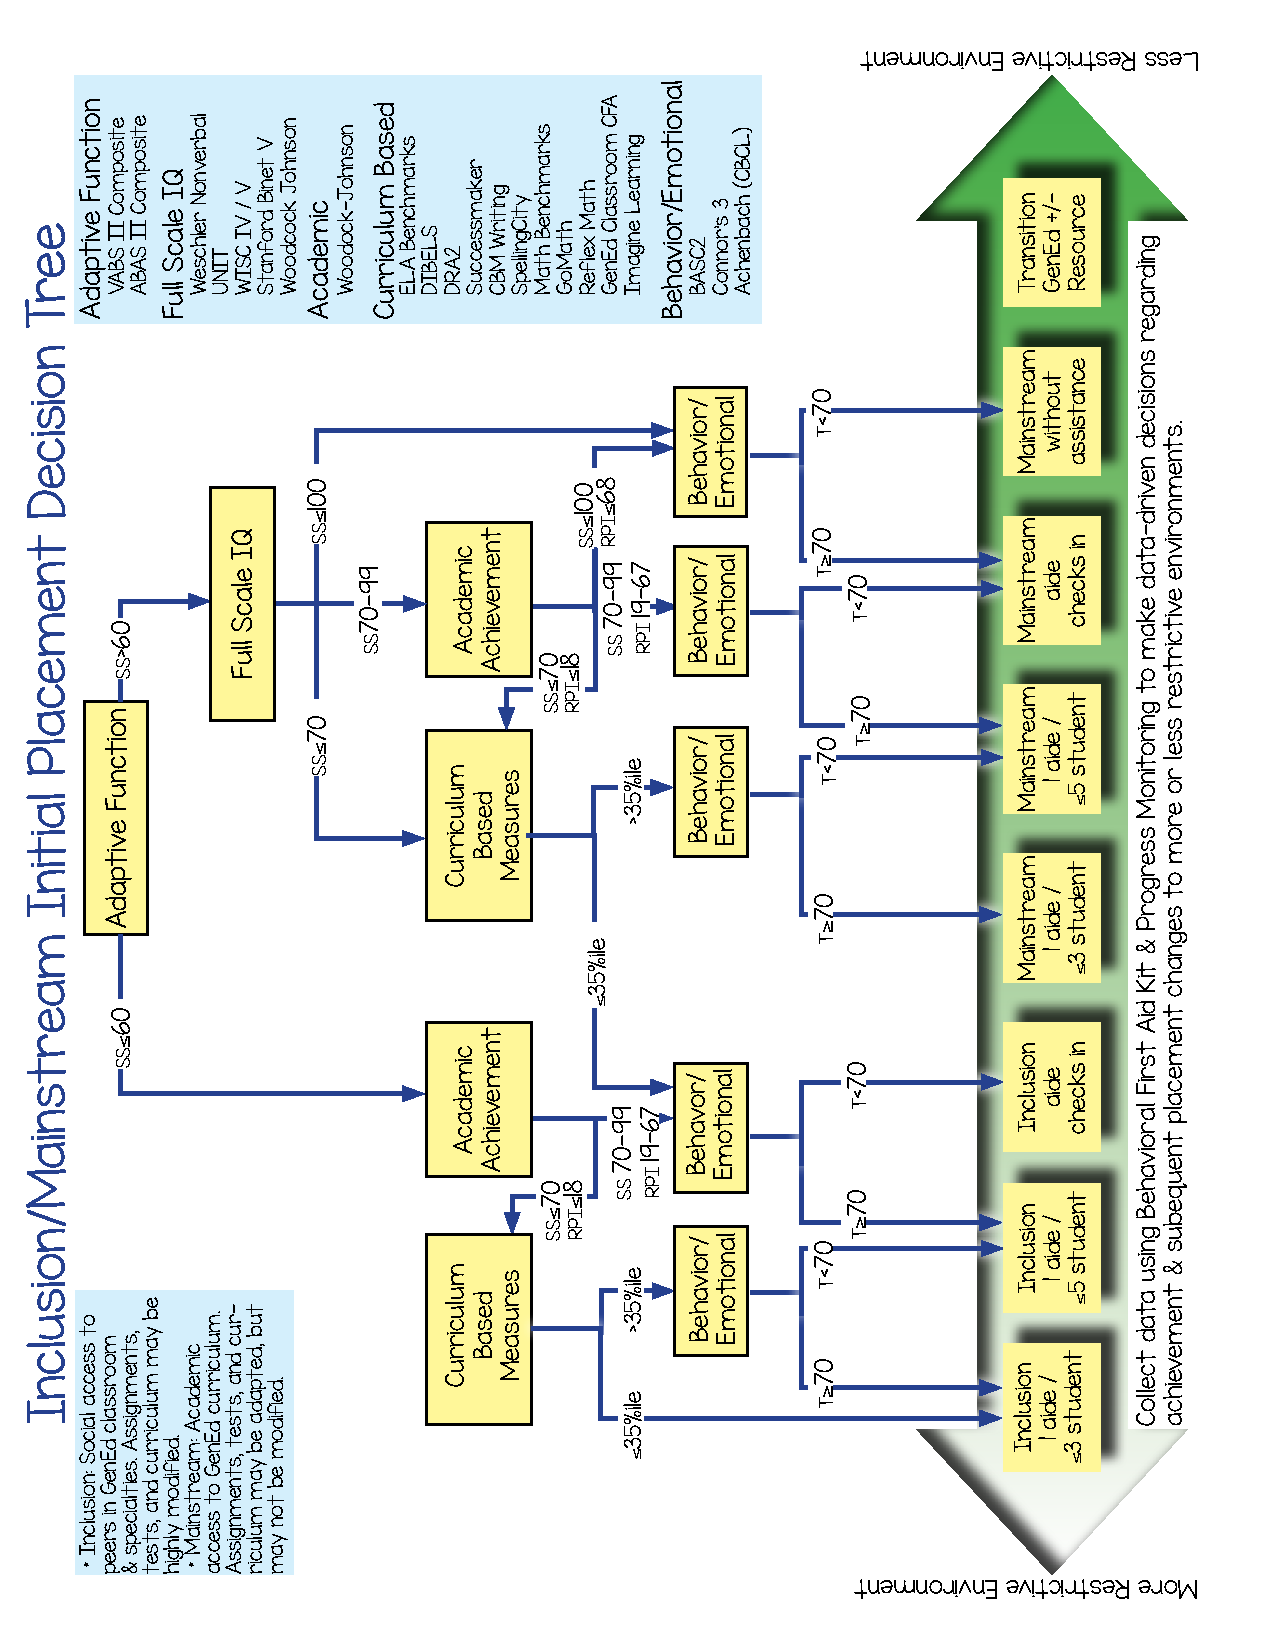
\includepdf[pages={1}]{DecisionTree.pdf}
\chapter{Behavioral Mainstream Decision Tree}
\label{Appendix2}
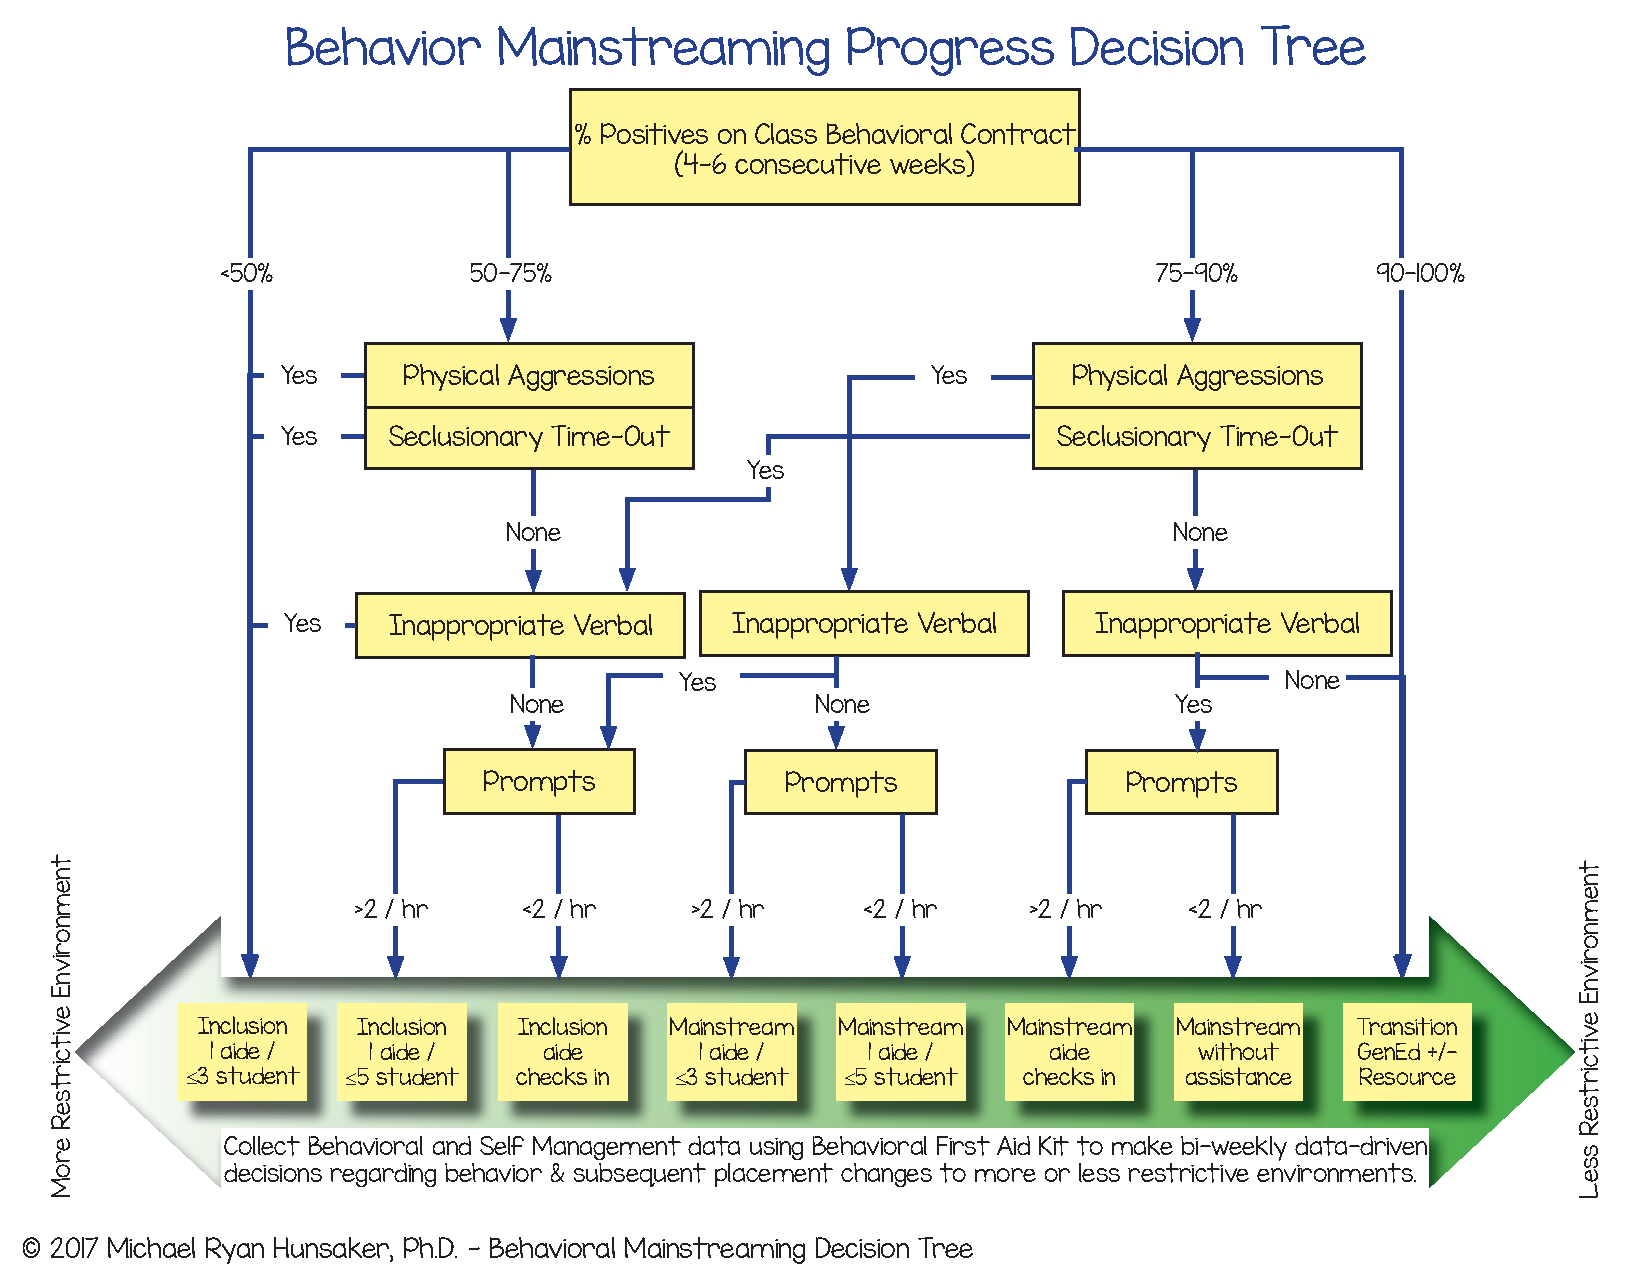
\includepdf[pages={1}]{BehaviorPipeline.pdf}
\chapter{Mainstream Data Sheet} 
\label{Appendix3}
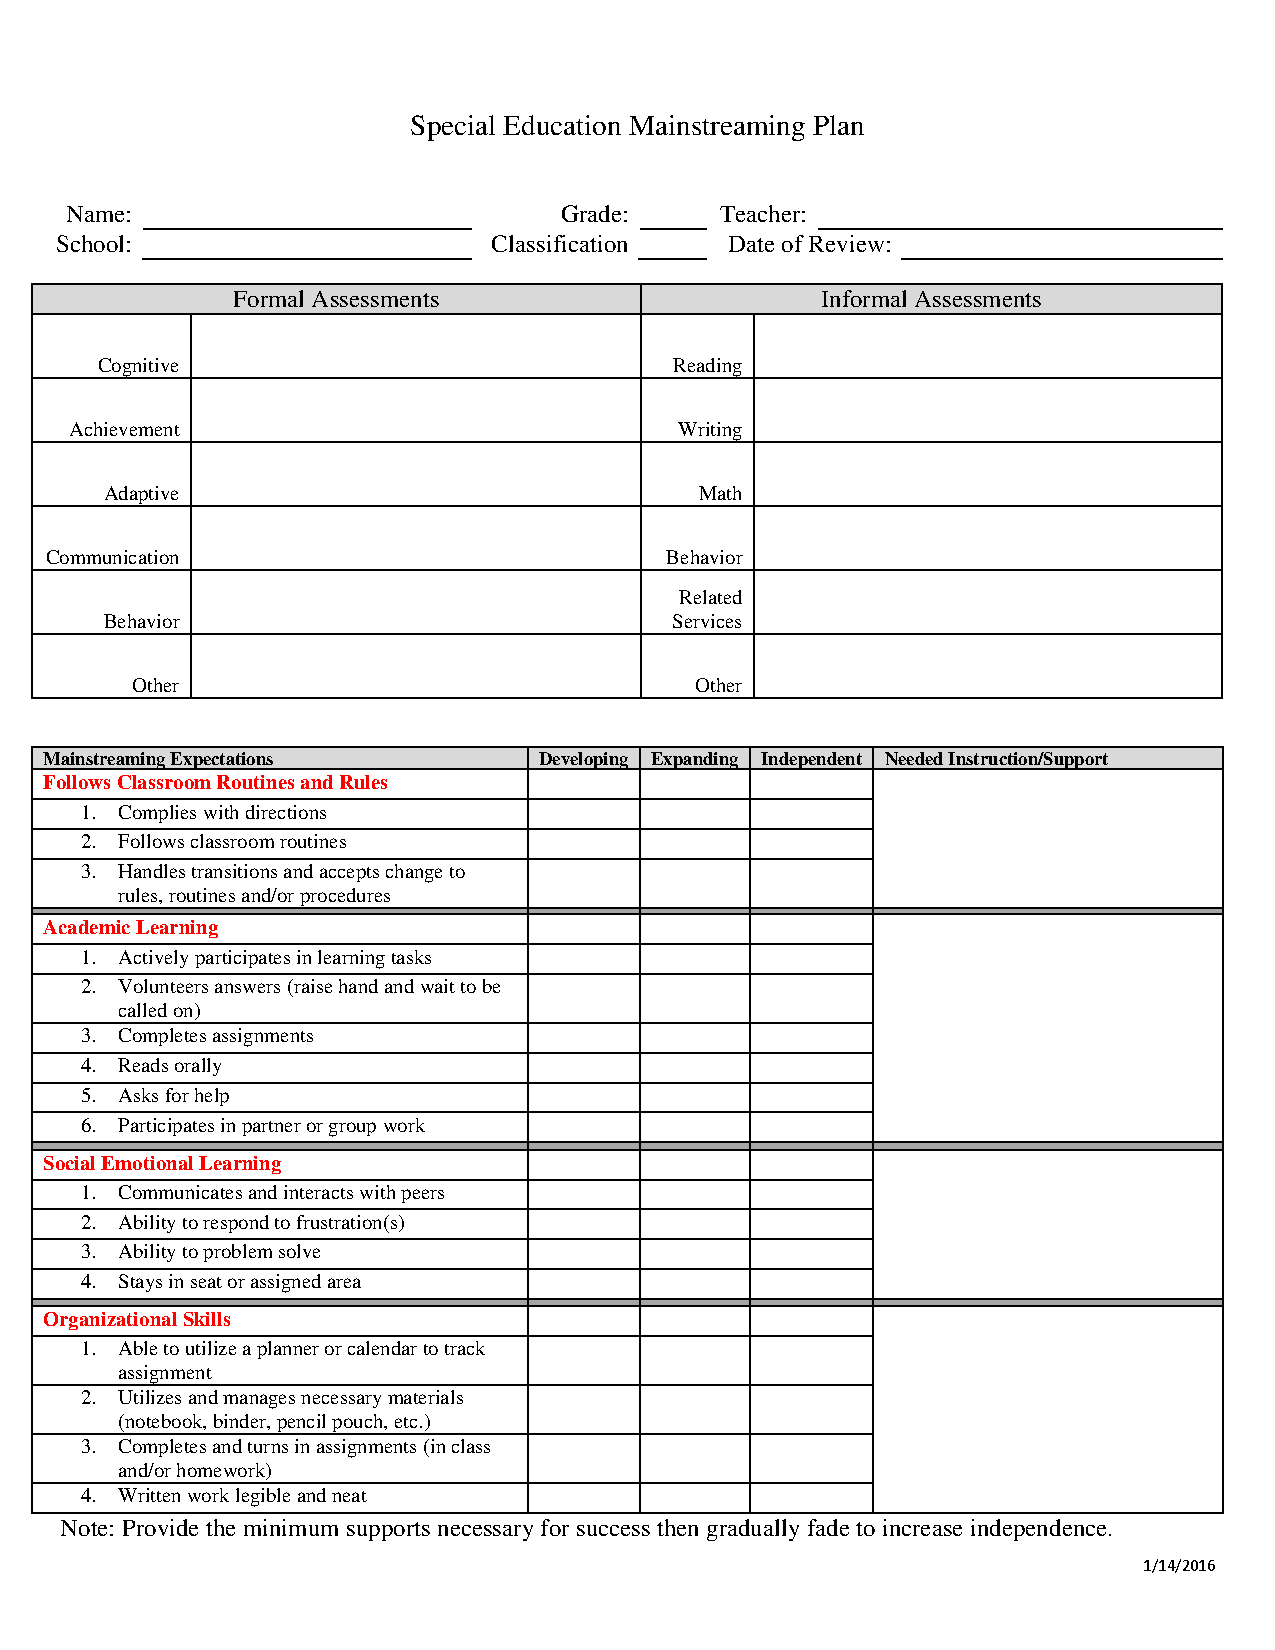
\includepdf[pages={1,2}]{MainstreamingPlan.pdf}
\chapter{Classroom Ecological Inventory (K-6)}
\label{Appendix4}
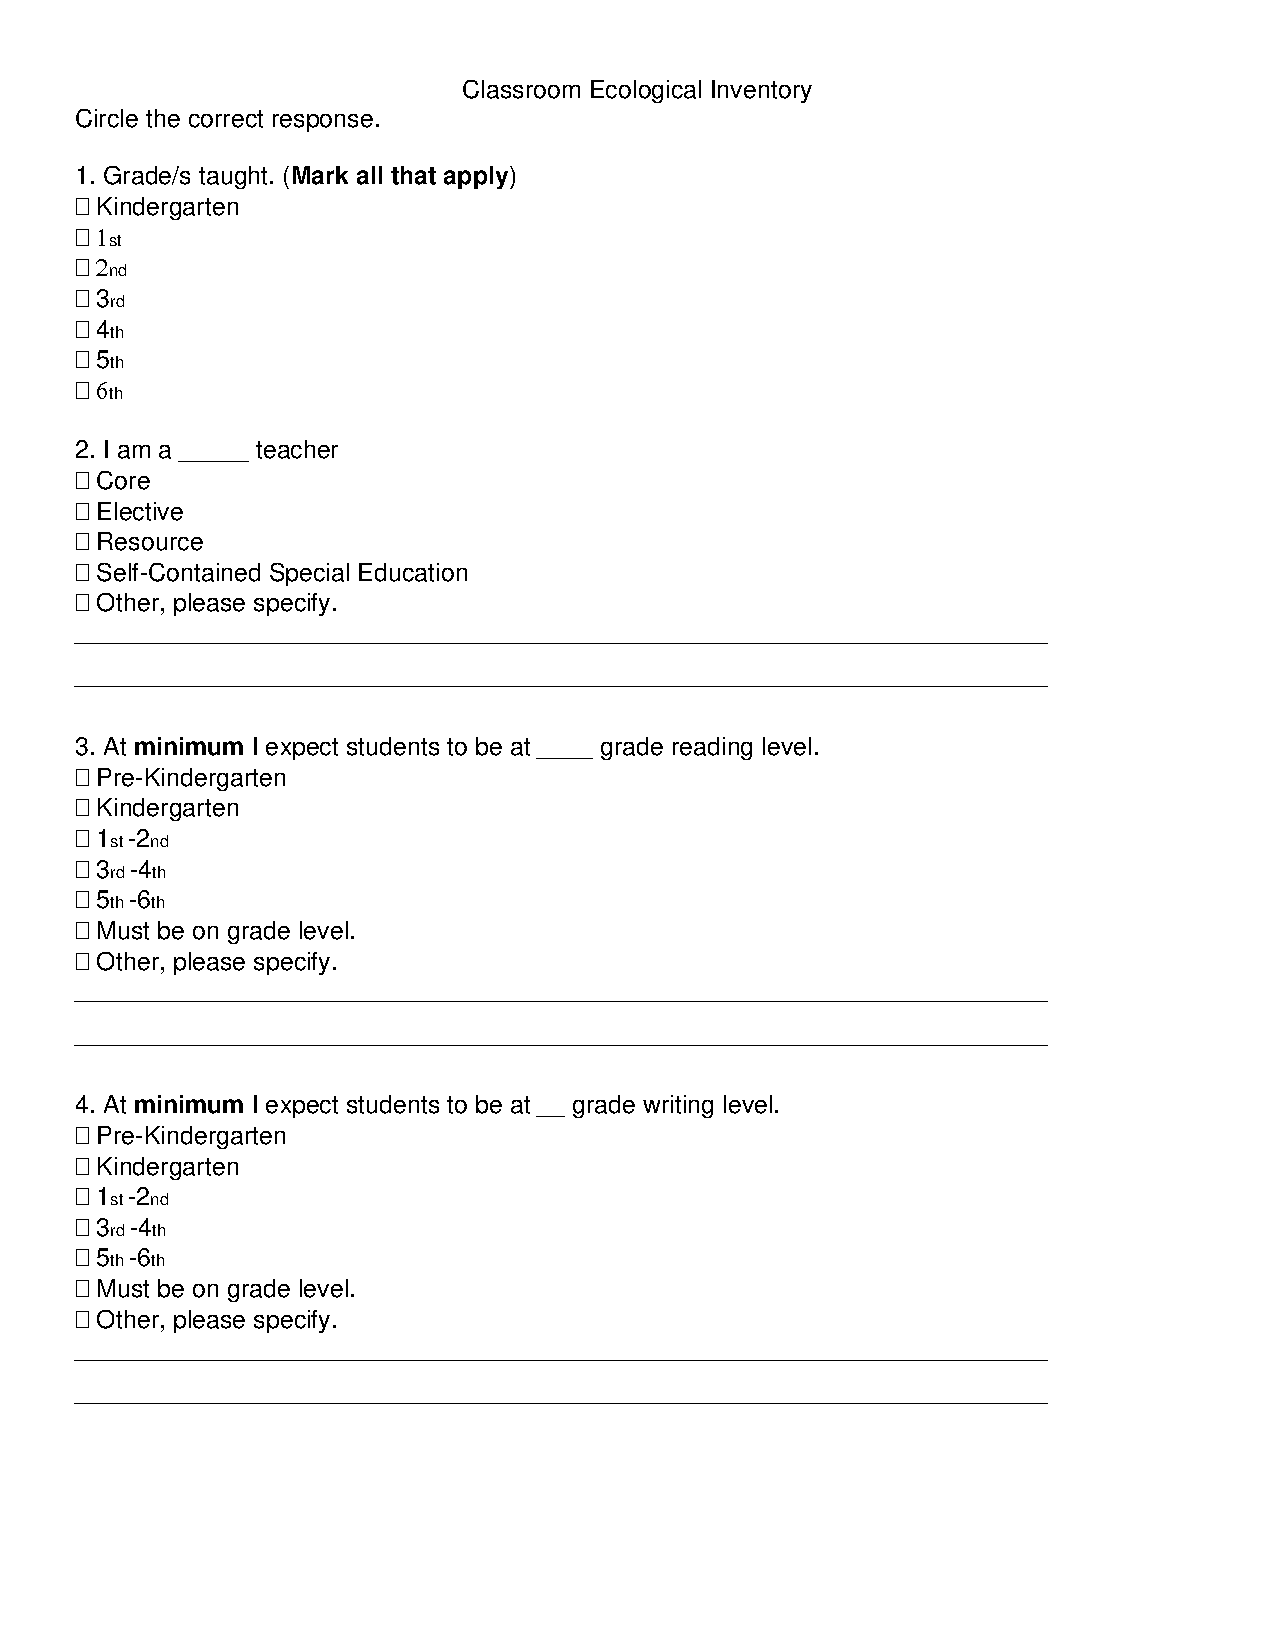
\includepdf[pages={1,2,3,4,5}]{ClassroomEcologicalInventory.pdf}
\chapter{Behavioral First Aid Kit}
\label{Appendix5}
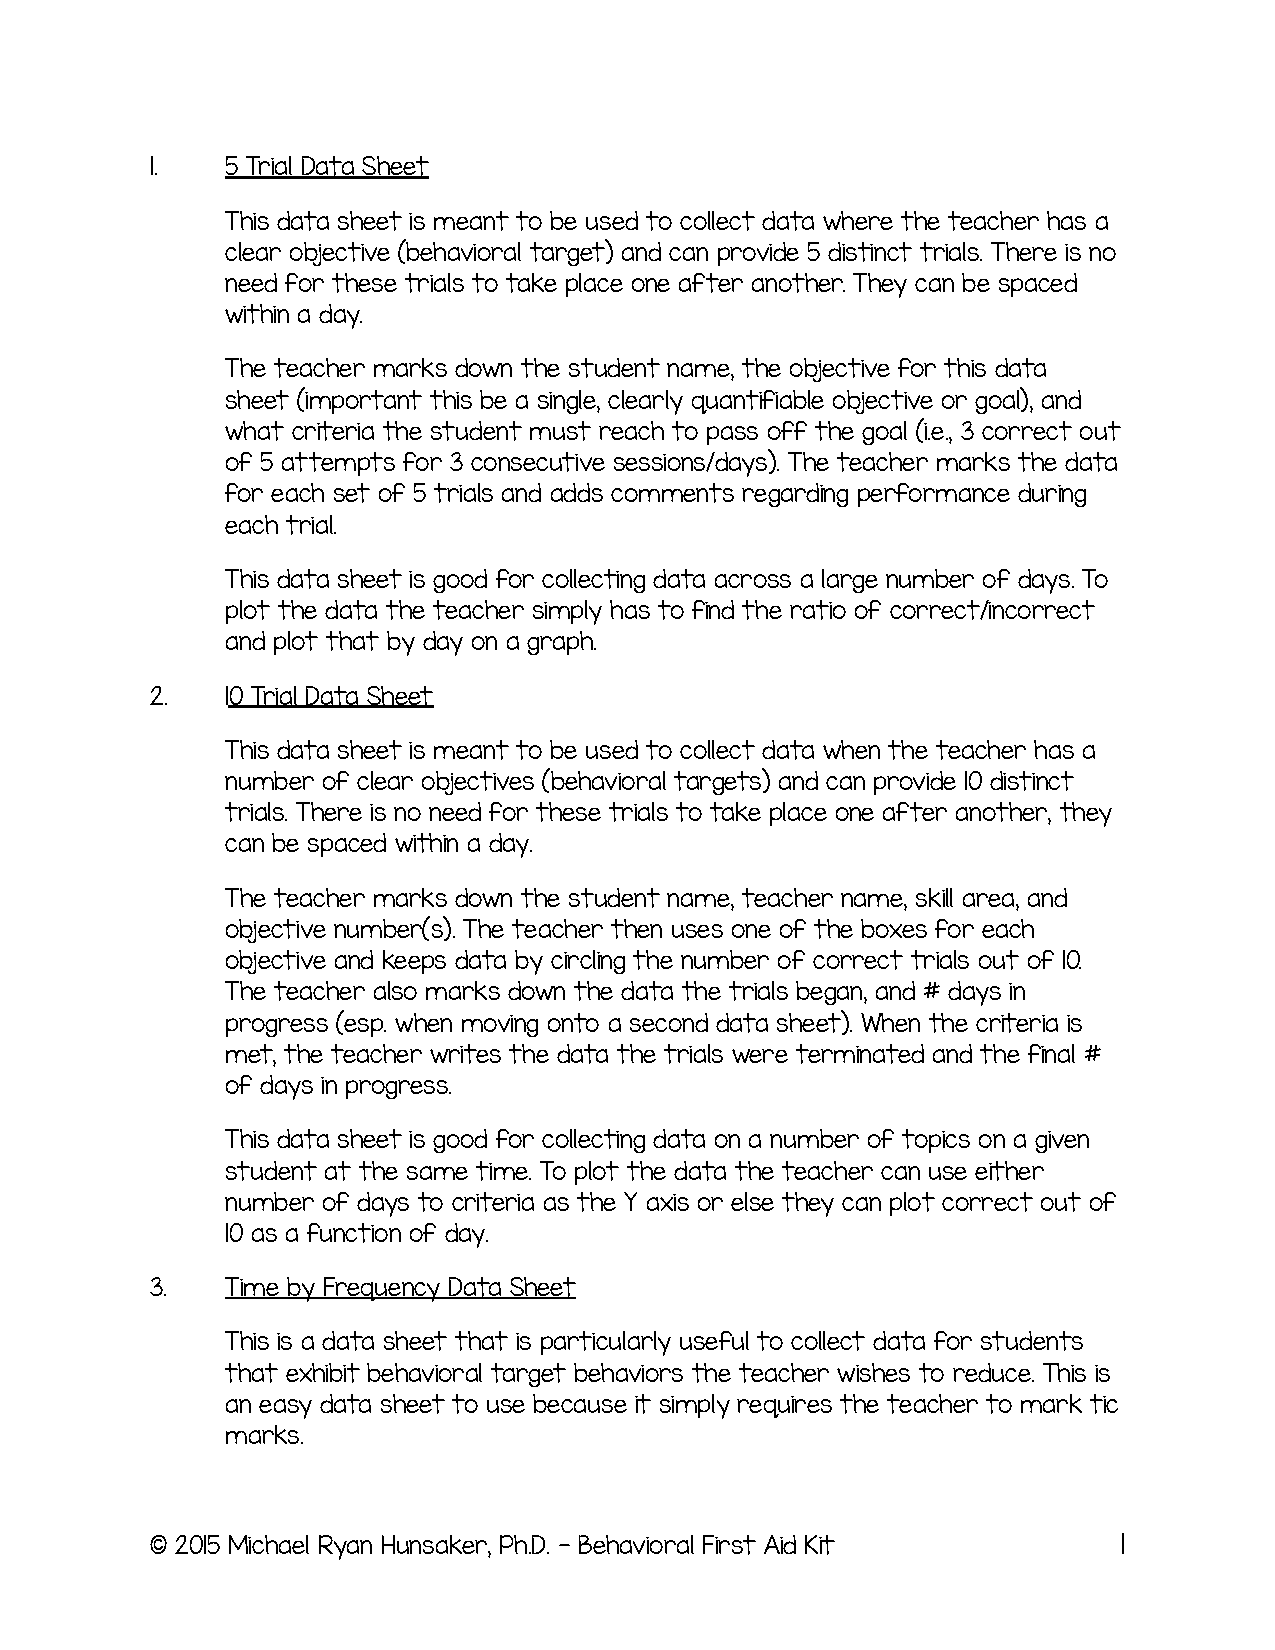
\includepdf[pages={1-56}]{BehavioralFirstAidKit.pdf}
%%%%%%%%%%%%%%%% End Body %%%%%%%%%%%%%%%%%%%%%%%
%
%
%%%%%%%%%%%% Begin Back Matter %%%%%%%%%%%%%%%%%%%
\backmatter
\addcontentsline{toc}{part}{Notes and Bioliography}
\theendnotes
\printbibliography
\end{document}
